\documentclass[11pt,a4paper,leqno]{report}
\usepackage{tikz}
%\usepackage[german]{babel}
\usepackage{amsmath}
\usepackage{amsthm}
\usepackage{amssymb}
\usepackage{float}
\usepackage{amsfonts}
\usepackage{hyperref}
\usepackage{lmodern}
%\usepackage{makeidx}
%\usepackage{graphicx}
%\graphicspath{{pics/}}
\usepackage{svg}
\usepackage{amsmath}
\usepackage{delarray}
\newcommand{\eps}{\varepsilon}
\newcommand{\R}{\mathbb{R}}
\newcommand{\C}{\mathbb{C}}


%%%%%%%%%%% REST %%%%%%%%%%%%%%%%%%%%%%%%%%%%%%%%%%%%

\DeclareMathOperator{\dom}{dom}
\DeclareMathOperator{\ran}{ran}
\newcommand{\re}{\mathrm{Re}}
\newcommand{\im}{\mathrm{Im}}

\newcommand{\ul}{\underline}
\newcommand{\I}{\mathrm{i}}
\newcommand{\E}{\mathrm{e}}

%\makeindex
%\setlength{\parindent}{0em} 


\newtheorem{theorem}{Theorem}[chapter]
\newtheorem{proposition}{Proposition}[chapter]
\newtheorem{lemma}[theorem]{Lemma}
\newtheorem{definition}[theorem]{Definition}
\newtheorem{corollary}[theorem]{Corollary}
\newtheorem{remark}[theorem]{Remark}

\numberwithin{equation}{chapter}



\usepackage{listings}
\lstset{basicstyle=\ttfamily}
\lstset{literate=%
	{\"o}{{\"O}}1
	{\"a}{{\"A}}1
	{\"u}{{\"U}}1
	{\"u}{{\"u}}1
	{\"a}{{\"a}}1
	{\"o}{{\"o}}1
}
\begin{document}


\begin{titlepage}

\vspace*{5cm}
\begin{center}
\rule{\linewidth}{0.5mm} \\[0.4cm]
{ \Huge \bfseries Mathematik, Berechnung} \\[0.2cm]
{ \Huge \bfseries und Basteleien}\\[0.2cm]
\rule{\linewidth}{0.5mm} \\[3.5cm]
\begin{minipage}[t]{0.4\textwidth}
\begin{flushleft} \large
\emph{Author:}\\
Oliver \textsc{Sko\v{c}ek} \\[4cm]
\small

\end{flushleft}

\end{minipage}
\begin{minipage}[t]{0.4\textwidth}

\end{minipage}
 
% Bottom of the page

 
\end{center}
 
\end{titlepage}

%\maketitle


%\renewcommand{\contentsname}{Contents}

\tableofcontents

\markboth{Contents}{Contents}

\vfill


\chapter*{Einf\"uhrung}
Im Sommer 2019 setzte ich mir in den Kopf ein Projekt zu starten, \"uber das ich schon sehr lange nachgedacht hatte. Der urspr\"ungliche Plan, der vielleicht noch umgesetzt wird, aber zur Zeit auf Eis liegt, war es eine Rechenmaschine wie in den 1930ern zu bauen, basierend auf elektromechanischen Bauteilen wie Relais und einem Lochstreifenleseger\"at. Von der Idee diese Relais selbst zu bauen und zwar aus Parkett Holzleisten, Zimmermannsn\"ageln, Aluminiumfolie und lackiertem Kupferdraht gab ich etwa zur selben Zeit auf wie die Idee Relais zu verwenden. Dies geschah zum einen, weil ich frustriert war mit der Unzverl\"assigkeit der Schaltung und mit der hohen Stromst\"arke von etwa 0.7A, die f\"ur eine Schaltung in meinem Design notwendig war, und zum Anderen geschah es weil ich angefangen hatte mich mit Breadboards und integrierten Schaltkreisen zu besch\"aftigen. 


\chapter{Aufbau einer Rechenmaschine}
Was muss eine Rechenmaschine k\"onnen, damit sie im Prinzip alles berechnen kann, auch wenn sie daf\"ur eine sehr lange Zeit ben\"otigt? Diese Frage wurde Mitte des zwanzigsten Jahrhunderts beantwortet. Mehrere Personen entwickelten unterschiedliche Definitionen des Berechenbaren, und im Laufe der Zeit konnte gezeigt werden, dass all 
iese hypotethischen Rechenmaschinen und Programmiersprachen gleichwertig sind. Die Gleichwertigkeit zwischen einer Rechenmaschine \textbf{A} und einer Rechenmaschine \textbf{B} ist gegeben, wenn die\\ Rechenmaschine \textbf{A} die Rechenmaschine \textbf{B} simulieren kann und umgekehrt. Dies gilt unabh\"angig davon ob es sich um eine analoge Rechenmaschine, eine digitale Rechenmaschine, eine Quantenrechenmaschine oder einen Menschen mit Papier und Stift handelt.\\
\\
Eine Rechenmaschine ist ein Apparat, der Listen von Befehlen abarbeitet und dabei drei fundamentale Bestandteile hat:
\paragraph{Register:} Variablen, Platzhalter, Schmierzettel, et cetera. Ein Ding, dass ein Wort speichern kann, wobei dieses Wort von der Maschine gelesen werden kann und auch durch ein bestimmtes Wort ersetzt werden kann.
\paragraph{Grundoperationen:} Eine Liste von grundlegenden Operation, welche die Maschine auf W\"ortern, Paaren von W\"ortern, et cetera ausf\"uhren kann. Die Ausgabe der Operation muss eindeutig sein und ist wiederum entweder ein Wort, ein Paar von W\"ortern, et cetera. Die Eingabe W\"orter liegen hierbei in bestimmten von der Operation abh\"angigen Registern und die Ausgabew\"orter werden wiederum in bestimmten operationsabh\"angigen Registern abgelegt.
\paragraph{Bedingte Verzweigung:} Ein Weg wie der Ausgang einer Operation die Reihenfolge der abzuarbeitenden Befehle ab\"andern kann. Diese Konstrukte haben f\"ur gew\"ohnlich die Form: "Wiederhole bestimmte Teilliste von Befehlen, bis eine Bedingung erreicht ist"
\\
\\
Der zuletzt beschriebene Bestandteil einer Rechenmaschine, die \textbf{Bedingte Verzweigung} wird oft durch einen internen Zustand der Rechenmaschine realisiert, der f\"ur gew\"ohnlich \"uber so genannte Flaggen implementiert wird. Dies sind Register mit nur einem Bit, die eine Aussage \"uber den Ausgang der letzten Operation macht, welche die Rechenmaschine abgearbeitet hat. Diese Register sind die Ausnahme, sie sind nicht direkt in ihrem Wert setzbar, sondern nur indirekt und zus\"atzlich halten sie kein Wort, sondern genau einen Bit, also null falls die Aussage \"uber die letzte Operation nicht zutrifft und Eins falls doch.\\
\\
In den n\"achsten Kapiteln werden wir uns n\"aher mit den Befehlen, die eine Rechenmaschine abarbeitet auseindandersetze. Zuerst soll hier aber noch der Unterschied und die Beziehung einer Rechenmaschine zum Konzept der Programmiersprache gezogen werden. Programmiersprachen sind Regelwerke nach denen  Text geschrieben werden, der durch eine Rechenmaschine interpretiert und als Kette von Befehlen abgearbeitet werden kann.
Typischerweise hat jede Rechenmaschine eine eigene interne Programmiersprache, welche die Maschinenbauteile interpretieren k\"onnen und somit die Berechnung ausf\"uhren die wir uns w\"unschen.\\
\\
Jede Programmiersprache besteht aus elementaren Bausteinen, Gundsymbolen oder W\"ortern, die Variablen, Befehle, Operationen, Zuweisungen oder\\ Verzweigungsanweisungen repr\"asentieren und aus Regeln, die festlegen welche Ketten dieser Grundsymbole Ausdr\"ucke der Programmiersprache sind, also valide oder syntaktisch korrekte Programme. Ein Programm ist nichts anderes als ein Ausdruck, der die sprachlichen Regeln einer Programmiersprache erf\"ullt.\\
\\
Synonym zum Begriff des Programms ist der Begriff des Algorithmus. \\
Programmieren ist das entwerfen von Programmen. Jeder der noch nichts damit zu tun hatte, kann sich das komplett analog zu einem Koch vorstellen, der ein Rezept f\"ur einen unf\"ahigen Lehrling schreibt. Das Rezept ist eine Abfolge an Operationen, die der Lehrling an der K\"uche ausf\"uhren muss, um ein Gericht herzustellen. Der Lehrling ist unf\"ahig und deshalb muss man es ihm ganz genau aufschreiben, also pr\"azise formuliert, nach gewissen Regeln, damit die Anweisung immer eindeutig ist und keine Interpretationsfreiheit zul\"asst. Genauso verh\"alt es sich mit der Programmierung einer Rechenmaschine.
\newpage
\section{GOTO-Programme}
Eine der einfachsten und am leichtesten verst\"andlichen Arten von Programmier- sprachen ist die Klasse der GOTO-Programmiersprachen. In der Praxis sind GOTO-Programmiersprachen zwar nur von geringer Bedeutung, da sich Programme, die in solchen Sprachen geschrieben wurden, wegen ihrer schwierigen Lesbarkeit, nur schwer warten lassen, jedoch sind die internen Maschinensprachen von allen Rechenmaschinen, die in der Praxis eingesetzt werden, GOTO-Programmiersprachen und (theoretisch interessant).\\
\\
Es folgt eine Beschreibung einer sehr einfachen Form einer GOTO-Programmier- sprache, die bereits alle Zutaten f\"ur eine universelle Programmiersprache enth\"alt, und die wir fortan als Ausgangspunkt f\"ur unsere Diskussion des Berechenbaren ansehen.
\paragraph{Variablen:} Variablen sind synonym zu verstehen mit Registern, es sind also Dinge die ein Wort speichern k\"onnen, das gelesen werden kann, und durch ein anderes Wort ersetzt werden kann. Ein Wort wird in der folgenden Diskussion, um m\"oglichst einfach zu bleiben, eine nat\"urliche Zahl sein. \\
\begin{definition}
	Ein GOTO-Programm ist durch folgendes Schema definiert:
	\begin{enumerate}
		\item Das Kopieren des Wertes einer Variablen $X$ auf eine Variable $Y$, kurz $Y = X$, ist ein GOTO-Programm.
		\item Einer Variable $X$, einen bestimmten Wert $A$ geben, kurz $X = A$\footnote{A ist zum Beispiel 12, daher kurz $X = 12$.}, ist ein GOTO-Programm.
		\item Einer Variablen $Z$ die Summe zweier Variable $X$ und $Y$ als Wert zuordnen, kurz $Z = X + Y$, ist ein GOTO-Programm.
		\item Einer Variablen $Z$ die Differenz zweier Variable $X$ und $Y$ als Wert zuordnen, kurz $Z = X - Y$, ist ein GOTO-Programm.\footnote{Da wir mit nat\"urlichen Zahlen und keinen ganzen Zahlen arbeiten, setzen wir eine Differenz, die in einer negativen Zahl resultiren w\"urde auf den Wert Null.}
		\item Das Stoppen des Programmes, kurz $HALT$ ist ein GOTO-Programm.
		\newpage
		\item Seien $W$ und $V$ GOTO-Programme, dann ist
		\begin{lstlisting}
			W
			V
		\end{lstlisting}
		ein GOTO-Programm. Daher zwei GOTO-Programme untereinander- geschrieben bilden ein GOTO-Programm. Praktisch bedeutet dies, dass zuerst das obere Programm und dann das untere Programm ausgef\"uhrt wird. Beispiel:
		\begin{lstlisting}
		X = Y
		Z = X + Y
		\end{lstlisting}
		Hier wird der Variable $X$ der Wert der Variablen $Y$ zugeordnet und anschlie\ss{}end wird der Variablen $Z$ die Summe der Variablen $X$ und $Y$ zugeordnet.
		\item Das Springen zu der $n$-ten Zeile des GOTO-Programms, falls die Variable $X$ einen Wert ungleich Null aufweist, und nichts tun falls es einen Wert gleich null hat, kurz $\text{IF }X\text{ GOTO }n$.\\
		Beispiel (Arithmetische Multiplikation): 
		\begin{lstlisting}
		X = 0
		X = X + Y
		Z = Z - 1
		IF Z GOTO 2
		\end{lstlisting}
	\end{enumerate}
\end{definition}	
Das Beispielprogramm unter Punkt sieben beschreibt die Multiplikation zweier nat\"urlicher Zahlen $Z$ und $Y$, daher wenn das Programm zu Ende gelaufen ist, steht in der Variable $X$ das Produkt der Werte, die zum Start des Programmes in der Variablen $Z$ und $Y$ gespeichert waren. Es ist zu beachten, dass wir eins basiert nummerieren. Also mit Zeilennummerierung als Orientierung sieht unser Programm so aus:
\begin{lstlisting}
	1: X = 0
	2: X = X + Y
	3: Z = Z - 1
	4: IF Z GOTO 2
\end{lstlisting}			
Wie nicht unschwer zu erkennen ist, steckt der Grund warum wir dies eine GOTO-Programmiersprache nennen im siebten Punkt der Definition. Dieser Punkt legt fest wie bedingte Verzweigung in der Programmiersprache funktioniert. Im Laufe der n\"achsten Kapitel werden wir weitere M\"oglichkeiten kennen lernen wie man dies bewerkstelligen kann.
\paragraph{\"Ubungsbeispiel 1:} Schreibe ein GOTO-Programm, dass die Fakult\"at einer nat\"urlichen Zahl $n$ berechnet, kurz $n!$. Die Fakult\"at ist rekursiv definiert durch:
$$0! = 1$$
$$(n + 1)! = (n + 1) * n!$$
In einer einzigen Formel l\"asst sie sich aber auch, weniger pr\"azise, folgenderma\ss{}en definieren:
$$n! = n * (n - 1) * \dots * 2 * 1$$
Beispiel: $5! = 5 * 4 * 3 * 2 * 1$
\subsection{Grundoperationen}
Die Grundoperationen unserer GOTO-Programmiersprache sind die Summe und die Differenz zweier nat\"urlicher Zahlen. Alternativ gibt es aber auch noch andere m\"ogliche Operationen, die in Kombination unsere Grundoperationen ausdr\"ucken k\"onnen und damit genauso Kandidaten f\"ur Grundoperationen sind. Hier wollen wir kurz ein paar Beispiele bringen.
\paragraph{Nachfolger und Vorg\"anger}
Alternativ zur Addition und Subtraktion kann man auch die einstellige Operation des Nachfolgers ($S(n) = n + 1$) und seiner Umkehroperation Vorg\"angers ($T(n) = n - 1$)\footnote{Es soll gelten $T(0)=0$.} einer nat\"urlichen Zahl verwenden. Offensichtlich l\"asst sich die Addition in diesen Operationen ausdr\"ucken:
\begin{lstlisting}
	1: X = S(X)
	2: Y = T(Y)
	3: IF Y GOTO 1
\end{lstlisting}	
\paragraph{\"Ubungsbeispiel 2:} Zeige wie sich die Subtraktion durch $S$ und $T$ in einem GOTO-Programm ausdr\"ucken l\"asst.
\paragraph{Nachfolger und Gleichheit} Die Vorg\"angeroperation l\"asst sich auch durch eine Gleichheitsrelation austauschen. Relationen sind Operationen, die als Resultat entweder Null f\"ur falsch oder Eins f\"ur wahr ausgeben. In unserem Fall nimmt die Operation zwei nat\"urliche Zahlen $X$ und $Y$ und schreibt eine Eins, falls die Werte gleich sind, und sonst eine Null, in die Variable $Z$. \\Als Operation schreiben wir dies als: $Z = (X == Y)$.
\paragraph{\"Ubungsbeispiel 3:} Zeige wie sich die Vorg\"angeroperation durch die\\ Nachfolgeroperation und die Gleichheitsrelation in einem GOTO-Programm ausdr\"ucken l\"asst.
\paragraph{\"Ubungsbeispiel 4:} Zeige wie sich die Gleichheitsrelation in in der urspr\"unglichen Definition eine GOTO-Programms ausdr\"ucken l\"asst.
\section{WHILE-Programme}
Eine, wegen ihrer leichteren Lesbarkeit, beliebtere Klasse von Programmiersprachen sind die WHILE-Programmiersprachen. Die meisten modernen Programmiersprachen sind unter anderem auch WHILE-Programmiersprachen.\\
\\
Es folgt nun wie bei den GOTO-Programmen eine Beschreibung einer einfachen Form einer WHILE-Programmiersprache. Der einzige Untschied zu GOTO-Programmen liegt im siebenten Punkt der Definition, n\"amlich der Implementierung bedingter Verzweigungen.
\begin{definition}
	Ein WHILE-Programm ist durch folgendes Schema definiert (\"ubernehme Punkt 1-6 von der Definition eines GOTO-Programmes, lies einfach wo auch immer GOTO-Programm geschrieben steht, WHILE-Programm):
	\begin{enumerate}
 		\setcounter{enumi}{6}
		\item Wenn $X$ ein WHILE-Programm ist und $Z$ eine Variable, dann ist: 
		\begin{lstlisting}
			WHILE Z:
			    X
		\end{lstlisting}
		auch ein WHILE-Programm. Es bedeutet, dass das WHILE-Programm X solange ausgef\"uhrt wird bis die Variable $Z$ Null ist.\\
		Beispiel:(Arithmetische Multiplikation)
		\begin{lstlisting}
		X = 0
		WHILE Z:
		    X = X + Y
		    Z = Z - 1
		\end{lstlisting}	
		Wir sehen hier, wie bereits f\"ur GOTO-Programme gemacht ein WHILE-Programm, das das Produkt zweier nat\"urlicher Zahlen $X$ und $Z$ berechnet. 
	\end{enumerate}
\end{definition}
An diesem einfachen Beispiel l\"asst sich wenn wir es mit dem zugeh\"origen GOTO-Programm vergleichen bereits erkennen, dass und inwiefern WHILE-Berechenbarkeit und GOTO-Berechenbarkeit equivalent sind, also sich zu jedem GOTO-Programm ein WHILE-Programm finden l\"asst und umgekehrt, dass daselbe berechnet. Was uns sogleich zum n\"achsten Abschnitt f\"uhrt.
\paragraph{\"Ubungsbeispiel 5:} Mach \"Ubungsbeispiel 1, 2 und 3 mit WHILE-Programmen, anstelle von GOTO-Programmen.
\section{Church-Turing Hypothese}
Die Church-Turing Hypothese (CT-Hypothese) ist eine nicht beweisbare Aussage \"uber, dass was im Prinzip berechenbar ist. Inspiriert ist sie durch die Erkenntnis, dass alle Defintionen des Berechenbaren, also im Prinzip \\Programmiersprachen, zumindest die Berechnungen ausf\"uhren kann, die GOTO-Programme berechnen k\"onnen. CT-Hypothese besagt also, dass jede Berechnung die im Prinzip m\"oglich ist von einer Maschine ausgef\"uhrt werden kann, die GOTO-Programme verarbeiten kann. Hiermit ist auch klar weshalb die Aussage eher philosophisch und nicht beweisbar ist, da "das Berechenbare" nicht leicht fassbar/definierbar ist und wir heute nicht wissen k\"onnen was morgen noch f\"ur Maschinen sein werden und welchen Gesetzen sie gehorchen werden. Es sei weiters noch angemerkt, dass wir aus ersichtlichem Grund die GOTO-Programmiersprache, sowie jede Programmier-sprache, die jede Berechnung ausf\"uhren kann, die von einem GOTO-Programm ausgef\"uhrt werden kann, eine universelle Programmiersprache genannt werden soll. Eine solche universelle Programmiersprache ist sozusagen maximal in ihrer F\"ahigkeit Berechnungen auszuf\"uhren. Zur Motivation der Hypothese werden wir als n\"achstes beweisen, dass zu jedem GOTO-Programm ein WHILE-Programm existiert, dass daselbe berechnet und umgekehrt
\paragraph{IF THEN END} Doch bevor wir dies zeigen soll eine bedingte Verzweigung eingef\"uhrt werden, die zwar nicht zwingend notwendig ist, daher wir k\"onnen sie mit WHILE-Programmen sowie GOTO-Programmen bereits ausdr\"ucken, aber sie werden, die in unseren Beweisen vorkommenden Programme kompakter und leichter lesbar machen, wenn wir sie verwenden.
\begin{definition}
Sei $Z$ eine Variable, $P$ und $Q$ sind GOTO/WHILE-Programme, dann nennen wir das Konstrukt
	\begin{lstlisting}
	IF Z THEN
		P
	Q
	\end{lstlisting}
eine IF THEN END Anweisung und sie bedeutet, dass falls $Z$ ungleich Null ist, dann wird $P$ ausgef\"uhrt und anschlie\ss{}end $Q$, andererseits falls $Z$ gleich Null ist, dann \"uberspringen wir $P$ und f\"uhren gleich $Q$ aus.
\end{definition}

\paragraph{\"Ubungsbeispiel 6:} Schreibe ein GOTO-Programm, dass dieselbe Berechnung ausf\"uhrt wie das oben beschriebene IF THEN END Konstrukt.

\paragraph{\"Ubungsbeispiel 7:} Schreibe ein WHILE-Programm, dass dieselbe Berechnung ausf\"uhrt wie das oben beschriebene IF THEN END Konstrukt.

\paragraph{\"Ubungsbeispiel 8:} Schreibe ein WHILE-Programm, dass dieselbe Berechnung ausf\"uhrt wie das oben beschriebene IF THEN END Konstrukt.

\paragraph{\"Ubungsbeispiel 9:} Zeige wie sich die Gleichheitsrelation als WHILE-Programm ausdr\"ucken l\"asst.
\begin{proof}
\textbf{WHILE $\rightarrow$ GOTO:} Gegeben sei ein WHILE-Programm, wir k\"onnen nun jedes Vorkommnis einer WHILE-Struktur
\begin{lstlisting}
		WHILE Z:
			P 
\end{lstlisting}
nach folgendem Schema schrittweise durch eine GOTO-Struktur ersetzen:
\begin{lstlisting}
		n - 2: X = 1 - Z
		n - 1: IF X GOTO m + 1
		n    : P
		m    : IF Z GOTO n
\end{lstlisting}
wobei $n$ die Nummer des ersten Befehls im Programm $P$ ist und die Rollen von $X$ und $Z$ so zu verstehen sind, dass zu jeder Variablen $Z$ eine eigene Variable $X$ erzeugt werden soll, die sonst nirgendwo verwendet wird.\\
Wenn dieser Prozess abgeschlossen ist, haben wir ein zu unserem urspr\"unglichen WHILE-Programm, equivalents GOTO-Programm erzeugt.
\\
\\
\textbf{GOTO $\rightarrow$ WHILE:} Gegeben sein ein GOTO-Programm $P$. Wir starten mit der Konstruktion eines equivalenten WHILE-Programmes $Q$ indem wir die ersten beiden Zeilen schreiben:
\begin{lstlisting}
	Y = 1
	WHILE Y
		X = 0
\end{lstlisting}
Wir r\"ucken nun ein und der Rest des Programmes, dass wir konstruieren wird nun innerhalb dieser initialen WHILE-Anweisung laufen. Falls die Variable $Y$ bereits in $P$ vorkommt, w\"ahle anstelle von $Y$ eine Variable, die nicht in $P$ vorkommt.\\
\\
Anschlie\ss{}end f\"ugen wir f\"ur jede Zeile im Programm $P$, der Reihe nach einen Segment folgender Form am unteren Ende von $Q$, mit der Einr\"uckung der ersten Zeile nach dem ersten WHILE, hinzu.\footnote{Da unsere WHILE-Programmiersprache keine IF THEN END Anweisungen enthalten, stehen die IF THEN END Anweisungen hier f\"ur ein funktionales equivalent in unserer WHILE-Programmiersprache.}
\begin{lstlisting}
	Z = (X == K)
	IF Z THEN
		'Befehl von Programm P in der Zeile K'
		X = X + 1
\end{lstlisting}
Falls der Befehl in der $K$-ten Zeile von $P$ eine Sprunganweisung ist, ersetzen wir den dort stehenden Befehl:\footnote{$R$ steht hier f\"ur die im Befehl vorkommende Variable.}
\begin{lstlisting}
IF R GOTO n
\end{lstlisting}
durch
\begin{lstlisting}
IF R THEN
	X = n
\end{lstlisting}
ansonsten schreiben wir den Befehl so wie er in $P$ steht an die entsprechende Position. Das so erzeugte WHILE-Programm ist equivalent zum urspr\"unglichen GOTO-Programm.
\end{proof}

Abschlie\ss{}end sei noch erw\"ahnt, dass die CT-Hypothese nichts \"uber die Anzahl der Rechenschritte oder die Zeit, die eine Machine zur Berechnung ben\"otigen wird aussagt. Ein Quantencomputer wird eine Faktorisierung einer gro\ss{}en nat\"urlichen Zahl in kurzer Zeit vollbringen, w\"ahrend eine klassischer Computer Jahrhunderte braucht. Aber diesen Aspekt von unterschiedlichen Programmiersprachen und Maschinen haben wir bereits gesehen, als wir untschiedliche Grundoperationen f\"ur GOTO-Programme in betracht gezogen haben.

\section{Kleenesche Normalform}
Im vorangegangenen haben wir gesehen, wie zu jedem GOTO-Programm ein equivalentes WHILE-Programm erzeugt werden kann und umgekehrt.\\
Wir modifizieren nun unsere WHILE-Programmiersprache, indem wir IF THEN END Anweisungen hinzuf\"ugen. Die resultierende Sprache nennen wir WHILE/IF-Programmiersprache. Sie ist equivalent zu unsere WHILE-Programmiersprache, da sich IF THEN END durch WHILE Anweisungen ausdr\"ucken l\"asst, aber erlaubt nun die Konstruktion einer Kleenschen Normal- form zu einem gegebenen WHILE-Programm.\\
\\
Wir folgen nun dem Beweis aus dem letzten Abschnitt.\\
Gegeben ist ein WHILE-Programm $P$, wir wandeln es in ein equivalentes GOTO-Programm $Q$ um, und konstruieren anschlie\ss{}end wie im Beweis ein equivalentes WHILE/IF Programm, dass nur mehr eine einzelne WHILE-Anweisung besitzt. 
\paragraph{Beispiel:} Gegeben sei folgendes WHILE-Programm, welches \"uberpr\"uft ob eine gegebene Zahl eine Primzahl ist.
\paragraph{\"Ubungsbeispiel 10:}
\newpage
\chapter{Zahlensysteme}
Bislang haben wir Programmiersprachen als etwas angesehen, dass Operationen auf nat\"urlichen Zahlen ausf\"uhrt. Bislang haben wir darauf verzichtet genauer darauf einzugehen, was genau eine nat\"urliche Zahl ist und wie sie in einer physischen Rechenmaschine dargestellt werden k\"onnen.
Eine Rechenmaschine wird nie beliebig gro\ss{}e nat\"urliche Zahlen darstellen k\"onnen, da sie immer limitiert sein wird in der Anzahl der wohlunterscheidbaren Zust\"ande die sie annehmen kann.%\\
%\\
%In diesem Kapitel wird eine neue an GOTO-Programmiersprachen angelehnte Programmiersprache verwendet, die im Gegensatz zu unserer urspr\"unglichen Definition nicht auf nat\"urlichen Zahlen operieren, sondern auf Symbolen.\\
%\\
%\textbf{Variablen} speichern wie gehabt ein Wort, aber W\"orter sind von hier an nicht mehr nat\"urliche Zahlen sondern Symbole aus einer vorgegebenen Liste von Symbolen.\\
%\\
%Hier ist der richtige Zeitpunkt um ein wichtiges Konzept der Computerwissenschaften kennen zu lernen, den Stack.
%Ein \textbf{Stappel} oder Stack ist eine Art von Speicher, der sich wie ein Stappel Notizzettel verh\"alt. Er erlaubt zwei Operationen, n\"amlich das Legen einer Notiz oben auf den Stappel oder das Nehmen der obersten Notiz vom Stappel. 
%\begin{definition}
%	Sei $X$ eine Variable; ein Stappel oder Stack $Y$ ist ein Konstrukt bestehend aus einer geordneten Liste von Variablen $Y = \{x_1, x_2, \dots, x_n\}$ mit zwei Operationen.
%	\begin{enumerate}
%	\item\textbf{PUSH $X$ ONTO $Y$}: Sei $\{x_1, x_2, \dots, x_n\}$ der derzeitige Zustand von $Y$, dann wird eine neue Variable $x_{n+1}$ erzeugt, dieser der Wert von $X$ \"ubergeben und anschlie\ss{}end an $Y$ drangeh\"angt. Der neue Zustand des Stacks ist somit: $\{x_1, x_2, \dots, x_n, x_{n+1}\}$
%	\item\textbf{POP $Y$ ONTO $X$}: Sei $\{x_1, x_2, \dots, x_{k-1}, x_k\}$ der derzeitige Zustand von $Y$. Falls $Y$ nicht leer ist, wird die Variable $x_k$ vom Stack genommen, ihr Wert in die Variable $X$ geschrieben und anschlie\ss{}end $x_k$ verworfen. Der neue Zustand des Stacks ist somit: $\{x_1, x_2, \dots, x_{k-1}\}$. Ansonsten wenn $Y$ leer ist, also keine Variable mehr enth\"alt, passiert nichts.
%	\end{enumerate}
%\end{definition}
%Wir kommen nun zur Definition unserer Stack-GOTO-Programmiersprache.
%\begin{definition}
%	Ein Stappel-GOTO-Programm ist durch folgendes Schema definiert:
%	\begin{enumerate}
%		\item Das Kopieren des Wertes einer Variablen $X$ auf eine Variable $Y$, kurz $Y = X$, ist ein GOTO-Programm.
%		\item Einer Variable $X$, einen bestimmten Wert $A$ geben, kurz $X = A$
%		\item Beliebige Stappel/Stack Anweisungen aus Definition 1.4.
%		\item Das Stoppen des Programmes, kurz $HALT$ ist ein GOTO-Programm.
%		\item Seien $W$ und $V$ GOTO-Programme, dann ist
%		\begin{lstlisting}
%		W
%		V
%		\end{lstlisting}
%		ein GOTO-Programm. Daher zwei GOTO-Programme untereinander- geschrieben bilden ein GOTO-Programm. Praktisch bedeutet dies, dass zuerst das obere Programm und dann das untere Programm ausgef\"uhrt wird. Beispiel:
%		\item Das Springen zu der $n$-ten Zeile des GOTO-Programms, falls die Variable $X$ ein vorgegebenes Symbol $S$ tr\"agt, und nichts tun falls dem nicht so ist, kurz $\text{IF }X == S\text{ GOTO }n$.\\
%	\end{enumerate}
%\end{definition}
%Wir haben also wie zu erwarten war, da wir ja keine nat\"urlichen Zahlen mehr haben sondern nur Symbole, die Subtraktion und die Addition gestrichen. Weiters haben wir die Sprunganweisung etwas modifizieren m\"ussen und Stappel/Stack Anweisungen hinzugef\"ugt. Es wird sich in diesem Kapitel zeigen, dass wir von den m\"oglichen Berechnungen, die wir ausf\"uhren k\"onnen nichts verloren haben, jedoch ist diese Stack-GOTO-Programmiersprache in der Praxis relativ unpraktisch, da es sich im Prinzip um eine 1-bit Rechenmaschine handelt.
\\
\\
Bisher sind wir nicht n\"aher auf das Konzept der nat\"urlichen Zahl eingegangen, sondern haben eine gewisses Verst\"andnis desser vorausgesetzt. Hier wollen wir damit brechen und unsere Vorstellungen etwas konkretisieren.
Fangen wir bei Null an, oder eigentlich bei Eins. Was sind die nat\"urlichen Zahlen? Nat\"urliche Zahlen werden verwendet zum Z\"ahlen. Schauen wir uns den Prozess des Z\"ahlens an. 
\section{Der Z\"ahlvorgang} Wir haben zwei Haufen wohlunterscheidbarer Objekte. Einen Haufen Birnen und einen Haufen \"apfel. Wenn wir wissen wollen ob genauso viele Birnen auf dem Birnenhaufen wie \"apfel auf dem \"apfelhaufen sind, k\"onnen wir folgenderma\ss{}en vorgehen. Wir entfernen eine Birne vom Birnenhaufen und einen Apfel vom Apfelhaufen und tun dies so lange bis einer der Haufen verschwunden ist. Wenn beide gleichzeitig verschwinden, dann sind es gleich viele Birnen wie \"apfel, ansonsten gibt es mehr Birnen respektive \"apfel wenn der \"apfelhaufen beziehungsweise der Birnenhaufen zuerst \\verschwunden ist. Durch diesen Prozess ist man in der Lage Anzahlen von allen m\"oglichen Gegenst\"anden durch Haufen von \"apfeln darzustellen. Haufen von \"apfeln sind eine m\"ogliche Darstellung von nat\"urlichen Zahlen. Ein beliebiger Apfelhaufen kann gebildet werden indem man mit einem Apfel startet und schrittweise weitere \"apfel hinzuf\"ugt. Wir w\"unschen uns jetzt aber eine weniger verderbliche und kompaktere Darstellung von nat\"urlichen Zahlen. Hierzu abstrahieren wir unsere \"apfelhaufen. 
\begin{definition} Jede Konstruktion mit den hier beschriebenen vier Eigenschaften nennen wir eine Darstellung der nat\"urlichen Zahlen.
	\begin{enumerate}
		\item Es gibt eine erste nat\"urliche Zahl, wir nennen sie Eins.
		\item Es gibt zu jeder nat\"urlichen Zahl $n$, eine eindeutige n\"achste nat\"urliche Zahl, den Nachfolger $S(n)$.
		\item Alle nat\"urlichen Zahlen werden durch mehrmaliges Nachfolger bilden aus der Eins konstruiert.
		\item Der Nachfolger $S(n)$ einer nat\"urlichen Zahl $n$ unterscheidet sich von $n$ und jeder nat\"urlichen Zahl, die im Bildungsprozess von $n$, also startend bei $1$, \"uber alle Nachfolgerbildungen bis hin zu $n$, auftaucht.
	\end{enumerate}
\end{definition}
%\begin{enumerate}
%	\item Es gibt eine erste nat\"urliche Zahl, wir nennen sie Eins.
%	\item Es gibt zu jeder nat\"urlichen Zahl $n$, eine eindeutige n\"achste nat\"urliche Zahl $S(n)$, die
%	\item Wenn zwei nat\"urliche Zahlen $n$ und $m$ den gleichen Nachfolger haben, also $S(n) = S(m)$, dann sind bereits die beiden gleich, also $n = m$.
%	\item Die Eins ist Nachfolger keiner nat\"urlichen Zahl, also f\"ur jede nat\"urliche Zahl $n$ gilt $S(n)\neq 1$.
%	\item Alle nat\"urlichen Zahlen werden durch mehrmaliges Nachfolger bilder aus der Eins konstruiert
%\end{enumerate}
\begin{proposition}
	Beliebige zwei Darstellungen nat\"urlicher Zahlen sind\\ equivalent\footnote{Equivalent bedeutet hier, dass es eine eindeutig umkehrbare Abbildung gibt, die mit den Nachfolgeroperationen der beiden Darstellungen vertr\"aglich ist.}.
\end{proposition}
\begin{proof}
	Gegeben sind zwei Darstellungen nat\"urlicher Zahlen $A$ und $B$. Wir assozieren nun die Eins von $A$ , kurz $1_A$, mit der Eins von $B$, kurz $1_B$. Falls ein Element $x$ von $A$ mit einem Element $y$ von $B$ assoziert wird dann wird auch der Nachfolger von $x$ bez\"uglich $A$ mit dem Nachfolger von $y$ bez\"uglich $B$ assoziert. 
	Nach Eigenschaft vier aus der Definition der Darstellung nat\"urlicher Zahlen werden unterschiedlichen Elementen von $A$ mit unterschiedliche Elemente von $B$ assoziiert.
	Zusammen mit Eigenschaft drei folgt damit sofort, dass diese Assoziation $\phi$ eine umkehrbar eindeutige Abbildung ist, welche die Nachfolgerabbildung erh\"alt. In Formeln k\"onnen wir den Sachverhalt ausdr\"ucken als:
	$$\phi(S_A(x)) = S_B(\phi(x))$$ f\"ur beliebiges $x$ in $B$, wobei $\phi$ die oben definierte Assoziation ist und $S_A$ beziehungsweise $S_B$ die Nachfolgeroperationen von $A$ respektive $B$ sind.
\end{proof}
\section{Das dekadische Zahlensystem}
In der Schule haben wir eine besonders effiziente Darstellung nat\"urlicher Zahlen kennen gelernt, das dekadische Zahlensystem. Zeigen wir nun, dass diese tats\"achlich nat\"urliche Zahlen im oben beschriebenen Sinn sind.\\
\\
Wir starten mit zehn Symbolen $\{0, 1, 2, 3, 4, 5, 6, 7, 8, 9\}$ und der Einfachheit halber starten wir nicht bei Eins, sondern bei Null. \footnote{Der Startpunkt ist irrelevant, solange es ein erstes Element gibt. Falls notwendig kann man einfach das erste Element nachtr\"aglich entfernen und man hat eine Struktur die bez\"uglich der urspr\"unglichen Struktur mit dem zweiten startet, aber die equivalent zur urspr\"unglichen Struktur ist.}
 
\begin{definition}
	Das dekadische Zahlensystem ist durch folgende Regeln definiert:
	\begin{enumerate}
		\item Die zehn Symbole haben eine feste Reihenfolge $0, 1, 2, 3, 4, 5, 6, 7, 8, 9$. Diese Reihenfolge definiert eine Operation $u$, die ein Symbol nimmt und das n\"achste Symbol in der Reihenfolge ausgibt. Wenn es das Symbol $9$ bekommt gibt es $0$ aus.\\ Daher $u(0)=1$, $u(1)=2$, $u(2)=3$, $u(3)=4$, $u(4)=5$, $u(5)=6$, $u(6)=7$, $u(7)=8$, $u(8)=9$, $u(9)=0$.
		\item Eine dekadische Zahl ist eine endliche Abfolge dieser zehn Symbole. Hierbei schreiben/lesen wir von rechts nach links. Das erste Symbol oder wir sagen die erste Stelle ist das rechteste Symbol. \\Beispiele:
		\begin{lstlisting}
			28420
			  455
			  390
			   89
		\end{lstlisting}
		\item Die Eins des dekadischen Zahlensystems ist:
		\begin{lstlisting}
			1
		\end{lstlisting}
		\item Wir definieren nun die Nachfolgeroperation des dekadischen Zahlensystems als ein Pseudo-GOTO-Programm. \\
		%Sei $y=y_n, \dots, y_2, y_1$ eine dekadische Zahl. Bevor wir das Programm anstarten, befinden sich die Symbole der Stellen von $y$ der Reihe nach im Stack $Y = \{y_n, \dots, y_2, y_1\}$. Weiters gibt es einen Stack $R = \{\}$, der zu Beginn noch leer ist.
\begin{lstlisting}
	1: 'Starte bei der ersten Stelle.'
	2: X = 'Symbol an der derzeitigen Stelle.'
	3: X = u(X)
	4: 'Setze den Wert der derzeitigen Stelle auf X.'
	5: Z = X==0
	6: if Z THEN
	7: 	'Gehe zur n\"achsten Stelle, 
		falls keine Stelle mehr \"ubrig ist 
		f\"uge eine Stelle mit dem Wert 0 hinzu
		und gehe zu dieser Stelle.'
	8:	if Z GOTO 2
	9: HALT
\end{lstlisting}
	\end{enumerate}
\end{definition}
\paragraph{\"Ubungsbeispiel 11:} Spiele den Algorithmus f\"ur einige Beispiele von Zahlen durch um dich mit der Nachfolgeroperation vertraut zu machen.

\begin{corollary}
	Die Stellen des dekadischen Zahlensystems sind selbst ein Zahlensystem.
\end{corollary}
\paragraph{\"Ubungsbeispiel 12:} Beweise Corollary 1.6.
\section{Das bin\"are Zahlensystem}
Nachdem wir uns jetzt das dekadische Zahlensystem angeschaut haben, kommen wir nun zum eigentlichen Thema, dem dualen Zahlensystem oder bin\"aren Zahlen. Im bin\"aren Zahlensystem gibt es im Gegensatz zu den zehn Symbolen des dekadischen Zahlensystem nur zwei Symbole n\"amlich ${0, 1}$. Wie bei den dekadischen Zahlen legen wir eine Reihenfolge der Symbole fest, n\"amlich $0, 1$ und definieren das duale Zahlensystem analog zum dekadischen.\\
%Die Definition des bin\"aren Zahlensystems ist nun ganz einfach. Man nehme die Definition der dekadischen Zahlen und ersetze $\{0, 1, 2, 3, 4, 5, 6, 7, 8, 9\}$ durch $\{0, 1\}$. 
Zur Wiederholung: 
\begin{definition}
	Das dual/bin\"are Zahlensystem ist durch folgende Regeln definiert:
	\begin{enumerate}
		\item Die zwei Symbole haben eine feste Reihenfolge $0, 1$.
		\item Eine bin\"ar Zahl ist eine endliche Abfolge dieser zwei Symbole. Hierbei schreiben/lesen wir von rechts nach links. Das erste Symbol oder wir sagen die erste Stelle ist das rechteste Symbol. \\Beispiele:
		\begin{lstlisting}
		101010
		   101
		   111
		    10
		\end{lstlisting}
		\item Die Eins des dualen Zahlensystems ist:
		\begin{lstlisting}
		1
		\end{lstlisting}
		\item Wir definieren nun die Nachfolgeroperation des dualen Zahlensystems als eine Art GOTO-Programm:
			\begin{lstlisting}
	1: 'Starte bei der ersten Stelle.'
	2: X = 'Symbol an der derzeitigen Stelle.'
	3: X = u(X)
	4: 'Setze den Wert der derzeitigen Stelle auf X.'
	5: Z = X==0
	6: if Z THEN
	7: 	'Gehe zur n\"achsten Stelle, 
		falls keine Stelle mehr \"ubrig ist 
		f\"uge eine Stelle mit dem Wert 0 hinzu
		und gehe zu dieser Stelle.'
	8:	if Z GOTO 2
	9: HALT
			\end{lstlisting}
	\end{enumerate}
\end{definition}
Beispiel: Alle vier stelligen bin\"aren Zahlen
\begin{center}
	\begin{tabular}{c c c c}
		0 & 0 & 0 & 0\\
		0 & 0 & 0 & 1\\
		0 & 0 & 1 & 0\\
		0 & 0 & 1 & 1\\
		0 & 1 & 0 & 0\\
		0 & 1 & 0 & 1\\
		0 & 1 & 1 & 0\\
		0 & 1 & 1 & 1\\
		1 & 0 & 0 & 0\\
		1 & 0 & 0 & 1\\
		1 & 0 & 1 & 0\\
		1 & 0 & 1 & 1\\
	\end{tabular} 

	\begin{tabular}{c c c c}
		1 & 1 & 0 & 0\\
		1 & 1 & 0 & 1\\
		1 & 1 & 1 & 0\\
		1 & 1 & 1 & 1\\
	\end{tabular}  
\end{center}
\paragraph{\"Ubungsbeispiel 13:} Spiele den Algorithmus f\"ur einige Beispiele von Zahlen durch um dich mit der Nachfolgeroperation vertraut zu machen.
\paragraph{\"Ubungsbeispiel 14:} Berechne die bin\"are Darstellung der dekadischen Zahlen $23$, $12$ und $1000$. Finde eine schnelle Methode ohne alle Zahlen von $1$ bis zu der gewissen Zahl durchzugehen.\\
\\
Im Allgemeinen nennen wir Zahlensysteme wie das dekadische oder das duale Zahlensystem Stellenwertsysteme. Im Prinzip m\"ussen wir nur ein paar wohlunterscheidbare Symbole aussuchen, eine Reihenfolge festlegen und wir k\"onnen beliebige derartige Systeme festlegen. In der Informatik ist ein beliebtes Zahlensystem das Hexadezimalsystem. Hier haben wir die Symbole $0, 1, 2, 3, 4, 5, 6, 7, 8, 9, A, B, C, D, E, F$.
\paragraph{\"Ubungsbeispiel 15:} Berechne die hexadezimale Darstellung der dekadischen Zahlen $15$, $17$ und $432$.\\
\\
In der Praxis hat sich das bin\"are Zahlensystem bew\"ahrt, da zum einen eine enge Beziehung zwischen logischen Ausdr\"ucken und dem Zahlensystem und zum anderen unsere Rechenmaschinen elektronisch sind und es praktisch einfacher ist einen Schaltkreis zu bauen, der zwei Zust\"ande kennt, n\"amlich viel Spannung oder Stromst\"arke und sehr wenig Spannung oder Stromst\"arke und es genauso einfacher ist diese zwei Zust\"ande f\"ur einen oder mehrere weiteren Schaltkreis zu unterscheiden. Es gab zwar einige Versuche von Rechenmaschinen mit nicht bin\"arem Zahlen- system, und sogar analoge Rechenmaschinen, die direkt mit reelen Zahlen arbeiten, aber nichts davon konnte die Robustheit der bin\"aren Darstellung und die daraus resultierenden Vorteile schlagen.
%\\

%In einem sp\"ateren Kapitel werden wir einige Elektronik Grundlagen vorstellen und 

%einerseits m\"ussen wir einen Weg finden nat\"urliche Zahlen auf einer Rechenmaschine zuverl\"assig darzustellen und andererseit ein einheitliches Zahlenformat verwenden wollen. Dieses %eiheitliche Zahlenformat ist das Maschinenwort der Rechenmaschine und die Darstellung, die bei elektronischen Rechenmaschinen am sinnvollsten ist, ist die bin\"are Darstellung.
\newpage
\chapter{Aussagenlogik}
Es ist nun an der Zeit, dass wir ein wenig Logik ins Spiel bringen. Logik ist die Lehre vom exakten Schlie\ss{}en; in einfacheren Worten besch\"aftigt sich die Logik damit wie man aus wahren S\"atzen, wiederum wahre S\"atze erzeugt. In diesem Kapitel werden wir uns mit Aussagenlogik oder Boolscher Logik befassen, doch bevor wir in die Tiefen der Logik starten, m\"ussen wir zuerst ein paar Grundbegriffe definieren.\\
\\
Eine \textbf{Aussage} ist ein sprachliches Konstrukt, dass entweder wahr oder falsch ist. Es muss hierbei prinzipiell m\"oglich sein zu \"uberpr\"ufen ob die Aussage zutrifft, also wahr ist oder nicht. Nehmen wir die Aussage:
$$\text{Die vierte Nachkommastelle von }\pi\text{ ist $5$.}$$
Um zu \"uberpr\"ufen ob diese Aussage wahr ist, m\"ussen wir die vierte Nachkomma- stelle der Kreiszahl $\pi$ berechnen und \"uberpr\"ufen ob der resultierende Wert gleich $5$ ist. Was prinzipiell geht und praktisch m\"oglich oder sinnvoll ist, ist oft verschieden, doch ist eine Diskussion dieses Themas hier fehl am Platz.\\
\\ 
Man dr\"uckt den Sachverhalt, dass eine Aussage $\phi$ wahr ist beziehungsweise falsch ist durch den \textbf{Wahrheitswert} von $\phi$ (kurz $w(\phi)$) aus. Wir schreiben den Wahrheitswert $1$, falls die Aussage wahr ist oder $0$, falls die Aussage falsch ist. Pr\"azise formulier hei\ss{}t dies f\"ur den Wahrheitswert einer Aussage $\phi$ schreiben wir:
$$w(\phi)=
\begin{cases} 
	1 & \text{falls $\phi$ wahr ist.} \\
	0 & \text{falls $\phi$ falsch ist.} 
\end{cases}
$$
\textbf{Logische Verkn\"upfung} sind Operationen die eine bestimmte Anzahl von Aussagen nehmen und daraus eine neue Aussage produzieren, deren Wahrheitswert allein von den Wahrheitswerten der Aussagen aus denen sie produziert wurde abh\"angt.\\
\\
Ein Beispiel f\"ur eine jedem bekannte logische Verkn\"upfung, die nur eine einzelne Aussage nimmt und daraus eine neue Aussage produziert, ist die \textbf{Negation} oder Verneinung (kurz $\neg$) einer Aussage. 
$$\neg(\text{Der Himmel ist blau}) = \text{Der Himmel ist nicht blau.}$$
Hierbei gilt, dass die Verneinung die Wahrheitswerte umdreht, daher aus wahr mach falsch und aus falsch mach wahr.
\begin{equation}
w(\neg\phi)= 1 - w(\phi)=
\begin{cases} 
1 & \text{falls }w(\phi)=0\\
0 & \text{falls }w(\phi)=1
\end{cases}
\end{equation}
Das logische \textbf{Und} ist eine logische Verkn\"upfung, die zwei Aussagen verbindet zu einer Aussage. Seien nun $\phi$ und $\psi$ Aussagen, dann schreiben wir $\phi\wedge\psi$ f\"ur die durch das logische Und erzeugte Verbindung der Aussagen.
$$\phi = \text{Der Himmel ist blau.}$$
$$\psi = \text{Fische leben im Wasser.}$$
$$\phi\wedge\psi = \text{Der Himmel ist blau und Fische leben im Wasser.}$$
Diese Verkn\"upfung verh\"alt sich genauso wie im gewohnten Sprachgebrauch $\phi\wedge\psi$ wahr, falls $\phi$ und $\psi$ wahr sind und sonst falsch.
\begin{equation}
w(\phi\wedge\psi) = w(\phi) * w(\psi)=
\begin{cases} 
1 & \text{falls }w(\phi)=1\text{ und }w(\psi)=1\\
0 & \text{sonst}
\end{cases}
\end{equation}
Abschlie\ss{}end kommen wir zum logische \textbf{Oder}, das wie das logische Und zwei Aussagen verbindet zu einer Aussage. Seien wieder $\phi$ und $\psi$ Aussagen, dann schreiben wir $\phi\vee\psi$ f\"ur die durch das logische Oder erzeugte Verbindung der Aussagen.
$$\phi = \text{Der Himmel ist gr\"un.}$$
$$\psi = \text{Fische leben im Wasser.}$$
$$\phi\vee\psi = \text{Der Himmel ist gr\"un oder Fische leben im Wasser.}$$
Im Gegensatz zum Oder im gew\"ohnlichen Sprachgebrauch verh\"alt sich das logische Oder jedoch anders. Das logische Oder ist wahr, sobald einer der beiden verbundenen Aussagen wahr ist.
\begin{equation}
w(\phi\vee\psi) = 
\begin{cases} 
1 & \text{falls }w(\phi)=1\text{ oder }w(\psi)=1\\
0 & \text{sonst}
\end{cases}
\end{equation}
Damit haben wir die wichtigsten logischen Verkn\"upfungen kennen gelernt und k\"onnen damit bereits alles ausdr\"ucken, was man in der Aussagenlogik ausdr\"ucken kann. Wir werden sp\"ater in diesem Kapitel noch weitere logische Verkn\"upfungen besprechen, die eine besondere Erw\"ahnung verdienen.\\
\\
Als n\"achstes wollen wir konkretisieren was ein aussagelogisches System ist. Man startet mit elementaren Aussagen, so genannten \textbf{logischen Atomen}. Dies sind die Grundsymbole unseres Systems aus welchen wir zusammen mit den logischen Verkn\"upfungen alle m\"oglichen Kombinationen bilden k\"onnen. 
Wir k\"onnen nun jeder dieser Kombinationen einen Wahrheitswert geben, indem wir einfach f\"ur jedes logische Atom einen Wahrheitswert fixieren.
Erst durch diese Zuordnung werden unsere Symbolketten von logischen Verkn\"upfungen und Atomen eigentlich Aussagen mit definierten Wahrheitswerten.
Solange man aber nur die Symbolketten betrachtet und die logischen Atome noch nicht mit Wahrheitswerten belegt hat, nennt man diese Konstrukte aussagenlogische Formeln.
\begin{definition}
	Aussagenlogische Formeln sind durch folgendes Schema definiert:
	\begin{enumerate}
		\item Die logischen Atome $\{\phi_1, \phi_2, \dots\}$, daher die Elemente einer Liste von Grundsymbolen sind aussagenlogische Formeln.
		\item Wenn $\phi$ und $\psi$ aussagenlogische Formeln sind, dann auch $\neg(\phi)$, $(\phi)\wedge(\psi)$ und $(\phi)\vee(\psi)$. Falls $\phi$ oder $\psi$ logische Atome sind, darf man an der Stelle wo dies zutrifft die Klammern hier weglassen.
		\item Jede aussagenlogische Formel wird aus den logischen Atomen und mehrmalige Kombination dieser durch logische Verkn\"upfungen erzeugt.
	\end{enumerate}
	
\end{definition}
Jede aussagenlogische Formel wird zusammen mit einer Belegung der logischen Atome mit Wahrheitswerten, eine Aussage, durch folgendes Prinzip.
\begin{definition}
	Sei $\beta$ eine \textbf{Belegung} der logischen Atome $\{\phi_1, \phi_2, \dots\}$, daher eine Zuordnung von $0$ oder $1$ zu jedem logischen Atom, dann lassen sich durch $\beta$ Wahrheitswerte $w$ f\"ur beliebige aussagenlogische Formeln durch folgendes Schema berechnen:\\
	\\
	Sei $\phi$ eine aussagenlogische Formel, dann gilt
	\begin{enumerate}
		\item falls $\phi$ ein logisches Atom ist setzen wir den Wahrheitswert 
		\begin{equation}
			w(\phi) = \beta(\phi)
		\end{equation}
		\item falls $\phi$ kein logisches Atom ist, muss es nach Konstruktion entweder die Negation $\neg$ angewendet auf eine aussagenlogische Formel $p$ sein, oder eine Verkn\"upfung durch das logische Und $\wedge$ oder das Oder $\vee$ von zwei aussagenlogischen Formeln $p$ und $q$ sein.\\
		Im ersten Fall der Negation setzen wir den Wahrheitswert: 
		\begin{equation}
			w(\phi) = 1 - w(p)
		\end{equation}
		Im zweiten Fall des logischen Unds, setzen wir den Wahrheitswert: 
		\begin{equation}
			w(\phi) = w(p) * w(q)
		\end{equation}
		Im dritten Fall des logischen Oders, setzen wir den Wahrheitswert: 
		\begin{equation}
			w(\phi) = 
			\begin{cases} 
			1 & \text{falls }w(p)=1\text{ oder }w(q)=1\\
			0 & \text{sonst}
			\end{cases}
		\end{equation}
		Falls $p$ beziehungsweise $p$ und $q$ logische Atome sind, wenden wir Punkt 1. an und sind fertig. Falls nicht, wenden wir wiederholt Punkt 2. an, bis wir ausschlie\ss{}lich logische Atome erreicht haben und wenden dann Punkt 1. an.
	\end{enumerate}
\end{definition}
Wir zeigen nun anhand von einem Beispiel einer aussagenlogischen Formeln wie dies funktioniert.\\
\\
\textbf{Beispiel}: Wir haben drei logische Atome $\phi_1$, $\phi_2$ und $\phi_3$, mit Wahrheitswerten $w(\phi_1)=0$, $w(\phi_2)=1$ und $w(\phi_3)=1$.\\
\\
$\phi = (\neg(\phi_1))\wedge(((\phi_2)\vee\phi_3)\wedge(\neg(\phi_2)))$\\
\\
Berechne den Wahrheitswert $w(\phi)$:\\
\\
Wir sehen, dass $\phi$ eine Und Verkn\"upfung von $p=\neg(\phi_1)$ und\\ $q=(\phi_2\vee\phi_3)\wedge(\neg(\phi_2))$ ist. Daher berechnet sich der gesuchte Wert durch
\begin{equation}
	w(\phi) = w(p) * w(q)
\end{equation}
Berechnen wir nun den Wahrheitswert f\"ur $p$
$$w(p) = w(\neg(\phi_1)) = 1 - w(\phi_1) = 1 - 0 = 1$$
und um den Wahrheitswert von $q$ zu berechnen, bemerken wir, dass $q$ eine Und Verkn\"upfung von $s=\phi_2\vee\phi_3$ und $t=\neg(\phi_1)$ ist.
\begin{equation}
	w(q) = w(s) * w(t)
\end{equation}
Es ist ein leichtes die Wahrheitswertes f\"ur $s$ und $t$ zu berechnen:
$$w(s) = w(\phi_2\vee\phi_3) = 
\begin{cases} 
1 & \text{falls }w(\phi_2)=1\text{ oder }w(\phi_3)=1\\
0 & \text{sonst}
\end{cases} = 1$$
$$w(t)=w(\neg(\phi_2)) = 1 - w(\phi_2) = 1 - 1 = 0$$
Als n\"achstes setzen wir $w(s)$ und $w(t)$ in (1.9) ein und erhalten:
$$w(q) = w(s) * w(t) = 1 * 0 = 0$$
Abschlie\ss{}end setzen wir noch $w(p)$ und $w(q)$ in (1.8) ein und erhalten:
$$w(\phi) = w(p) * w(q) = 1 * 0 = 0$$
\paragraph{\"Ubungsbeispiel 16:} Berechne den Wahrheitswert der logischen Formeln $$(\neg(\phi_1))\vee((\neg(\phi_2))\wedge(\phi_3))$$ $$(\neg(\neg(\phi_3)))\vee\phi_1$$
$$\phi_3\wedge(\phi_1\vee(\neg\phi_1))$$
\section{Wahrheitstafeln}
Wir kommen nun zu einer sehr n\"utzlichen Werkzeug zur Behandlung von aussagenlogischen Formeln, den Wahrheitstafeln. Hier wird eine Tabelle mit allen m\"oglichen Wahrheitswerten f\"ur die Atome der aussagenlogischen Formel gebildet und f\"ur jede dieser Kombinationen schreibt man in der letzten Spalte den Wahrheitswert den die Formel f\"ur diese Kombination ergeben w\"urde.\\
\\
Wahrheitstafeln sind somit ein allgemeines Format zur Darstellung beliebiger aussagenlogischer Verkn\"upfunen und eignen sich hervorragend zum Finden von L\"osungen aussagenlogischer Erf\"ullbarkeitsprobleme, die wir gleich an- schlie\ss{}end behandeln werden.
Starten wir mit den Wahrheitstafeln der drei Grund- verkn\"upfungen Verneinung, Und und Oder.
\begin{center}
\begin{minipage}{1.0in}
	\begin{tabular}{|c|c|}
	$\phi$ & $\neg\phi$\\
	\hline
	0 & 1\\
	1 & 0\\
	\end{tabular}
\end{minipage}
\begin{minipage}{1.5in}
	\begin{tabular}{|c c|c|}
	$\phi$ & $\psi$ & $\phi \wedge \psi$\\
	\hline
	0 & 0 & 0\\
	0 & 1 & 0\\
	1 & 0 & 0\\
	1 & 1 & 1\\
	\end{tabular}  
\end{minipage}
\begin{minipage}{1.5in}
	\begin{tabular}{|c c|c|}
	$\phi$ & $\psi$ & $\phi \vee \psi$\\
	\hline
	0 & 0 & 0\\
	0 & 1 & 1\\
	1 & 0 & 1\\
	1 & 1 & 1\\
	\end{tabular}  
\end{minipage}
\end{center}
Eine gute Methode um alle m\"oglichen Kombinationen von Wahrheitswerten von $K$ logischen Atomen zu erzeugen und keine zu vergessen, ist es einfach die $K$ stelligen bin\"aren Zahlen von Null, also der bin\"aren Zahl, die aus $K$ Nullen besteht, bis zur gr\"o\ss{}ten bin\"aren Zahl mit $K$-Stellen, n\"amlich jener, die nur aus Einsern besteht, aufzuschreiben.\\
\\
Beispiel: Wir haben drei logische Atome $\phi_1$, $\phi_2$ und $\phi_3$. Die Wahrheitstafel f\"ur die aussagenlogische Formel $(\neg\phi_1)\vee((\neg\phi_3)\wedge\phi_2)$ ist:
\begin{center}
	\begin{tabular}{|c c c|c|}
	$\phi_1$ & $\phi_2$ & $\phi_3$ & $(\neg\phi_1)\vee((\neg\phi_3)\wedge\phi_2)$\\
	\hline
	0 & 0 & 0 & 1\\
	0 & 0 & 1 & 1\\
	0 & 1 & 0 & 1\\
	0 & 1 & 1 & 1\\
	1 & 0 & 0 & 0\\
	1 & 0 & 1 & 0\\
	1 & 1 & 0 & 1\\
	1 & 1 & 1 & 0\\
\end{tabular}  
\end{center}
\paragraph{\"Ubungsbeispiel 17:} Stelle die Wahrheitstafeln zu beiden aussagenlogischen Formeln in \"Ubungsbeispiel 16 auf.\\
\\
Abschlie\ss{}end sollen in diesem Kapitel noch ein paar logische Verkn\"upfungen \"uber ihre Wahrheitstabelle vorgestellt werden.\\
\\
Die logische \textbf{Implikation} ist eine Verkn\"upfung zweier Aussagen $\phi$ und $\psi$, die ausdr\"ucken soll, dass wenn $\phi$ wahr ist, auch $\psi$ wahr sein muss. Wir schreiben hier $\phi \implies \psi$.\\
\begin{center}
\begin{tabular}{|c c|c|}
	$\phi$ & $\psi$ & $\phi \implies \psi$\\
	\hline
	0 & 0 & 1\\
	0 & 1 & 1\\
	1 & 0 & 0\\
	1 & 1 & 1\\
\end{tabular}  
\end{center}
Falls $\phi$ falsch ist, kann $\psi$ falsch oder wahr sein und $\phi\implies\psi$ ist trotzdem wahr.
\paragraph{\"Ubungsbeispiel 18:} Zeige mit Hilfe von Wahrheitstafeln, dass \\$(\neg\psi)\implies(\neg\phi)$ dieselben Wahrheitswerte hat wie $\phi\implies\psi$.\\
\\
Die logische \textbf{\"aquivalenz} zweier Aussagen  $\phi$ und $\psi$ dr\"uckt aus, dass die Wahrheitswerte der Aussagen gleich sind, kurz $\phi\equiv\psi$.
\begin{center}
	\begin{tabular}{|c c|c|}
		$\phi$ & $\psi$ & $\phi \equiv \psi$\\
		\hline
		0 & 0 & 1\\
		0 & 1 & 0\\
		1 & 0 & 0\\
		1 & 1 & 1\\
	\end{tabular}  
\end{center}
\paragraph{\"Ubungsbeispiel 19:} Die Verneinung der logischen \"aquivalenz ist das ausschlie\ss{}ende Oder, oder auch \textbf{XOR} genannt. Schreibe die Wahrheitstafel der XOR Verkn\"upfung auf.
%TODO \"aquivalenz, xor und implikation ausdr\"ucken durch und oder neg und zu formel syntax hinzuf\"ugen
\newpage
\section{Erf\"ullbarkeitsprobleme und Gleichungen}
Aussagenlogische Formeln lassen sich wie die Terme und Gleichungen der Algebra, die wir aus der Schule kennen interpretieren. Logische Atome sind, wenn keine Wahrheitswerte definiert sind, nichts anderes als Variablen, daher Symbole mit unbestimmten Werten. Die Werte sind im Fall von aussagenogischen Formeln entweder Null oder Eins.\\
\\
Als Gleichheit verwendet man in der Logik die \"aquivalenz; Diese verh\"alt sich wie die Gleichheit in der Schulalgebra.
\begin{definition}
	Seien daher $\phi$, $\psi$ und $\gamma$ beliebige aussagenlogische Formeln dann gilt:
	\begin{enumerate}
		\item Eine Formel ist mit sich selbst \"aquivalent
		\begin{equation}
			\phi\equiv\phi
		\end{equation}
		\item Wenn f\"ur zwei Formeln gilt
		\begin{equation}
		\phi\equiv\psi \text{ dann gilt auch } \psi\equiv\phi
		\end{equation}
		\item Wenn f\"ur drei Formeln gilt
		\begin{equation}
		\phi\equiv\psi \text{ und } \psi\equiv\gamma\text{ dann gilt auch }\phi\equiv\gamma
		\end{equation}
	\end{enumerate}
\end{definition}
Eigentlich ist es notwendig Klammern um die beiden Formeln zu setzen, die links und rechts vom $\equiv$ Symbol sind, aber solange die \"aquivalenz als Gleichheit betrachten und nicht als Verkn\"upfung, werden wir die Klammern weglassen.
\\
\\
Eine erste Folgerung aus der Verwendung der \"aquivalenz als Gleichheit zusammen mit dem Sachverhalt, dass zwei Formeln genau dann \"aqivalent sind, wenn sie dieselben Wahrheitswerte haben und der Wahrheitswert, den eine logische Verkn\"upfung ergibt nur von den Wahrheitswerten der verkn\"upften Aussagen abh\"angt.
\begin{corollary}
	Seien $\phi_1$, $\psi_1$, $\phi_2$ und $\psi_2$ aussagenlogische Formeln dann gilt.
	\begin{enumerate}
		\item Aus $\phi_1\equiv\phi_2$ folgt $\neg(\phi_1)\equiv\neg(\phi_2)$.
		\item Aus $\phi_1\equiv\phi_2$ und $\psi_1\equiv\psi_2$ folgt $\phi_1\wedge\psi_1\equiv\phi_2\wedge\psi_2$.
		\item Aus $\phi_1\equiv\phi_2$ und $\psi_1\equiv\psi_2$ folgt $\phi_1\vee\psi_1\equiv\phi_2\vee\psi_2$.
	\end{enumerate}
\end{corollary}
Da die \"aquivalenz selbst auch eine logische Verkn\"upfung darstellt, f\"uhrt dies nat\"urlich dazu, dass eine aussagenlogische Gleichung, zugleich als Gleichung aber auch als Formel interpretierbar ist.\\
\\
Wir nehmen daher Abstand vom Begriff Gleichungen und betrachten das so genannte Erf\"ullbarkeitsproblem Aussagenlogischer Formeln.\\
In einfachen Worten ist das Erf\"ullbarkeitsproblem einer Formel $\psi$, die Suche nach Wahrheitswerten, also Null oder Eins, die wenn sie in $\psi$ f\"ur die logischen Atome eingesetzt werden Eins als Wahrheitswert ergeben.
\begin{definition}
	Sei $\psi$ eine aussagenlogische Formel und $\beta$ eine Belegung der logischen Atome in $\psi$, sodass der zu $\beta$ geh\"orende Wahrheitswert f\"ur $\psi$ Eins ist, dann nennen wir die Belegung $\beta$ eine L\"osung des Erf\"ullbarketisproblems f\"ur $\psi$. Die Suche nach einer solchen Belegung, nennen wir folglich das Erf\"ullbarkeitsproblem von $\psi$.
\end{definition}
Genauso wie sich in der Schulalgebra Formeln umformen lassen in andere g\"ultige Formeln, so lassen sich auch aussagenlogische Formeln umformen in \"aquivalente Formeln. Wir nennen die Algebra, die mit ausagenlogischen Formeln verbunden ist auch Boolsche Algebra nach dem Mathematiker George Bool, der nach unseren Aufzeichnungen, der erste war, der sich mit diesem Thema befasste.\\
\\
Aussagenlogische Formeln lasssen sich bez\"uglich der logischen Und und der logischen Oder Verkn\"upfung genauso umformen wie die Multiplikation und Addition in der Schulalgebra. Die Besonderheit der Boolschen Algebra ist, dass das diese beiden Verkn\"upfungen in Bezug auf die Rolle, die sie bei den Umformungen einnehmen, austauschbar sind.\\
\\
Es gilt in der Boolschen Algebra die \textbf{Assoziativit\"at}, sowohl f\"ur das Und als auch f\"ur das Oder. Assoziativit\"at bedeutet, dass solange wir nur Und oder nur Oder Verkn\"upfungen in einer Verkettung haben, ist die Reihenfolge der Verkn\"upfungen egal beziehungsweise lassen sich die Klammern beliebig setzen.\\
\\
Seien $\psi$, $\phi$ und $\gamma$ aussagenlogische Formeln, dann gilt.
\begin{equation}
	(\phi \vee \psi)\vee\gamma \equiv \phi \vee (\psi\vee\gamma)
\end{equation}
\begin{equation}
	(\phi \wedge \psi)\wedge\gamma \equiv \phi \wedge (\psi\wedge\gamma)
\end{equation}
\paragraph{\"Ubungsbeispiel 20:} Beweise die Formeln (1.10) und (1.11) indem du die Wahrheitstafel der Formel links der \"aquivalenz und rechts der \"aquivalenz aufschreibst und dich vergewisserst, dass sie gleich sind (Behandle dabei $\psi$, $\phi$ und $\gamma$ wie logische Atome).

\paragraph{\"Ubungsbeispiel 21:} Wir haben in (1.10) und (1.11) gesehen, dass die Reihenfolge der Klammerung f\"ur drei Formeln verkn\"upft durch das logische Und oder das logische Oder egal ist. Zeige, dass dies f\"ur beliebige Viele gilt.\\
\\
Eine direkte Konsequenz der Definition des Wahrheitswertes f\"ur Und und Oder Verkn\"upfungen ist die \textbf{Kommutativit\"at} der beiden Verkn\"upfungen. Daher der Sachverhalt, dass es egal ist in welcher Reihenfolge zwei Formeln durch ein Und oder Oder verkn\"upft werden.\\
\\
Seien $\psi$ und $\phi$ aussagenlogische Formeln, dann gilt.
\begin{equation}
\phi \vee \psi \equiv  \psi\vee \phi
\end{equation}
\begin{equation}
\phi \wedge \psi \equiv  \psi\wedge \phi
\end{equation}
\paragraph{\"Ubungsbeispiel 22:} Beweise die Formeln (1.12) und (1.13) anhand der Definition des Wahrheitswertes (1.9), oder mit Wahrheitstafeln.\\
\\
Bislang haben wir Umformungen von Formeln betrachtet, die nur das logische Und oder nur das logische Oder betrachten. Wir kommen nun zu Umformungen von Kombinationen von Und und Oder. Analog zur Schulalgebra gilt in der Boolschen Algebra das Gesetz der \textbf{Distributivit\"at}, also das "Herausheben von Ausdr\"ucken". Zur Erinnerung in der Schulalgebra gilt $a*(b + c) = (a*b) + (a*c)$. Im Unterschied zur Schulalgebra sind aber in der Boolschen Algebra die beiden Verkn\"upfungen, also das logische Und und das logische Oder gleichberechtigt. \\
\\
Seien $\psi$, $\phi$ und $\gamma$ aussagenlogische Formeln, dann gilt.
\begin{equation}
\phi \vee (\psi\wedge\gamma) \equiv (\phi \vee \psi)\wedge(\phi \vee \gamma)
\end{equation}
\begin{equation}
\phi \wedge (\psi\vee\gamma) \equiv (\phi \wedge \psi)\vee(\phi \wedge \gamma)
\end{equation}
\paragraph{\"Ubungsbeispiel 23:} \"uberzeuge dich von (1.14) und (1.15), indem du die zugeh\"origen Wahrheitstafeln aufstellst.
\paragraph{\"Ubungsbeispiel 24:} Seien $a$, $b$, $c$ und $d$ logische Atome und sei 
$$\phi = (a\vee b)\wedge(c\vee d)$$
$$\psi = (b\wedge d)\vee(a\wedge c)\vee(b\wedge c)\vee(a\wedge d)$$
\\
\\
Zeige, dass wenn du mit $\phi$ startest, durch schrittweise Umformung bei der Formel $\psi$ ankommen kannst.\\
\\
Bevor wir auf Umformungen eingehen, die zus\"atzlich zum logischen Und und Oder auch die Negation ber\"ucksichtigen, soll noch das Konzept der \textbf{Idempotenz} vorgestellt werden. Eine Formel durch Und oder Oder verkn\"upft mit sich selbst ist gleich sich selbst. Sei $\psi$ eine aussagenlogische Formel, dann gilt.
\begin{equation}
	\psi\wedge\psi\equiv\psi
\end{equation}
\begin{equation}
\psi\vee\psi\equiv\psi
\end{equation}
Diese Eigenschaft ist eine gro\ss{}e Hilfe, wenn man lange komplexe Formeln vor sich hat und auf eine einfachere Form bringen will. Wir werden im folgenden Kapitel mehr n\"utzliche Vereinfachungen dieser Art kennen lernen.
\section{Umformungen der Verneinung}
Bisher haben wir ausschlie\ss{}lich Umformungen bez\"uglich der logischen Verkn\"upfungen Und und Oder kennen gelernt. Die wichtigsten Umformungen an der die Negation beteiligt ist und eine Verbindung mit dem logischen Und und Oder herstellt sind die DeMorganschen Gesetze.\\
\\
Die \textbf{DeMorganschen Gesetze} besagen vereinfacht gesagt, dass man die Negation aus einer Formel herausheben kann, wobei sich ein logisches Und in ein Oder umwandelt und ein logisches Oder in ein Und.\\
\\
Seien nun $\phi$ und $\psi$ aussagenlogische Formeln, dann gilt das erste DeMorgansche Gesetz.
\begin{equation}
	\neg(\phi\vee\psi)\equiv(\neg(\phi))\wedge(\neg(\psi))
\end{equation}
und das zweite DeMorgansche Gesetz.
\begin{equation}
\neg(\phi\wedge\psi)\equiv(\neg(\phi))\vee(\neg(\psi))
\end{equation}

\paragraph{\"Ubungsbeispiel 25:} Vergewissere dich von der G\"ultigkeit von (1.21) und (1.22) indem du die Wahrheitstafeln der Formeln links und rechts des $\equiv$ aufstellst.\\
\\
Um diesen Abschnitt abzuschlie\ss{}en seien noch zwei wichtige Methoden zur Vereinfachung von logischen Formeln erw\"ahnt, n\"amlich die \textbf{Elimination der Doppelten Negation}, die besagt, dass wenn in einer Formel zwei Negationen hintereinander vorkommen, beide gestrichen werden k\"onnen,
\begin{equation}
\neg(\neg(\phi))\equiv\phi
\end{equation}
und das Konzept der Tautologie. Eine Tautologie ist eine Formel, die unter beliebiger Belegung der logischen Atome den Wahrheitswert Eins ergibt. 
Im Gegensatz dazu ist eine Kontradiktion eine Formel, die unter jeder Belegung Null als Wahrheitswert ergibt. Tautologien sind ein n\"utzliches Konstrukt aus dem sich die gesamte Aussagenlogik konstruieren l\"asst wenn man so will.\\
Als Methode zur Vereinfachung von aussagenlogischen Formeln, kann man sich folgende Sachverhalte zu Nutzen machen.
\begin{lemma}
	Sei $\phi$ eine aussagenlogische Formel und $\psi$ eine Tautologie dann gilt.
	\begin{enumerate}
		\item $\neg(\psi)$ is eine Kontradiktion.(Die Umkehrung gilt auch)
		\item $\phi\wedge\psi\equiv\phi$
		\item $\phi\vee\psi$ ist eine Tautologie.
	\end{enumerate}
\end{lemma}

%und der \textbf{Satz vom ausgeschlossenen Dritten}, der besagt, dass jeder Ausdruck der vorm $(\phi)\vee(\neg(\phi))$ gestrichen werden kann.
\paragraph{\"Ubungsbeispiel 26:} Beweise den Satz der Elimination der Doppelten Negation (1.23) durch Aufstellen der Wahrheitstafeln.
\paragraph{\"Ubungsbeispiel 27:} Zeige durch Anwendung der DeMorganschen Gesetze auf Punkt 2 in Lemma 1.13, dass $\phi\wedge\psi$ eine Kontradiktion ist, wenn $\psi$ eine Kontradiktion ist.
%Beweise die letzte Aussage.
%Allgemein gilt, dass sich jede Tautolgie aus einer Formel streichen l\"asst.
%\paragraph{\"Ubungsbeispiel 28:} Finde weitere Tautologien.
\section{Die disjunktive Normalform}
Wir haben bislang gelernt, was aussagenlogische Formeln sind, wie wir sie umformen und wie wir Formeln mit Wahrheitstafeln darstellen k\"onnen. In diesem Abschnitt lernen wir, wie man zu beliebigen Wahrheitstafeln, eine aussagenlogische Formel konstruieren kann, welche die Wahrheitstafel erf\"ullt. Da es aber immer mehr als eine Formel gibt, welche dieselbe Wahrheitstafel hat, muss die zu einer Wahrheitstafel konstruierte Formel eine spezielle Form haben, eine spezielle Darstellung, eine so genannte Normalform.\\
\\
Eine Wahrheitstafel der L\"ange $n$ ist, wie wir im Abschnitt Wahrheitstafeln gesehen haben, eine tabellarische Darstellung einer eindeutigen Zuordnung von Null oder Eins zu beliebigen Folgen von Null und Eins fester L\"ange $n$. In anderen Worten eine Tabelle in der links alle m\"oglichen Kombinationen von Null und Eins der L\"ange $n$ einmal stehen und rechts der eindeutige zugeordnete Wert, Null oder Eins.\\
\\
Hier ein Beispiel einer Wahrheitstafel der L\"ange 3.
\begin{center}
	\begin{tabular}{|c c c|c|}
		\hline
		0 & 0 & 0 & 1\\
		0 & 0 & 1 & 1\\
		0 & 1 & 0 & 0\\
		0 & 1 & 1 & 1\\
		1 & 0 & 0 & 0\\
		1 & 0 & 1 & 0\\
		1 & 1 & 0 & 1\\
		1 & 1 & 1 & 0\\
		\hline
	\end{tabular}  
\end{center}
Welcher aussagenlogischen Formel von drei logischen Atomen, nennen wir die Atome $\phi_1$, $\phi_2$ und $\phi_3$, entspricht diese Wahrheitstafel?\\
\\
Starten wir damit die Frage zu beantworten, indem wir f\"ur jeden Einser auf der rechten Seite eine aussagenlogische Formel konstruieren, die genau dann wahr ist, wenn die korrespondierende Kombination aus Nullen und Einsen links erf\"ullt ist.
Wir haben vier Einser links und wir nennen die unbekannten Formeln, die noch zu konstruieren sind $\psi_1$, $\psi_2$, $\psi_3$ und $\psi_4$.\\
\\
Es sollen also folgende Wahrheitstafeln f\"ur $\psi_1$ bis $\psi_4$ gelten.
\begin{center}
	\begin{minipage}{1.2in}
		\begin{tabular}{|c c c|c|}
			$\phi_1$ & $\phi_2$ & $\phi_3$ &$\psi_1$\\
			\hline
			0 & 0 & 0 & 1\\
			0 & 0 & 1 & 0\\
			0 & 1 & 0 & 0\\
			0 & 1 & 1 & 0\\
			1 & 0 & 0 & 0\\
			1 & 0 & 1 & 0\\
			1 & 1 & 0 & 0\\
			1 & 1 & 1 & 0\\
			\hline
		\end{tabular}  
	\end{minipage}
	\begin{minipage}{1.2in}
		\begin{tabular}{|c c c|c|}
			$\phi_1$ & $\phi_2$ & $\phi_3$ &$\psi_2$\\
			\hline
			0 & 0 & 0 & 0\\
			0 & 0 & 1 & 1\\
			0 & 1 & 0 & 0\\
			0 & 1 & 1 & 0\\
			1 & 0 & 0 & 0\\
			1 & 0 & 1 & 0\\
			1 & 1 & 0 & 0\\
			1 & 1 & 1 & 0\\
			\hline
	\end{tabular}
	\end{minipage}  
	\begin{minipage}{1.2in}
		\begin{tabular}{|c c c|c|}
			$\phi_1$ & $\phi_2$ & $\phi_3$ &$\psi_3$\\
			\hline
			0 & 0 & 0 & 0\\
			0 & 0 & 1 & 0\\
			0 & 1 & 0 & 0\\
			0 & 1 & 1 & 1\\
			1 & 0 & 0 & 0\\
			1 & 0 & 1 & 0\\
			1 & 1 & 0 & 0\\
			1 & 1 & 1 & 0\\
			\hline
		\end{tabular}  
	\end{minipage}
	\begin{minipage}{1.2in}
		\begin{tabular}{|c c c|c|}
			$\phi_1$ & $\phi_2$ & $\phi_3$ &$\psi_4$\\
			\hline
			0 & 0 & 0 & 0\\
			0 & 0 & 1 & 0\\
			0 & 1 & 0 & 0\\
			0 & 1 & 1 & 0\\
			1 & 0 & 0 & 0\\
			1 & 0 & 1 & 0\\
			1 & 1 & 0 & 1\\
			1 & 1 & 1 & 0\\
			\hline
		\end{tabular}  
	\end{minipage}
\end{center}
Wenn wir nun
\begin{equation}
	\psi = \psi_1\vee\psi_2\vee\psi_3\vee\psi_4
\end{equation}
betrachten, erschlie\ss{}t sich sofort, dass die zu $\psi$ geh\"orende Wahrheitstafel eben die Wahrheitstafel erf\"ullt, die oben gegeben ist. Wegen diesem Verhalten nennt man das logische Oder auch "logische Addition".\\
\\
Es fehlt also blo\ss{} Formeln zu finden f\"ur die $\psi_1$ bis $\psi_4$ stehen, also Formeln, welche die zugeh\"origen Eigenschaften erf\"ullen.\\
\\
Fangen wir mit $\psi_1$ an. $\psi_1$ soll nur dann war sein, wenn die Atome $\phi_1$, $\phi_2$ und $\phi_3$ alle den Wahrheitswert Null tragen. Andersherum betrachtet bedeutet dies, dass die Verneinungen von $\phi_1$ bis $\phi_3$ alle Eins beziehungsweise wahr sein m\"ussen damit die gesuchte Formel wahr ist.\\
Der einfachste Weg dies zu erreichen ist\footnote{Man beachte, dass auf Klammern verzichtet wurde, da wir ja nun wissen dass die Klammerung wenn wir nur Und oder nur Oder haben egal ist, und deshalb eindeutige Lesbarkeit nicht notwendig ist.}
\begin{equation}
	\psi_1 = (\neg(\phi_1))\wedge(\neg(\phi_2))\wedge(\neg(\phi_3))
\end{equation}
Fahren wir fort mit $\psi_2$; Wir verlangen von $\psi_2$, dass es genau dann wahr ist wenn $\phi_1$ sowie $\phi_2$ den Wahrheitswert Null tragen, also falsch sind, und $\phi_3$ den Wahrheitswert Eins hat. Anders ausgedr\"uckt ist $\psi_2$ genau dann Eins wenn die $\neg(\phi_1)$, $\neg(\phi_2)$ und $\phi_3$ wahr sind.\\
Der einfachste Weg ist wieder die Verkn\"upfung dieser drei Formeln durch Und Operationen.  
\begin{equation}
	\psi_2 = (\neg(\phi_1))\wedge(\neg(\phi_2))\wedge(\phi_3)
\end{equation}
\paragraph{\"Ubungsbeispiel 28:} Stelle die Wahrheitstafel der rechten Seiten der Gleichungen (3.25) und (3.26) auf um dich zu vergewissern, dass wir tats\"achlich ein g\"ultiges $\psi_1$ beziehungsweise $\psi_2$ gefunden haben.\\
\\
Nach diesen beiden Beispielen erkennt man bereits das allgemeine Muster. Wenn eine Formel nur f\"ur eine bestimmte Belegung seiner logischen Atome mit Nullen und Einsen wahr sein soll, dann schreibe f\"ur jedes Atom, dass von dieser Belegung den Wert Null bekommt die Verneinung dieses Atom und f\"ur jedes andere Atom, schreiben wir das Atom selbst auf. Am Ende verkn\"upfen wir alles durch logische Unds.\\
\\
Zeigen wir dies noch einmal an der gesuchten Formel $\psi_3$. Sie soll nur unter der Belegung $B$
\begin{equation}
	B(\phi_1)=0\text{, }B(\phi_2)=1\text{, }B(\phi_3)=1
\end{equation}
wahr sein, beziehungsweise f\"ur die Kombination in der vieren Zeile auf der linken Seite der Wahrheitstafel oben in diesem Abschnitt.\\
\\
Wir schreiben somit $\neg(\phi_1)$, weil $B(\phi_1)=0$; wegen $B(\phi_2)=1$ und $B(\phi_3)=1$ schreiben wir auch $\phi_2$ und $\phi_2$. Am Ende verkn\"upfen wir alles 'geschriebene':
\begin{equation}
	\psi_3 = (\neg(\phi_1))\wedge(\phi_2)\wedge(\phi_3)
\end{equation}
\paragraph{\"Ubungsbeispiel 29:} Berechne $\psi_3$ nach dem oben beschriebenen Schema und schreibe die vollst\"andige Formel f\"ur $\psi$ auf.
\newpage
\subsection{NAND und NOR}
Wir schlie\ss{}en dieses Kapitel mit einer kurzen Diskussion zweier wichtiger logischer Operationen ab. Die Besonderheit dieser Operationen ist, dass f\"ur beide gilt, dass sich jede m\"ogliche logische Operation durch Komposition darstellen l\"asst.\\
\\
Die erste dieser Operationen ist die Verneinung des Unds, auch \textbf{NAND}, aus dem Englischen 'not and'. Als logische Formel k\"onnen wir die Operation schreiben als $\neg(\phi\wedge\psi)$ oder \"uber die DeMorgansche Gesetze umgeformt $(\neg(\phi))\vee(\neg(\psi))$. Die zugeh\"orige Wahrheitstafel ist
\begin{center}
	\begin{tabular}{|c c|c|}
		$\phi$ & $\psi$ &$\psi_4$\\
		\hline
		0 & 0 & 1\\
		0 & 1 & 1\\
		1 & 0 & 1\\
		1 & 1 & 0\\
		\hline
	\end{tabular}  
\end{center}
\paragraph{\"Ubungsbeispiel 30:} Konstruiere die disjunktive Normalform zu dieser Wahrheitstafel.
\paragraph{\"Ubungsbeispiel 31:} Zeige, dass die beiden Formeln \"aquivalent sind, indem du zeigst das beide die obige Wahrheitstafel als zugeh\"orige Wahrheitstafel haben.
\begin{theorem}
	Jede logische Formel und somit jede m\"ogliche Wahrheitstafel, l\"asst sich durch Komposition logischer Atome durch NAND Operationen darstellen.
\end{theorem}
\begin{proof}
	Nachdem wir bereits \"uber die Disjunktive Normalform gesehen haben, wie sich beliebige Wahrheitstafeln durch Kompositionen des logischen Unds, Oders und der Verneinung, bleibt zu zeigen, dass sich das Und, das Oder und die Verneinung als Komposition von NAND Operationen darstellen l\"asst.\\
	Seien $\phi$ und $\psi$ logische Atome dann zeigen wir zuerst, dass sich die Verneinung darstellen l\"asst:
	\begin{equation}
		\neg(\phi) \equiv \neg(\phi\wedge\phi) \equiv (\phi)\text{NAND}(\phi)
	\end{equation}
	Nun kommen wir zum Und.
	Durch Anwendung der doppleten Verneinung Umformung ist schnell gezeigt, dass
	\begin{equation}
	\phi\wedge\psi \equiv \neg(\neg(\phi\wedge\psi)) \equiv \neg((\phi)\text{NAND}(\psi))
	\end{equation}
	Da wir bereits wissen wie sich die Verneinung darstellen l\"asst, haben wir schon jetzt gezeigt, dass sich das Und darstellen l\"asst. Es fehlt noch das Oder. Wir fangen wieder an mit doppelter Verneinung, dann DeMorgan und kommen auf
	\begin{align}
	\phi\vee\psi \equiv \neg(\neg(\phi\vee\psi)) \equiv \neg((\neg(\phi))\wedge(\neg(\psi)))\equiv (\neg(\phi))\text{NAND}(\neg(\psi))
	\end{align}
\end{proof}

Es ist nun eine leichte \"ubung zu zeigen, dass das \textbf{NOR}, also die Verneinung des Oders, in Formel $\neg(\phi\vee\psi)$ dieselbe Eigenschaften hat.
\paragraph{\"Ubungsbeispiel 32:} Zeige Dies.
\chapter{Elektronik}
Streng genommen kann man eine Rechenmaschine bauen, die anstelle von elektrischen Schaltkreisen aus Wasserschl\"auchen und Ventilen oder Zahnr\"adern besteh. Da moderne Rechenmaschinen elektronisch sind und dies auf absehbare Zeit so bleiben wird, ist es notwendig einige wichtige Konzepte der Elektronik vorzustellen.
\section{Elektrische Netzwerke}
Wer genauere Details \"uber die zugrundeliegende Physik wissen m\"ochte, soll im Anhang nachlesen oder sich ein passendes Fachbuch suchen.\\
\\
Das Ziel dieses Abschnittes ist den Leser mit den Grundideen elektronischer Vorg\"ange vertraut zu machen. Hierzu werden wir lernen, was wir in einem elektronischen System messen k\"onnen, was die Bausteine eines elektronischen Systems sind und wie wir ein physikalisch realisiertes elektronisches System, wie zum Beispiel die Verkabelung in unserem Haus oder das Innenleben eines Radios als Schaltplan mit idealisierten Komponenten abstrahieren k\"onnen.\\
\\
In der Schule haben wir gelernt, dass ein elektrischer Stromkreis aus einer Spannungsquelle, Leiter und einem Verbraucher besteht.
In einem komplexen elektrischen Netzwerk kann man mehrere Spannungsquellen, beliebig verzweigte Leiterbahnen und Verbraucher mit verschiedensten Eigenschaften haben.
\\
\\
Wir starten mit einem jedem bekannten Beispiel eines elektrischen Stromkreises, dem Kartoffelstromkreis.
\begin{figure}[H]
	\begin{center}
		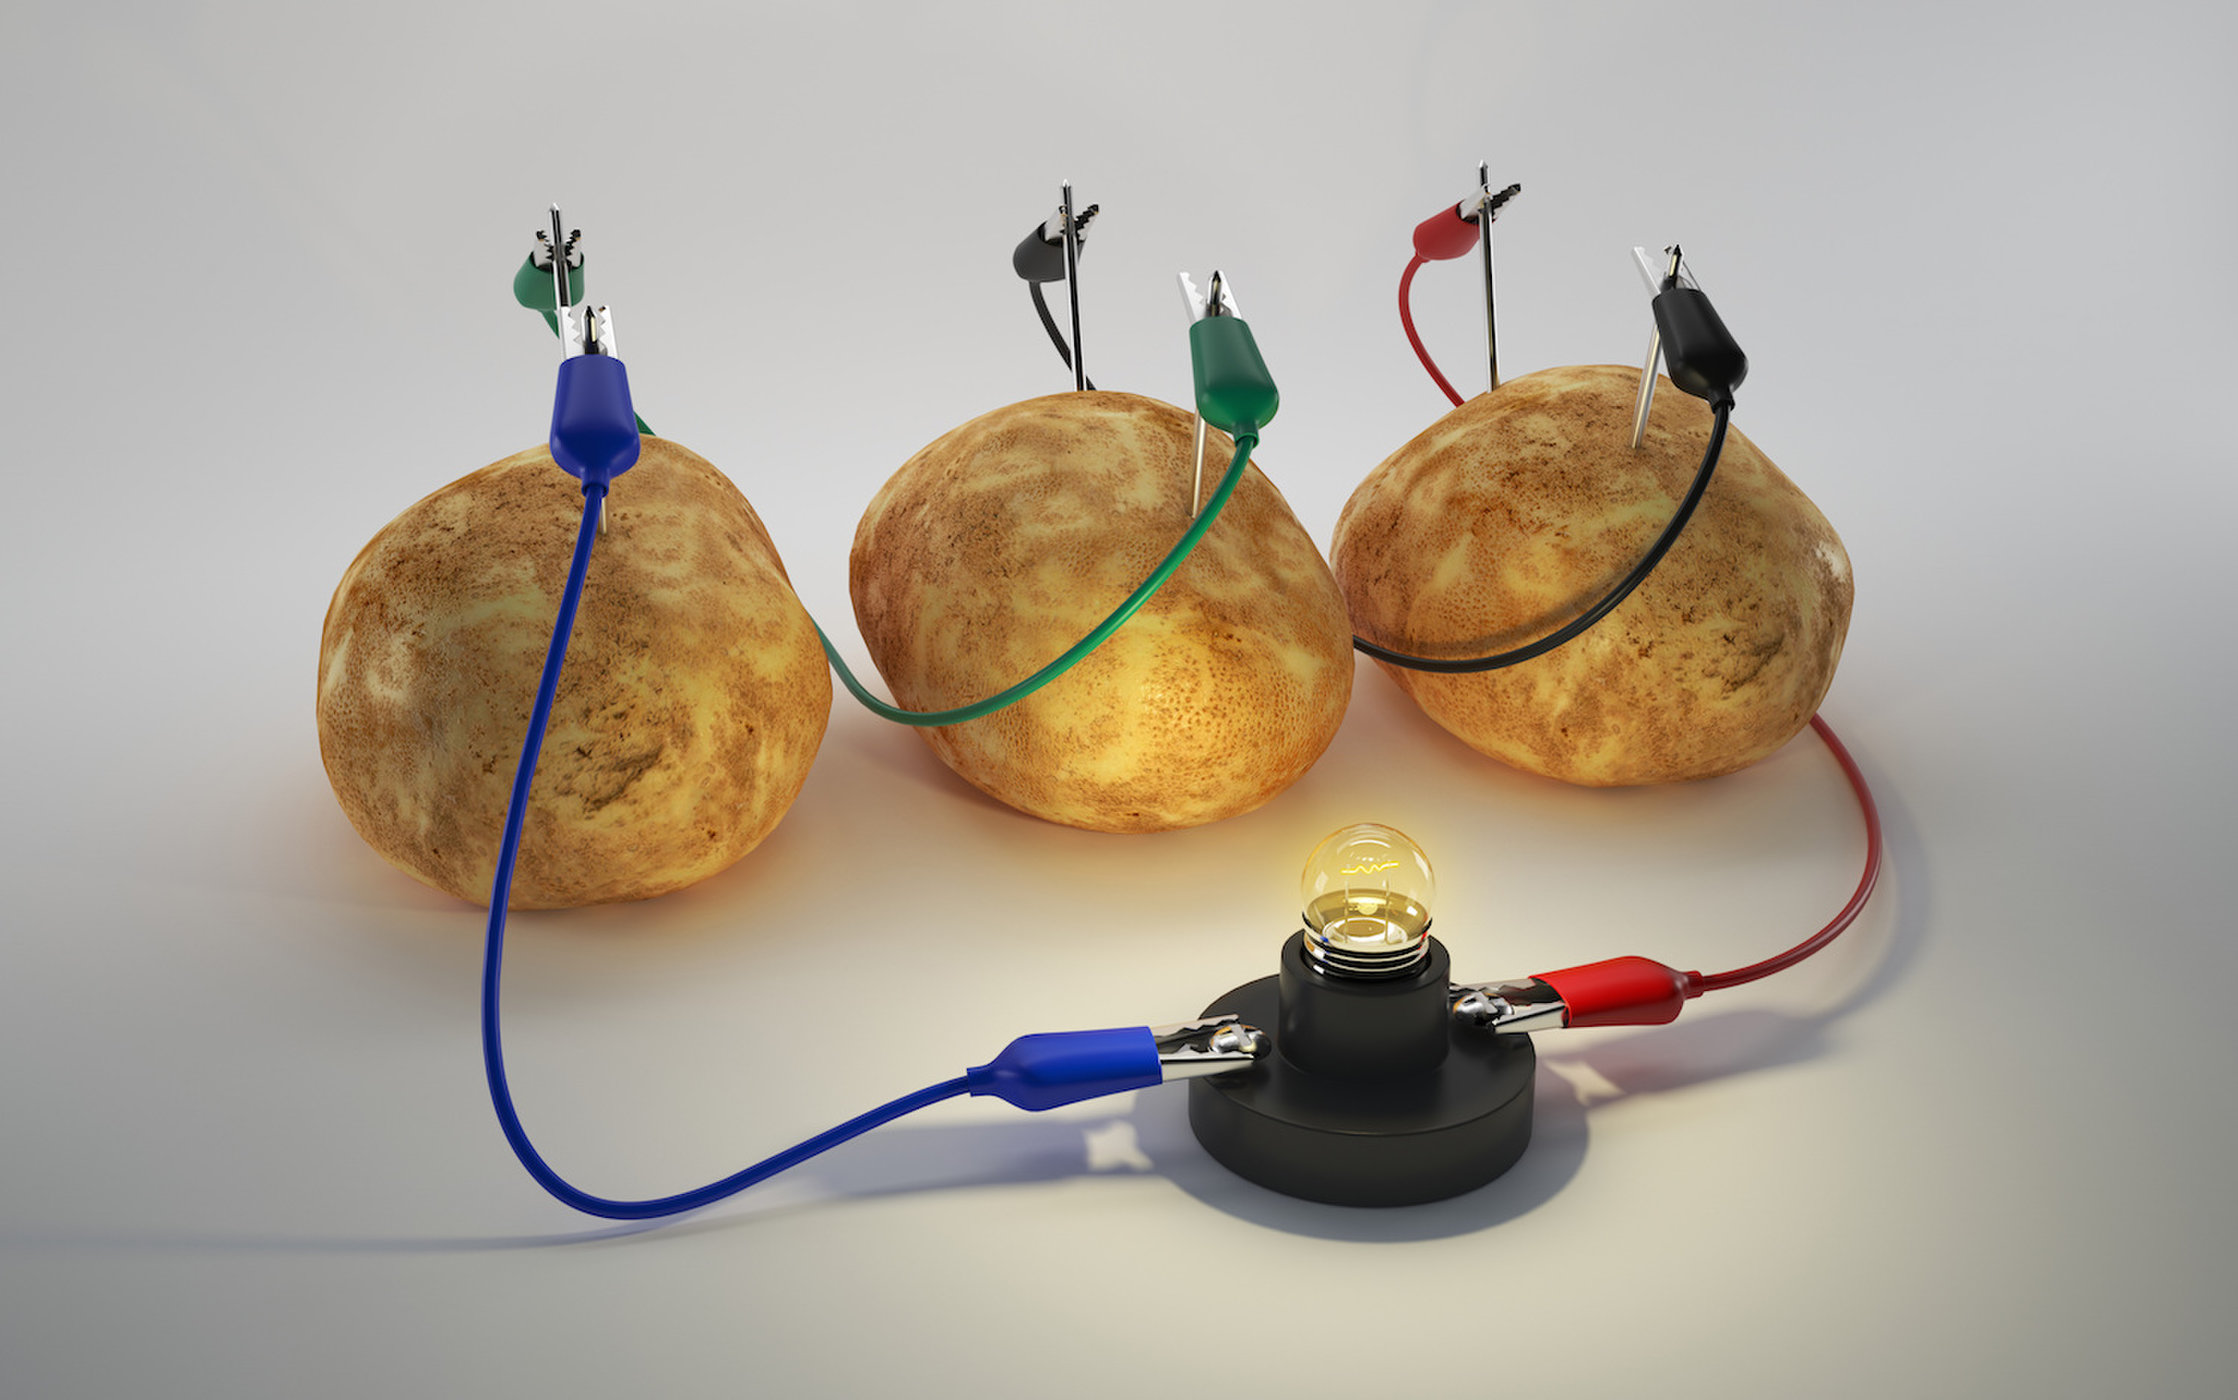
\includegraphics[scale=0.5]{kartoffel.jpg}
		\caption{Typischer Stromkreis.}
	\end{center}
\end{figure}
\noindent
In der Abbildung sehen wir drei Kartoffelbatterien, die mit Dr\"ahten miteinander und mit einer Gl\"uhbirne verbunden sind. Dieser Stromkreis kann als Schaltplan idealisierter Komponenten abstrahiert werden. Hierbei werden irrelevante Eigenschaften der Bausteine des Stromkreises ignoriert und durch idealisierte Bauteile dargestellt. Unser Kartoffelstromkreis wird in folgendem Schaltplan abstrahiert.
\begin{figure}[H]
	\begin{center}
		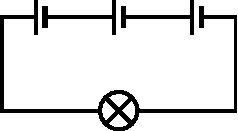
\includegraphics[scale=1]{kartoffel_diagram.pdf}
		\caption{Schaltplan.}
	\end{center}
\end{figure}
\noindent
Wir ignorieren die Farben der Kabeln, die Form der Alligatorklemmen, die Abmessungen der Gl\"uhbirne die L\"ange und Kr\"ummung sowie die Dicke der Kabel. Interessant ist f\"ur uns, was f\"ur Bauteile da sind, also drei Spannungsquellen (Kartoffelbatterien) und ein Verbraucher ( Gl\"uhbirne) und wie diese durch Leiter (Kabel) untereinander verbunden sind.\\
\\
Ein \textbf{Schaltplan} ist ein Netzwerk bestehend aus \textbf{Knoten} und \textbf{elektrischen Bauteilen}, die durch Kanten, welche elektrische Leiter darstellen, miteinander verbunden sind.\\
Jedes Bauteil hat eine feste Anzahl an Anschl\"ussen und ein Leiter endet immer an eineer Seite an einem Anschluss eines Bauteils und an der anderen Seite an einem Knoten oder einem weiteren Anschluss eines Bauteiles.\\
Betrachten wir ein weiteres Beispiel um dies zu illustrieren. 
\begin{figure}[H]
	\begin{center}
		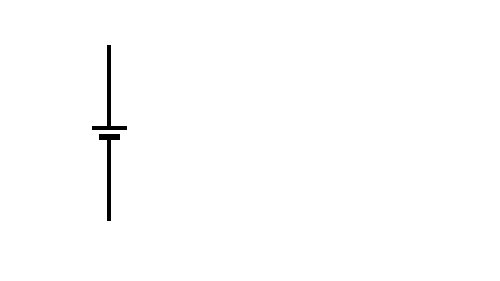
\includegraphics[scale=0.6]{circuit.pdf}
		\caption{Stromkreis.}
	\end{center}
\end{figure}
\noindent
Dieser Schaltplan besteht aus drei Bauteilen, und zwar einer 5 Volt Spannungsquelle (links im Bild), und zwei 100 $\Omega$ Widerst\"ande.
Die geraden Linien sind die Kanten und diese symbolisieren Verbindungen durch elektrische Leiter. Die dicken Punkte sind die Knoten. Knoten sind Ausgangpunkte f\"ur Verzweigungen von Leitern und jede Verzweigung muss in einem Schaltplan \"uber Knoten dargestellt werden.\\
\\
Innerhalb eines elektrischen Netzwerkes k\"onnen zu jedem Zeitpunkt zwei fundamentale Gr\"o\ss{}en gemessen werden. Um diese beiden Gr\"o\ss{}en und ihre Berechnung wird sich das Gro\ss{} diese Kapitel drehen.\\
\\
An jedem Punkt auf jedem der Leiter in einem elektrischen Netzwerk kann eine \textbf{elektrische Stromstr\"arke} gemessen werden. Oft werden wir kurz elektrischer Strom oder nur Strom schreiben.
Eine gute Anschauung f\"ur diese Gr\"o\ss{}e ist eine Fl\"ussigkeit, die \textbf{elektrische Ladung}, die durch ein Rohr, den Leiter, flie\ss{}t. 
Gemessen wird die Menge an Fl\"ussigkeit, die in einer gewissen Zeit, den Rohrquerschnitt beziehungsweise den Punkt im Schaltplan durchflie\ss{}t.\\
\\
Ein Fluss hat auch immer eine Richtung. Da ein Leiter in unserem Schaltplan eine Linie ist, daher nur in eine Richtung Ausdehnung hat, kann dieser Flu\ss{} nur zwei Richtungen haben. Die Richtung wird \"uber das Vorzeichen der Stromst\"arke angegeben. Daher ein elektrischer Strom kann immer nur in Bezug zu einer Messrichtung gemessen werden.\\
\\
Um das positive Vorzeichen auch in Beziehung mit einer Richtung des Leiters (Kante/Linie) setzen zu k\"onnen, muss dem Leiter vor der Messung\footnote{Am Besten beim Design des Schaltplanes.} eine Richtung zugesprochen werden. Die Messung muss dann unter Ber\"ucksichtigung dieser Richtung vollzogen werden.\\
\\
Das Formelsymbol f\"ur den elektrische Strom ist das $I$ und die Ma\ss{}einheit ist das Ampere, abgek\"urzt $A$. 
\\
\\
Die \textbf{elektrische Spannung} ist im Kontrast eine Gr\"o\ss{}e, die von einem beliebigen Punkt zu einem beliebigen anderen Punkt gemessen wird. Wir sehen also, dass auch diese Gr\"o\ss{}e eine Richtung hat. Die elektrische Spannung stellt im Prinzip den Antrieb des elektrischen Stromes zwischen den beiden Punkten dar, was auch erkl\"art warum es eine gerichtete Gr\"o\ss{}e ist. \\
Innerhalb unserer Anschauung der Fl\"ussigkeit, die durch Rohre flie\ss{}t, w\"are diese Gr\"o\ss{}e so etwas wie der Druckunterschied zwischen zwei Punkten. Oder noch einfacher der H\"ohenunterschied zwischen den Rohrabschnitten. Dies legt den Sachverhalt nahe, dass sich nur das Vorzeichen der elektrischen Spannung umdreht wenn man die Reihenfolge der Punkte an denen man misst umdreht.\\
\\
Das Formelsymbol f\"ur die elektrische Spannung ist das $U$ und die Ma\ss{}einheit ist das Volt, abgek\"urzt $V$.\\
\\
Jedem zweipoligen elektrischen Bauteil, daher Bauteil mit zwei Anschl\"ussen, kann eine \textbf{elektrische Leistung} kurz $P$ \"uber die angelgte elektrische Spannung $U$ und die das Bauteil durchflie\ss{}ende elektrische Stromst\"arke $I$ zugeordnet werden.
\begin{equation}
	P = U * I
\end{equation} 
Die elektrische Leistung hat keine besondere Bedeutung f\"ur unsere Diskussion, sollte aber der Vollst\"andigkeit halber erw\"ahnt werden.
\section{Die drei Grundgesetze elektrischer Netzwerke}
In diesem Abschnitt zeigen wir wie wir einen gegebenen Schaltplan in ein Gleichungsystem umwandeln k\"onnen, dass uns erlaubt an jedem Punkt des elektrischen Netzwerkes den Strom und an jedem Paar von Punkten die Spannung zu berechnen.\\
\\
Bevor wir uns den drei Gesetzen widmen, die Strom und Spannung in einem Netzwerk bestimmen, gehen wir kurz auf zwei Vereinfachungen ein, die beim Lesen eines Schaltplanes angenommen werden.\\
\\
Wir nehmen an, dass die Kanten, die Bauteile und Knoten verbinden, den Strom und die Spannung nicht beeinflu\ss{}. Ihre Interpretation soll einzig und allein das darstellen von Verbindungen zwischen Komponenten sein. Strom und Spannungs Abh\"anigkeiten werden allein in die Bauteile gepresst. Wenn man genau sein will h\"atten wir den Schaltplan unseres Kartoffelstromkreises so zeichnen m\"ussen:
\begin{figure}[H]
	\begin{center}
		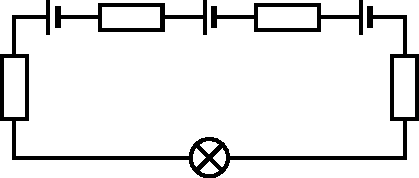
\includegraphics[scale=0.6]{true_kartoffel.pdf}
		\caption{Der wahre Kartoffelschaltplan.}
	\end{center}
\end{figure}
\noindent
Wir sehen, jedem einzelnen Kabel wurde jetzt ein Bauteil zugeordnet, symbolisiert durch Rechtecke. In diesen Schaltsymbolen ist nun der Einflu\ss{} des Kabelmaterials auf Strom und Spannung versteckt.\\
In der Praxis l\"asst man dies aber oft weg, weil der Einflu\ss{} auf das Strom Spannungsverhalten von guten Leitern wie Metall nur sehr klein ist.
\\
\\
Praktisch bedeutet dies f\"ur die Interpretation des Schalplanes, dass wenn wir zwischen zwei Punkten die Spannung bestimmen, der Wert nicht von dem Punkten abh\"angt die man gew\"alt hat, sondern von den Kanten auf denen die Punkte liegen. Daher ist die Spannung zwischen zwei Punkten derselben Spalte im Prinzip Null und wir vergleichen beim Spannungsmessen nicht Punkte sondern ganze Kanten.
\\
\\
\"Ahnliches gilt f\"ur die Interpretation von Knoten, die einzig und allein als Symbold f\"ur Verzweigungen im Netzwerk dienen. Es gilt daher, dass die Spannung zwischen zwei Kanten, die am selben Knoten anliegen gleich Null ist.\\
\\
Kommen wir zur\"uck zu unserer Anschauung des elektrischen Netzwerkes als Rohrwerk durch das eine Fl\"u\ss{}igkeit flie\ss{}t. Hieraus wollen nun das erste unserer Grundgesetze ableiten.
\\
\\
Betrachten wir hierzu eine Verzweigung in einem Rohrwerk. Drei Rohre, Rohr $A$, Rohr $B$ und Rohr $C$ treffen sich in einem Punkt. Es flie\ss{}t nun eine bestimmte Flu\ss{}igkeitsmenge $X$ in einer gegebenen Zeit durch das Rohr $A$ in die Verzweigung. Nachdem das Rohr vollst\"andig mit Fl\"u\ss{}igkeit gef\"ullt ist\footnote{Damit die Anschauung korrekt ist, m\"ussen wir annehmen, dass keine Luft im Rohrwerk ist.} und sich eine Fl\"ussigkeit nicht verdichten l\"asst muss in der selben Zeit in Summe die Menge $X$ aus Rohr $B$ und Rohr $C$ hinausflie\ss{}en.\\
\\
Das gerade beschriebene Konzept nennt sich \textbf{Kontinuit\"atsgesetz} und ist \"uberall dort anzutreffen wo sich Dinge fl\"u\ss{}igkeits\"hnlich verhalten.\\
\\
Zu solchen Dingen z\"ahlen neben Wasser, Benzin und Milch, auch W\"arme und elektrische Ladung in einem Leiter. In der Elektronik nenn man dieses Konzept auch \textbf{Knotenregel}.\\
In unserer Abstraktion eines elektrischen Netzwerkes als Schaltplan bedeutet dies, zum Einen dass die Summe der in einen Knoten oder in ein elektrisches Bauteil flie\ss{}enden Str\"ome gleich der Summe der abflie\ss{}enden Str\"ome ist, und zum Anderen, dass auf einer gegebenen Kante jeder Punkt den selben Strom hat.\\
\\
\textbf{Beispiel}: Nehmen wir einen Knoten mit zwei zuflie\ss{}enden Kanten und einer wegflie\ss{}enden Kante.
\begin{figure}[H]
	\begin{center}
		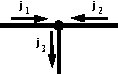
\includegraphics[scale=2]{flow.pdf}
		\caption{Str\"ome.}
	\end{center}
\end{figure}
\noindent
Der Flu\ss{} bezieht sich dabei auf die vor der Messung festgelegte Referenz Flu\ss{}richtung jeder Kante. Ein positiver Strom bedeutet also Flu\ss{} entlang der Richtung, w\"ahrend ein negativer Strom der Richtung entgegengesetzt ist. In diesem Fall besagt das Kontinuit\"atssatz:
\begin{equation}
i_1 + i_2 = i_3
\end{equation}
\paragraph{\"Ubungsbeispiel:} Formuliere das Kontinuit\"atsgesetz f\"ur die folgende Anordnung:
\begin{figure}[H]
	\centering{
		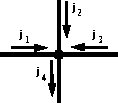
\includegraphics[scale=2]{aufgabe.pdf}
		\caption{Aufgabe.}
		\label{fig:circuit}
	}
\end{figure}
\noindent
Als n\"achstes widmen wir uns dem zweiten Grundgesetz. So wie die Knotenregel die Struktur des Netzwerkes in Verbindung mit den elektrischen Str\"omen setzt, so verbindet dieses die Netzstruktur mit den Spannungen.\\
\\
Zur Motivation des neuen Gesetzes gehen wir wieder zur\"uck zur Anschaung des fl\"ussigkeitsdurchflossenen R\"ohrensystems. Wir haben ja bereits in diesem Bilde die Spannung als H\"ohenunterschied der Rohrabschnitte beschrieben.\\
\\
Damit diese Anschauung der Spannung aber mit unserer Erfahrung zu H\"ohen- unterschieden \"ubereinstimmt, muss gelten, dass sie unabh\"angig vom Weg ist, der zur\"uckgelegt wurde um Teilabschnitte zu vermessen. Zur Erkl\"arung: Wir machen uns zusammen auf, einen Berg zu besteigen. Dabei starten wir beide am selben Punkt, sagen wir dem Parkplatz am Fu\ss{} des Berges. Anschlie\ss{}end wandern wir auf unterschiedlichen Pfaden den Berg hinauf und machen zwischendurch Halt an jeweils verschiedenen Bergh\"utten. Am Ende treffen wir uns beide am Gipfel. Messen wir beide bei der Pause in der H\"utte den H\"ohenunterschied zum Parkplatz und dann am Gipfel den H\"ohenunterschied zu der H\"utte, an der wir Pause gemacht haben, dann muss die Summe dieser Werte f\"ur uns beide gleich sein. Als Konsequenz k\"onnen wir offensichtlich eine absolute H\"ohe definieren als den H\"ohenunterschied zum Parkplatz (oder irgendeinem anderen festen Punkt). Jeder H\"ohenunterschied zwischen einem Punkt $A$ und einem Punkt $B$ ist dann genau gleich der Differenz der absoluten H\"ohe am Punkt $B$ minus der am Punkt $A$.\\
\\
Dieses Prinzip, dass eine Eigenschaft eines Weges, die nur abh\"angig vom Anfangs und Endpunkt des Weges ist, eine absolute Eigenschaft f\"ur jeden Punkt definiert, ist ein wichtiges Konzept aus der Potentialtheorie, einem Teilgebiet der Mathematik und hat in der Elektronik eine analoge Bedeutung.
\\
\\
In einem Schaltplan gilt dieses Konzept ganz analog f\"ur die elektrische Spannung.
Man w\"ahle zwei Kanten im Schaltplan und einen Pfad zwischen den beiden Kanten. Wenn man an der ersten Kante startet und den Pfad durchwandert und dabei die Spannungen zwischen aufeinanderfolgenden Kanten misst, dann ergibt die Summe der Spannungen sobald man bei der letzten Kante ankommt dieselbe Spannung die man zwischen der ersten und letzten Kante misst. Insbesondere bedeutet dies, dass f\"ur jeden geschlossenen Pfad die Summe dieser Spannungen Null sein muss.
Diese Regel nennt man die \textbf{Maschenregel}, wobei Maschen sich auf jene geschlossenen Pfade im Schaltplan bezieht.
\begin{theorem}
	Gegeben sei ein Schaltplan, dann gilt die Maschenregel genau dann wenn es eine Funktion $\psi$ gibt, die jeder Kante einen Zahlenwert zuordnet, sodass die gemessene Spannung zwischen der Kante $x$ zur Kante $y$ genau die Differenz $\psi(y)-\psi(x)$ ist.
\end{theorem}
\noindent
Eine solche Funktion $\psi$ der Kanten nennen wir eine \textbf{Potentialfunktion} und wir werden anstelle der Maschenregel immer von der Existenz einer Potentialfunktion ausgehen, da dies eine einfachere Analyse elektrischer Netzwerke erlaubt.
\begin{corollary}
	Eine Potentialfunktion eines Schaltplans $X$ ist bis auf eine additive Konstante eindeutig festgelegt, daher falls $\psi$ eine Potentialfunktion von $X$ ist und $c$ ein reele Zahl, dann ist $\psi + c$ auch eine Potentialfunktion von $X$.
\end{corollary}
\noindent
Bisher haben wir den Einflu\ss{} der Struktur des Schalplans, also des Netzwerkes an Verbindungen, behandelt. Der Einflu\ss{} der elektrischen Bauteile selbst auf Spannungen und Stromst\"arken wurde bislang ausgelassen. Dies stellt das dritte Gesetz elektrischer Netzwerke dar.\\
Ein elektrisches Bauteil hat eine bestimmte feste Anzahl von Anschl\"ussen oder Pole an welche elektrische Leiter/Kanten befestigt/geklemmt werden k\"onnen. Das Verhalten eines elektrischen Bauteiles wird durch die \textbf{Strom-Spannungs-Kennlinie} oder allgemeiner \textbf{Charakteristik} kurz $\Phi$ bestimmt. Sie legt fest welche Str\"ome zwischen den Anschl\"ussen bei gegebenen Spannungen an den Anschl\"ussen erlaubt sind. Die allgemeinste abstrakte Definition des Konzeptes ist:
\begin{definition}
	Eine Charakteristik $\Phi$ eines elektrischen Bauteiles mit $N$ Anschl\"ussen ist eine Teilmenge des $2 * (N - 1)$-dimensionalen Raumes. Wobei die ersten $N - 1$ Komponenten Potentialwerte an den Anschl\"ussen repr\"asentieren und die restlichen Komponenten die entsprechenden Strom- st\"arken.\footnote{Die Stromst\"arken sind bereits wegen der Knotenregel durch $N - 1$ Werte  festgelegt. Da Potentiale genauso wegen ihrer Eindeutigkeit bis auf eine additive Konstante.}
\end{definition}
\noindent
Die allgemeine Form einer Charakteristik eines $N$-poligen Bauteiles ist eine Gleichung oder ein Gleichungssystem, deren Variablen die $N-1$ Potentialwerte und $N-1$ Stromstr\"arken sind und damit eine Teilmenge festlegt. \\Wir werden bis auf wenige Ausnahmen aber davon ausgehen, dass die Charakteristik, hier im Fall eines zweipoligen Bauteiles, eine Funktion der Form
\begin{equation*}
	I = \Phi(U)
\end{equation*}
ist. Also eine Zuordnung die den $N-1$ Potentialwerten eindeutig die $N-1$ Str\"ome zuordnet. \\
\\
Die Charakteristik eines Bauteiles kann direkt gemessen werden (zb.: mit einem Oszilloskop; siehe Anhang) oder typischerweise im vom Hersteller zur Verf\"ungung gestellten Datenblatt des elektrischen Bauteiles.
\begin{figure}[H]
	\begin{center}
		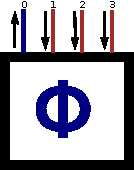
\includegraphics[scale=1]{charakter.pdf}
	\end{center}
	\caption{Charakteristik eines mehrpoligen Bauteiles.}
\end{figure}
\noindent
Die Abbildung (4.4) zeigt eine M\"oglichkeit die Charakteristik eines vierpoligen elektrisches Bauteiles darzustellen. Man beachte, dass eine der Anschl\"usse, Nummer 0, als Ausgang deklariert ist und diesem das Referenzpotential Null zugeordnet wird, sowie eine abflie\ss{}ende Stromst\"arke, die gleich der Summme der an den Eing\"angen 1, 2 und 3 zuflie\ss{}enden Str\"omen ist. Die Charakteristik $\Phi$ hat drei Komponenten f\"ur jeden Ausgang.
\begin{align} 
\begin{split}
\Phi = (\Phi^1, \Phi^2, \Phi^3)\\
i_1 = \Phi^1(\phi_1,\phi_2,\phi_3)\\
i_2 = \Phi^2(\phi_1,\phi_2,\phi_3)\\
i_3 = \Phi^3(\phi_1,\phi_2,\phi_3)\\
\end{split}
\end{align}
\noindent
Eine \textbf{ideale elektrische Spannungsquelle} ist ein zwei poliges elektrisches Bauteil von dem unabh\"angig von der abgenommenen Stromst\"arke eine konstante Spanung abgenommen werden kann. 
\begin{figure}[H]
	\begin{center}
		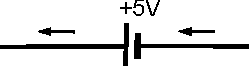
\includegraphics[scale=1]{ideal.pdf}
		\caption{Schaltsymbol ideale Spannungsquelle.}
	\end{center}
\end{figure}
\noindent
Beachte die Pfeile in der obigen Abbildung, die nicht Teil des eigentlichen Schaltsymbols sind, sondern eine Konvention der Flu\ss{}richtung anzeigen. Die Konvention besagt, dass die l\"angere der beiden paralellen Linien als der Ausgang angesehen wird.\\
\\
Die Strom- Spannungs- Kennlinie einer 5V Spannungsquelle sieht folgenderma\ss{}en aus.
\begin{figure}[H]
	\centering{
		\resizebox{65mm}{!}{\input{ideal_spannung.pdf_tex}}
		\caption{Charakteristik Spannungsquelle.}
		\label{fig:circuit}
	}
\end{figure}
\noindent
Dies ist ein Beispiel bei dem die Charakteristik keine Funktion ist sondern man sich zur Beschreibung die allgemeinere Form, eine Gleichung, bedienen muss: $U=5$.\\
\\
In unserer Fl\"u\ss{}igkeitsanalogie des elektrischen Stromes w\"are dies eine Pumpe mit konstantem Druck.\\
Reale Spannungsquellen, wie Zink/Kohle Batterien oder Lithium- Ionen- Akkumulatoren haben nur in einem sehr kleinen Stromst\"arke Bereich eine derartige vertikale Charakteristik.\\
\\
Als n\"achstes Bauteil lernen wir die Gl\"uhbirne kennen. Eine Gl\"ubirne ist ein zweipoliges Bauteil, das Licht erzeugt wenn es mit Strom durchflossen wird.
\begin{figure}[H]
	\begin{center}
		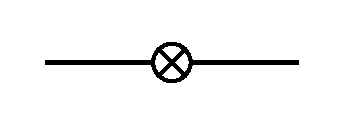
\includegraphics[scale=1]{gluh.pdf}
		\caption{Schaltsymbol Gl\"uhbirne.}
	\end{center}
\end{figure}
\noindent
Eine elektrische Gl\"uhbirne hat eine parabolische Charakteristik.
\begin{figure}[H]
	\centering{
		\resizebox{65mm}{!}{\input{gluhbirne.pdf_tex}}
		\caption{Charakteristik Gl\"uhbirne.}
		\label{fig:circuit}
	}
\end{figure}
\noindent
Man bemerke hier, dass im Gegensatz zur Spannungsquelle, hier die Charakteristik durch den Ursprung $(0,0)$ geht. Es ist leicht zu sehen, dass Quellen diese Eigenschaft haben m\"ussen um ihre Funktion zu erf\"ullen. Au\ss{}erdem ist die Charakteristik symmetrische im Sinne von 
\begin{equation*}
	\Phi(-U) = - j.
\end{equation*}
Daher sie sieht gleich aus wenn man an der $x-$Achse und anschlie\ss{}end and der $y-$Achse spiegelt. Bei Charakteristiken mit dieser Symmetrie ist es egal welchen der Pole man als Eingang und welchen als Ausgang z\"ahlt. Ein derartiges Bauteil nennt man auch ungerichtet. \footnote{In der Regel erkennt man, dass ein Bauteil ungerichtet ist wenn das Schaltsymbol symmetrisch ist.}
\\
\\
\paragraph{\"Ubungsbeispiel:} \"Uberzeuge dich davon, dass es tats\"achlich keinen Unterschied macht welcher Pol als Eingang gesehen wird. 
\subsection{Zusammenfassung}
Gegeben sei ein elektrischer Stromkreis bestehend aus Knoten und elektrischen Bauteilen verbunden durch Kanten, welche elektrische Verbindungen beziehungsweise Leiter darstellen.
\\
\\
Hier ein Beispiel eines abstrakten elektrischen Stromkreises. 
\begin{figure}[H]
	\begin{center}
		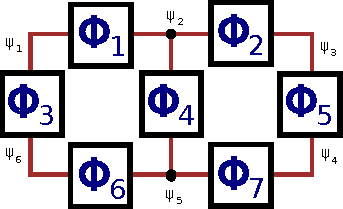
\includegraphics[scale=1]{_abstract.pdf}
	\end{center}
\end{figure}
\noindent
Die K\"astchen symbolisieren die elektrischen Bauteile, mitsamt ihrer Charakteristik $\Phi$. Die Kanten wurden zur besseren Lesbarkeit rot angef\"arbt. In der Mitte gibt es oben und unten zwei Knoten, wieder symbolisiert durch einen dicken schwarzen Punkt.\\
Gesucht ist nun eine Potentialfunktion $\psi$, die jeder Kante einen Potentialwert zuordnet, und somit jedem elektrischen Bauteil eindeutig die elektrische Spannung an jedem der Paare von Eing\"agen.\\
Kanten, welche direkt \"uber Knoten verbunden sind, haben den selben Potentialwert, da wir ja festgelegt haben, dass zwischen darauf liegenden Punkten die Spannung Null ist.\\
Somit haben wir sechs Bereiche an denen die Potentialfunktion konstanten Wert hat; im Bild angezeigt durch $\{\psi_1, \psi_2, \psi_3, \psi_4, \psi_5, \psi_6\}$. 
\begin{figure}[H]
	\begin{center}
		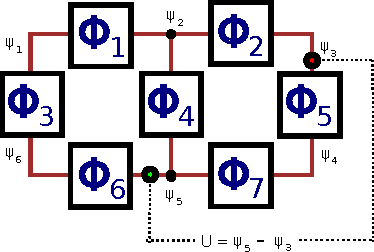
\includegraphics[scale=1]{potent.pdf}
	\end{center}
\end{figure}
\noindent
Hier wird gezeigt wie die Spannung $U$ von einem Punkt bei $\psi_3$ zu einem Punkt an $\psi_5$ gemessen und mit Hilfe der Potentialfunktion berechnet werden kann\\
\\
Als n\"achstes betrachten wir die elektrischen Stromst\"arken die innerhalb des Stromkreises auftreten und die Flu\ss{}richtungen: 
\begin{figure}[H]
	\begin{center}
		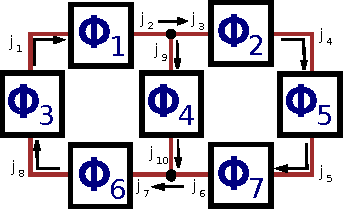
\includegraphics[scale=1]{laminar.pdf}
	\end{center}
\end{figure}
\noindent
Die Charakteristiken der elektrischen Bauteile wiederum legen f\"ur jede Kante eindeutig die elektrische Stromst\"arke fest. Bedenke dabei, dass immer der zuflie\ss{}ende Strom in unserer Definition einer Charakteristik betrachtet wird und immer in Bezug gesetzt zur Differenz des Potential des Einganges der betrachtet wird minus dem Potentials am Ausgang. Zus\"tzlich vergess nicht, dass die Flu\"ss{}richtungen im Netzwerk nicht mit den vorher f\"r die Bauteil Anschl\"usse festgelegten Richtungen \"ubereinstimmen muss.\\
\begin{align} 
\begin{split}
j_1 = \Phi_1(\psi_1 - \psi_2)\\
j_3 = \Phi_2(\psi_2 - \psi_3)\\
j_8 = \Phi_3(\psi_6 - \psi_1)\\
j_9 = \Phi_4(\psi_2 - \psi_5)\\
j_4 = \Phi_5(\psi_3 - \psi_4)\\
j_7 = \Phi_6(\psi_5 - \psi_6)\\
j_5 = \Phi_7(\psi_4 - \psi_5)
\end{split}
\end{align}
Wir sehen, dass viele der Stromst\"arken bereits direkt \"uber die Potentialfunktion und die Charakteristiken gegeben sind. \\
Die Knotenregel erlaubt es uns den Rest der Str\"ome zu bestimmen. Wir k\"onnen diese direkt aus dem Bild ablesen. Beachte die jeweilige Flu\ss{}richtung.
\begin{align} 
\begin{split}
j_1 = j_2\\
j_2 = j_3 + j_9\\
j_3 = j_4\\
j_4 = j_5\\
j_5 = j_6\\
j_9 = j_{10}\\
j_7 = j_8\\
j_8 = j_1\\
j_{10} + j_6 = j_7
\end{split}
\end{align}
Wir sehen also, dass wenn eine Potentialfunktion gegeben ist, bereits alle me\ss{}baren Gr\"o\ss{}en im Stromkreis, daher Spannungen und Stromst\"arken, eindeutig bestimmt sind.\footnote{Eindeutig nur falls die Charakteristiken eindeutige Zuordnungen sind.}\\
\\
Kombinieren wir, die aus der Knotenregel abgeleitet Gleichungen (4.4), und die Gleichungen (4.3), die aus den Charakteristiken  bestimmt wurden, so erhalten wir ein Gleichungssystem dessen Variablen die m\"glichen Werte der Potentialfunktion des Stromkreises darstellen. Dies erm\"oglicht es uns die zu einem Stromkreis geh\"orende unbekannte Potentialfunktion zu bestimmen. Wir werden das im Detail im Kapitel \"uber lineare Stromkreise zeigen.
\\
\\
Abschlie\ss{}end ist zu bedenken, dass wir eine Reihe von Idealisierungen in unserer Beschreibung getroffen haben. Ein wesentlicher Aspekt dabei ist, dass wir von einem statischen elektrischen Stromkreis ausgehen. Weder die Stromst\"arke noch die Spannung sind abh\"angig von der Zeit. In einem realen elektrischen Stromkreis, braucht die Spannung so wie der Strom eine gewisse Zeit bis er bei Anschlu\ss{} der Spannungsquelle von der einen Seite des Stromkreises zur anderen gewandert ist. Zus\"atzlich gibt es elektrische Bauteile, die bisher noch nicht erw\"ahnt wurden, die eine interne Dynamik haben, daher zu einem Stromkreis mit zeitabh\"angigen Strom und Spannungswerten f\"uhren.
Ein weiterer nicht unwesentlicher Aspekt ist der Einflu\ss{} der Umwelt auf den elektrischen Stromkreis. Hierzu geh\"oren die Temperatur, elektromagnetische Felder, Feuchtigkeit etc.
Auf der anderen Seite werden einige von diesen Umwelteigenschaften, wie Temperatur und Elektromagnetismus von unserem Stromkreis beeinflu\ss{}t. Normalerweise wird versucht solche Einfl\"u\ss{}e so klein wie m\"oglich zu halten, aber oft l\"asst es sich nicht vermeiden und darf nicht vergessen werden.
\section{Lineare elektrische Netzwerke}
Eine wichtige Erkenntnis in der Elektronik ist das Ohm'sche Gesetz, welches besagt, dass bei kleinen Stromst\"arken und Spannungen die Charakteristiken von vielen Materialen ann\"ahernd linear sind.
\begin{figure}[H]
	\centering{
		\resizebox{65mm}{!}{\input{widerstand.pdf_tex}}
		\caption{Charakteristik Widerstand.}
		\label{fig:circuit}
	}
\end{figure}
\noindent
Ein elektrisches Bauteil mit linearer Charakteristik gehorcht dem Ohm'schen Gesetz; Wenn wir nun die Charakteristik $\Phi$ des Bauteils als lineare Funktion schreiben, erhalten wir eine Form des Ohm'schen Gesetzes.
\begin{equation}
I = \Phi(U) = G * U
\end{equation}
Wobei $G$, also die Steigung der Strom/Spannungskurve, \textbf{elektrische Leitf\"ahigkeit} genannt wird.\\
Die gewohnte Form des Ohm'schen Gesetzes erhalten wir aber \"uber die  Spannungs/Strom Kurve:
\begin{equation}
U = I * R
\end{equation}
\noindent
Der Wert $R$, also die Steigung der Spannungs/Strom Kurve, ist bekannt als elektrischer Widerstand und wird gemessen in Ohm kurz $\Omega$.
Es gilt nat\"urlich der Zusammenhang
\begin{equation}
G = \frac{1}{R}
\end{equation}
zwischen Widerstand und Leitf\"ahigkeit.
\\
\\
Das elektrische Bauteil assoziiert mit dem Ohm'schen Widerstand ist der Widerstand mit dem Schaltsymbol.
\begin{figure}[H]
	\begin{center}
		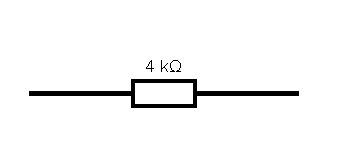
\includegraphics[scale=1]{widder.pdf}
		\caption{Schaltsymbol 4000 $\Omega$ Widerstand.}
	\end{center}
\end{figure}
\noindent
Eine lineare Funktion erf\"ullt die selbe Symmetrie wie die Gl\"uhbirne (Abbildung 4.8). die Flu\ss{}richtungen k\"onnen daher beliebig gew\"ahlt werden.\\
\\
Ein elektrischer Widerstand stellt einen quantitativen Zusammenhang zwischen Strom und Spannung her und kann wie der Name schn sagt als Widerstand des Bauteiles gegen die Verursachung von elektrischem Strom durch eine gegebene elektrische Spannung angesehen werden.\\
Innerhalb unserer Anschauung der Fl\"ussigkeit, die sich durch R\"ohren bewegt, w\"are dies so etwas wie ein Gewebe oder ein por\"oses Material, durch die die Fl\"u\ss{}igkeit mit Druck gepresst werden muss.
\subsection{Reihen und parallele Schaltungen}
Bestimmte h\"aufig auftretende Teilstrukturen elektrischer Stromkreise werden als elektrische Bauteile abstrahiert. Hierbei errechnet sich, abh\"angig von der Teilstruktur die Charakteristik des abstrahierten Bauteiles aus den Charakteristiken der darin enthaltenen Bauteile.\\
\\
Gegeben sei eine Teilstruktur bestehend aus mehreren zweipoligen elektrischen Bauteilen, die nacheinander geschaltet sind, eine so genannte \textbf{Reihenschaltung}.
\begin{figure}[H]
	\begin{center}
		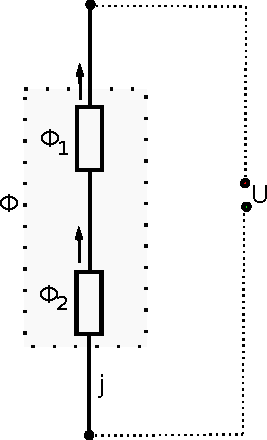
\includegraphics[scale=0.75]{reihe.pdf}
		\caption{Reihenschaltung.}
	\end{center}
\end{figure}
\noindent
Hier haben wir ein Beispiel mit zwei Bauteilen, mit Charakteristiken $\Phi_1$ und $\Phi_2$. Man beachte das gepunkte Rechteck um die beiden Bauteile. Dies soll unser zusammengesetztes Bauteil darstellen, zusammen mit dessen Charakteristik $\Phi$. Gesucht ist $\Phi$. Wir wissen, dass Wegen der Knotenregel die Stromst\"arke \"uberall im Stromkreis gleich sein muss, weil es ja keine Verzweigung gibt. Wir setzten den Potentialwert der oberen Kante auf Null, was wir ja d\"urfen, weil das Potential immer bis auf eine Konstante nur eindeutig ist und daher ein Potentialwert frei gew\"ahlt werden darf. Die untere Kannte hat damit laut Abbildung den Potentialwert $U$. Es verbleibt der Potentialwert, nennen wir ihn $u'$ der verbleibenden Kante zwischen den Bauteilen zu bestimmen. \\Dieser muss erf\"ullen, dass $\Phi_1(u' - 0)=\Phi_1(u') = j$ ist und das $\Phi_2(U - u') = j$ ist. Wenn wir zu einem gegebenen $U$ das $u'$ und damit $j$, da $j = \Phi_1(u')$ bestimmen k\"onnen haben wir unsere Charakteristik $\Phi$ gefunden. Diese Gleichungsystem ist im allgemeinen nicht linearen Fall das Best, dass wir tun k\"onnen. Nehmen wir an $\Phi_1$ und $\Phi_2$ sind linear, daher $\Phi_1(u) = u / R_1$ und $\Phi_2(u) = u / R_2$. Wobei $R_1$ und $R_2$ die Widerst\"ande der Bauteile sind.\\
Das Problem vereinfacht sich stark und es ist leicht zu zeigen, dass $\Phi(u) = u / R$ ist, wobei 
\begin{equation}
	R = R_1 + R_2.
\end{equation}
\noindent
\paragraph{\"Ubungsbeispiel:} Zeige die G\"ultigkeit von 4.9.
\\
\\
Gegeben sei eine Teilstruktur bestehend aus mehreren zweipoligen elektrischen Bauteilen, die nebeneinander geschaltet sind, eine so genannte \textbf{Paralellschaltung}. In der folgenden Abbildung sehen wir ein Beispiel mit zwei paralell geschalteten Bauteilen.
\begin{figure}[H]
	\begin{center}
		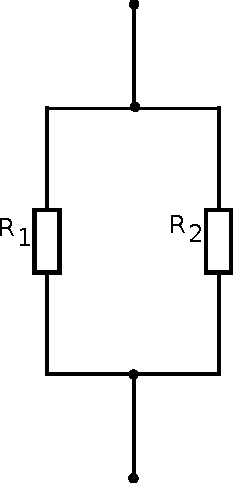
\includegraphics[scale=0.75]{Parallel.pdf}
		\caption{Paralellschaltung.}
	\end{center}
\end{figure}
\noindent
Wie im letzten Beispiel haben wir hier zwei Bauteile mit Charakteristiken $\Phi_1$ und $\Phi_2$, sowie ein gepunktetes Rechteck um diese, welches das zusammengesetzte Bauteil symbolisiert, dessen Charakteristik $\Phi$ wir suchen. Es liegt eine Spannung von $U$ zwischen dem oberen und dem unteren Punkt an und wir suchen die zugeh\"orige Stromst\"arke $j$. Wir legen wieder fest, dass oben, daher der gesamte durch den Knoten verbundene Bereich oberhalb der Bauteile, den Potentialwert Null hat und analog unten der Potential wert $U$. Nun liegt an beiden Bauteilen dieselbe Spannung $U$ an, daher produzieren sie jeweils auf ihre Leiterverzweigung den zugeh\"origen Strom $j_1 = \Phi_1(U)$ und $j_2 = \Phi_2(U)$. Nach der Knotenregel ergibt sich $j = j_1 + j_2$. Es gilt also 
\begin{equation}
	\Phi(U) = \Phi_1(U) + \Phi_2(U)
\end{equation}
Es ist leicht zu sehen, dass wenn wir annehmen, dass unsere Bauteile lineare Charakteristik haben, daher $\Phi_1(U) = U / R_1$ und $\Phi_2(U) = U / R_2$ ist, dann ist $\Phi(U) = U / R$, wobei $R$ sich errechnet aus
\begin{equation*}
	\frac{1}{R} = \frac{1}{R_1} + \frac{1}{R_2}
\end{equation*}
\subsection{Lineare Systeme}
Die Gleichungen in (4.3) reduzieren sich im Fall von Bauteilen mit linearer Charakteristik zu linearen Gleichungen und mit Hilfe von (4.4) erhalten wir ein lineares Gleichungssystem, das mit klassischen Methoden wie dem Gau\ss{}schen Eliminationsverfahren gel\"ost werden kann. \\Wir zeigen in diesen Abschnitt wie dies an einem konkreten Beispiel funktioniert und dass wir im Fall von zweipoligen linearen Bauteilen immer eine eindeutige L\"osung haben.\\
\\
Gegeben sei ein elektrischer Stromkreis bestehend aus einer quadratischen Anordnung von Widerst\"anden. Die Kanten des Quadrats sind Widerst\"ande, die Ecken sind Knoten. Eine der Diagonalen ist ein Widerstand, die Andere ist eine ideale Spannungsquelle.
\begin{figure}[H]
	\begin{center}
		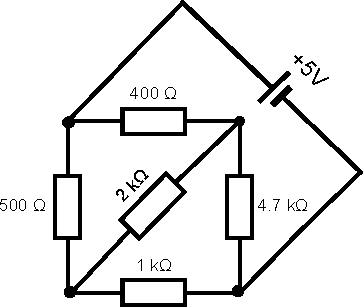
\includegraphics[scale=0.8]{stromkreis_1.pdf}
		\caption{Beispiel.}
	\end{center}
\end{figure}
\noindent
Wir starten mit unserer Analyse des Stromkreises indem wir f\"ur jede Kante eine Vorzugsrichtung ausw\"ahlen und die zugeh\"origen Str\"ome benennen. Die an der Spannungsquelle liegenden Kanten haben bereits eine Vorzugsrichtung (4.5), und f\"ur alle an Widerst\"ande grenzenten Kanten, kann die Flu\ss{}richtung beliebig gew\"ahlt werden (4.10), solange beachtet wird, dass jeder Widerstand eine zuflie\ss{}ende und eine abflie\ss{}ende Kante haben muss.
\begin{figure}[H]
	\begin{center}
		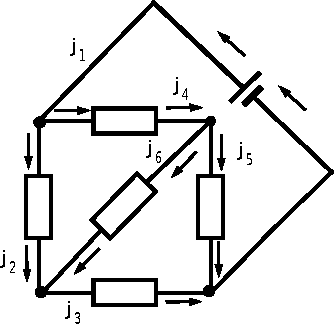
\includegraphics[scale=0.8]{stromkreis_2.pdf}
		\caption{Str\"ome und Richtungen.}
	\end{center}
\end{figure}
\noindent
Um ein wenig mit den Variablen zu sparen, haben wir hier beiden an ein Bauteil geschlossenen Kanten denselben Strom zugeordnet, weil sie ja laut Knotenregel ohnehin gleich sind.\\
\\
Als n\"achstes ordnen wir jedem durch Knoten verbundenen Bereich von Kanten und einzelnen nicht an Knoten grenzende Kanten eine Potentialvariable zu. Die Potentialvariablen stehen f\"ur die unbekannten Potentialwert an den entsprechenden Bereichen.
\begin{figure}[H]
	\begin{center}
		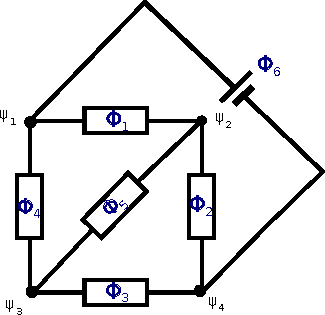
\includegraphics[scale=0.8]{stromkreis_3.pdf}
		\caption{Potentialvariablen.}
	\end{center}
\end{figure}
\noindent
Anstelle von Spannungswerten bei der Spannungsquelle und Widerstandswerten bei den elektrischen Widerst\"anden haben wir $\Phi_x$ f\"ur die Charakteristiken der Bauteile geschrieben. Dies geschah damit wir zu Anfangs im selben Schema wie zuvor arbeiten. \\
\\
Die Charakteristiken geben uns non folgende Gleichungen.
\begin{align} 
\begin{split}
\psi_1 - \psi_4 = 5V\\
j_2 = \Phi_4(\psi_1 - \psi_3) = \frac{\psi_1 - \psi_3}{500\Omega}\\
j_3 = \Phi_3(\psi_3 - \psi_4) = \frac{\psi_3 - \psi_4}{1000\Omega}\\
j_4 = \Phi_1(\psi_1 - \psi_2) = \frac{\psi_1 - \psi_2}{400\Omega}\\
j_5 = \Phi_2(\psi_2 - \psi_4) = \frac{\psi_2 - \psi_4}{4700\Omega}\\
j_6 = \Phi_5(\psi_2 - \psi_3) = \frac{\psi_2 - \psi_3}{2000\Omega}\\
\end{split}
\end{align}
Beachte hierbei die erste Gleichung, welche wir erhalten da sich wie schon gezeigt die Charakteristik der idealen Spannungsquelle nicht als Funktion schreiben l\"asst. Links stehen die Stromst\"arken; in der Mitte dann die Charakteristik als Funktionensymbol und rechts dann die Definition der linearen Charakteristik ausgeschrieben. Wir sehen, dass es keine Gleichung f\"ur $j_1$ gibt, aber dies wird sich \"andern sobald wir die Knotenregeln aufschreiben.\\
\\
Wir wissen bereits, dass Potentialfunktionen immer nur bis auf eine Konstante festgelegt sind. Das bedeutet wir k\"onnen einen der Potentialwerte frei w\"ahlen und es empfliehlt sich bei nur einer Spannungsquelle den Minuspol auf Null zu setzen. In unserem Fall ist das $\psi_4$. Man sagt auch diese Kante ist \textbf{Erde} und man kann diesen Sachverhalt im Schaltplan folgenderma\ss{} darstellen.
\begin{figure}[H]
	\begin{center}
		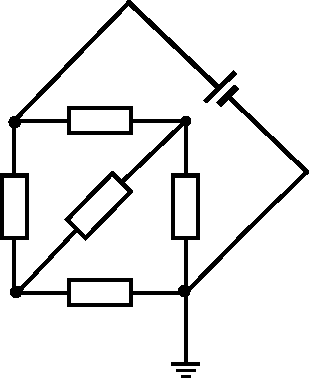
\includegraphics[scale=0.8]{erde.pdf}
		\caption{Erde.}
	\end{center}
\end{figure}
\noindent
Sobald wir $\psi_4 = 0$ gesetzt haben folgt aus (4.11), dass $\psi_1 = 5V$ ist. Wir haben also nur zwei Unbekannte $\psi_2$ und $\psi_3$, welche im weiteren Verlauf dieser Analyse noch eindeutig bestimmt werden.\\
\\
Als n\"achstes kommen wir zu den Gleichungen, die aus der Knotenregel resultieren.
\begin{align} 
j_1 = j_2 + j_4\\
j_2 + j_6 = j_3\\
j_3 + j_5 = j_1\\
j_4 = j_6 + j_5
\end{align}
Die unbekannten Potentialvariablen bestimmen \"uber die Charakteristiken die Str\"ome. Die Str\"ome wiederum stehen \"uber die Knotenregel in Beziehung zu einander. Daher k\"onnen wir durch Einsetzen der rechten Seiten in (4.11) in die Gleichunge (4.12-4.15) ein Gleichungssystem der unbekannten Potentialvariablen aufstellen.\\
\\
Bevor wir Einsetzen beachte, dass es zwei Unbekannte gibt und vier Gleichungen. Ein lineares Gleichungssystem kann nur dann eindeutig l\"osbar sein, wenn die Anzahl der Gleichungen gleich der Anzahl der Unbekannten ist.\\
Wir k\"onnen nicht einfach zwei Gleichungen rausnehmen und uns damit begn\"ugen, weil wir damit Information ignorieren k\"onnten.\\
Der korrekte Weg ist es das Gleichungsystem (4.12-4.15) durch Umformung in ein logisch \"aquivalentes System mit m\"oglichst wenigen Gleichungen umzuformen.\\
Der allgemeine Weg dies zu tun, ist das Gau\ss{}schen Eliminationsverfahren anzuwenden, aber wir werden einen individuelleren Weg gehen.\\
\\
Der Strom $j_1$ kommt nicht in (4.11) vor, aber kommt daf\"ur in (4.12) und (4.14) vor. Die einzige Anforderung, die $j_1$ an die \"ubrigen Str\"ome damit stellt um aus ihnen bestimmbar zu sein erhalten wir durch Gleichsezten der rechten Seite von (4.12) mit (4.14)
\begin{equation}
	j_2 + j_4 = j_3 + j_5
\end{equation}
Damit haben wir (4.12) und (4.14) auf eine Gleichung reduziert, aber es kommt noch besser, denn wenn wir (4.13) und (4.15) addieren kommen wir auf genau dasselbe Ergebnis (4.16).
\begin{equation*}
(j_2 + j_6) + (j_4) = (j_3) + (j_6 + j_5)
\end{equation*}
Als Konsequenz k\"onnen wir Gleichungen (4.12) und (4.14) streichen und durch Einsetzen von (4.11) in (4.13) und (4.15) erhalten wir unser gesuchtes Gleichungssystem.
\begin{align} 
\begin{split}
\frac{5V - \psi_3}{500\Omega} + \frac{\psi_2 - \psi_3}{2000\Omega} = \frac{ \psi_3}{1000\Omega}\\
\frac{5V - \psi_2}{400\Omega} = \frac{\psi_2 - \psi_3}{2000\Omega} + \frac{ \psi_2}{4700\Omega}
\end{split}
\end{align}
Es ist nun eine einfache Aufgabe dieses Gleichungssystem aufzul\"osen. Die Stromst\"arke $j_1$ ist zum Abschluss noch mit Hilfe von (4.12) zu bestimmen.
\paragraph{\"Ubungsaufgabe:} Stelle das Gleichungssystem f\"ur folgenden Schaltkreis auf.
\begin{figure}[H]
	\begin{center}
		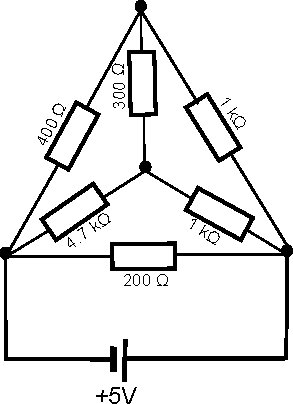
\includegraphics[scale=0.8]{ub.pdf}
		\caption{\"Ubungsbeispiel.}
	\end{center}
\end{figure}
\noindent
\section{Dynamische Stromkreise}
Bisher haben wir die Annahme getroffen, dass Strom und Spannung in einem elektrischen Netzwerk sich nicht mit der Zeit ver\"andert. Diese Annahme ist allerdings bis auf Netze, die sich nach dem Einschalten in einem konstanten Gleichgewichtzustand einfinden in physischen Netzwerken nie gegeben. Nach dem Einschalten eines elektrischen Ger\"ates braucht es immer eine gewisse Zeit bis die Spannung und der Strom von den Quellen zu den Bauteilen gelangt sind. Es gibt Anordnungen von elektrischen Bauteilen, die Schwingungen unterschiedlicher Formen erzeugen, sowie einen Effekt der bei Abschalten der Spannungsquelle beziehungsweise des Stromes dazu f\"uhrt, dass dieser nicht sofort wegf\"allt sondern langsam abklingt. All diese Effekte werden in diesem Abschnitt anhand von idealisierten Bauteilen erkl\"art. Abschlie\ss{}end werden Halbleiterbauteile wie Dioden und Feldeffekttransistoren behandelt, die uns dann erm\"oglichen im letzten Abschnitt dieses Kapitels die CMOS Technologie und darauf basierende logische Gatter zu verstehen.
\subsection{Der Kondensator}
 Ein Kondensator ist ein elektrisches Bauteil, dass Strom in eine dem Strom entgegengerichete Spannung umwandelt. Wir wollen in diesem Abschnitt nicht auf den Aufbau oder unterliegende physikalische Prinzip ein, sondern beschr\"anken uns auf eine Beschreibung basierend auf Strom und Spannung allein. Wer mehr wissen will kann \"uber die darunterliegende Physik im Anhang lesen oder in einem entsprecheden Fachbuch.
  \begin{figure}[H]
 	\begin{center}
 		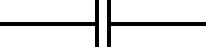
\includegraphics[scale=0.8]{kondens.pdf}
 		\caption{Schaltsymbol eines Kondensator.}
 	\end{center}
 \end{figure}
 \noindent
 Betrachten wir einen Schaltplan in dem ein Kondensator \"uber einen Widerstand und eine Gl\"uhbiren an eine Spannungsquelle geschlossen ist. 
 \begin{figure}[H]
 	\begin{center}
 		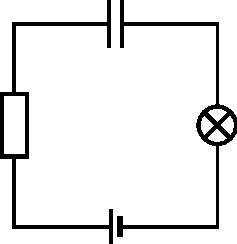
\includegraphics[scale=0.8]{kondensator.pdf}
 		\caption{Stromkreis mit Kondensator.}
 	\end{center}
 \end{figure}
 \noindent
 Eine m\"ogliche Realisierung dieses Schaltplanes w\"are eine Batterie die anuf einem Pol an einen Kondensator und am anderen Pol \"uber eine Gl\"uhbirne am anderen Pol des Kondensators geschlossen ist.\\
 Sobald wir den Stromkreis geschlossen haben wird entsprechend der Spannung an der Quelle, dem Widerstand der Leiter und der Gl\"uhbirne ein Strom im Uhrzeigersinn durch den Stromkreis flie\ss{}en. Der Kondensator wird diesen Strom in eine dem Strom und somit der Spannungsquelle (unten) entgegengerichtete Spannung umwandeln. Umso mehr Strom geflossen ist umso h\"oher wird diese umgekehrte Spannung und umso kleiner wird der Strom, da der Kondensator die an den Bauteilen anliegende Spannung verringert. Dies geht so lange bis der Kondensator betragsm\"assig dieselbe Spannung wie die Spannungsquelle hat und der Strom Null wird. Wir beobachten ensprechend beim Schlie\ss{}en des Stromkreises ein helles Aufleuchten der Gl\"uhbirne, das schnell dimmt und verschwindet.\\
 \\
 Entfernen wir nun die Spannungsquelle aus dem Stromkreis, und schlie\ss{}en den Kondensator direkt an die Gl\"uhbiren, sehen wir dasselbe Resultat. Die Gl\"uhbirne leuchtet auf, dimmt schnell und erlischt.\\
 \\
 Ein Kondensator speichert also Strom als Spannung, \"ahnlich wie eine aufladbare Batterie. Er hat daher einen Zustand, n\"amlich seine Spannung. \\
 Die Charakteristik eines Kondensators entspricht der einer idealen Spannungsquelle, deren Spannung von der Summe, der durch Str\"ome, zugeflossenen elektrischen Ladung abh\"angt. Hierbei tragen Str\"ome in eine Richtung als positiver Beitrag und Str\"ome in die andere Richtung als negativer Beitrag zur Summe bei.\\
 Wir werden daher jedem Kondensator, genauso wie einer Kante, eine Vorzugsrichtung zuordnen. Die Charakteristik soll einer idealen Spannungsquelle mit Plus Pol in Vorzugsrichtung entsprechen.
  \begin{figure}[H]
 	\begin{center}
 		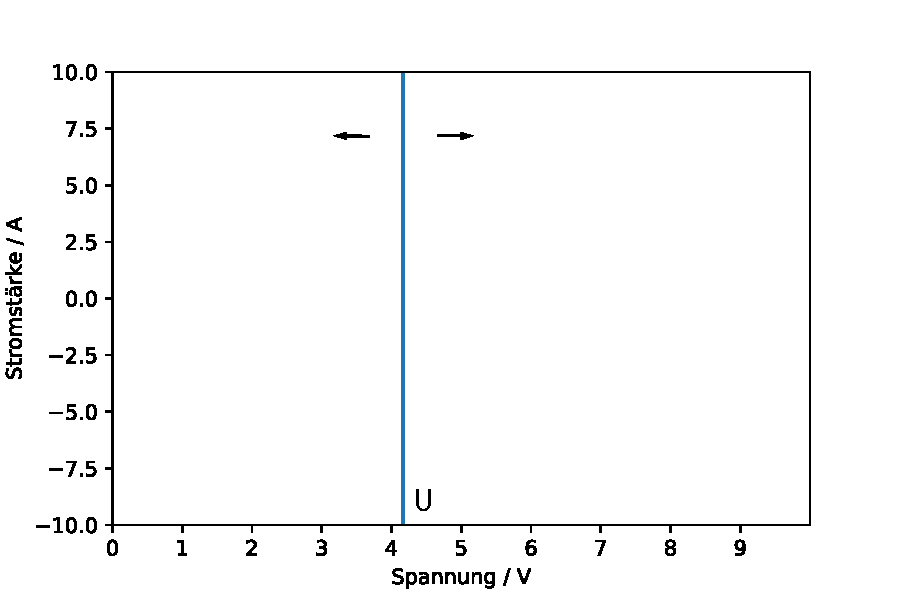
\includegraphics[scale=0.5]{variable_Spannungsquelle.pdf}
 		\caption{Charakteristik variable Spannungsquelle}
 	\end{center}
 \end{figure}
 \noindent
Jedem Kondensator in einem elektrischen Netz wird ein Zustand, seine Spannung $U$ zugeordnet. Um diese Spannung zu interpretieren m\"ussen eine Vorzugsrichtung und anliegende Potentiale gegeben sein
  \begin{figure}[H]
	\begin{center}
		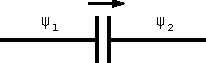
\includegraphics[scale=1]{kkondens.pdf}
	\end{center}
\end{figure}
\noindent
Wir schreiben nun, unter Beachtung der Vorzugsrichtung.
\begin{equation*}
	\psi_2 - \psi_1 = U
\end{equation*}
Dies entspricht genau der Gleichung, die wir f\"ur eine ideale Spannungsquelle mit Pluspol in Vorzugsrichtung erhalten w\"urden.
Es wird ein linearer Zusammenhang zwischen dem Differentialquotienten der Spannung $U$ nach der Zeit $t$ und dem Strom $j$ angenommen. 
 \begin{equation}
 	\frac{dU}{dt} = -\frac{j}{c} 
 \end{equation}
 \noindent
 Das negative Vorzeichen ber\"ucksichtigt, dass die durch den Strom aufgebaute Spannung im Kondensator immer gegen den Strom wirkt.Die Konstante $c$ nennt man auch die Kapazit\"at des Konsensators. Sie gibt an wie viel elektrische Ladung $q$ zuflie\ss{}en muss um eine gegebene den Strom antreibende Spannung zu erreichen.
  \begin{equation}
	c = \frac{q}{U} 
  \end{equation}
 \noindent
 Als Konsequenz von (4.18) wird das zu einem Schaltplan geh\"orende Gleichungssystem zu einem Differentialgleichungssystem. Also zu einem System von Gleichungen, dass nicht einen Satz von reelen Zahlenwerten f\"ur jede Potentialvariable festlegt, sondern Funktionen, die jedem Zeitpunkt einen reelen Zahlenwert zuordnet.\\
 \\
 Wir werden im Rest dieses Abschnittes das in Worten beschriebene Experiment zu Abbildung (4.22) nachrechnen. Hierzu vereinfachen wir den Stromkreis indem wir die Gl\"uhbirne und den Widerstand zu einem einzigen Widerstand verschmelzen. Dies f\"uhrt zum selben Ergebnis, wenn wir annehmen, dass die Gl\"uhbirne eine lineare Charakteristik hat und der resultierende Widerstand nach der Reihenschaltungsformel(4.9) berechnet wird.
   \begin{figure}[H]
 	\begin{center}
 		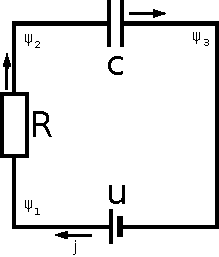
\includegraphics[scale=1]{einfach.pdf}
 	\end{center}
 \end{figure}
 \noindent
 In der Abbildung wurden bereits alle Vorzugsrichtungen, Potentiale und Str\"ome, sowie Paramter $c$, $R$ und $u$ eingezeichnet. Als Gleichungssystem ausformuliert bedeutet dies.
 \begin{align} 
 	\psi_1 = \psi_3 + u\\
	j = \frac{\psi_1 - \psi_2}{R}\\
	\frac{d(\psi_3 - \psi_2)}{dt} = - \frac{j}{c}
 \end{align}
Wir werden wie gehabt annehmen, dass $\psi_3 = 0$, wodurch $\psi_1 = u$ ist und wir das Problem auf eine Unbekannte, n\"amlich $\psi_2$ reduziert haben.
\begin{equation}
	\frac{d\psi_2}{dt} = \frac{u - \psi_2}{R c}
\end{equation}
Dies ist eine inhomogene lineare Differentialgleichung, die beschreibt wie sich das Potential $\psi_2$ mit der Zeit entwickelt. Es fehlt uns nur noch ein Startwert f\"ur die Spannung am Kondensator $U$ und wir k\"onnen eine eindeutige L\"oesung aufschreiben. \\
\\
Dies f\"uhrt uns zu den Szenarien unterhalb von Abbildung (4.22). Starten wir mit dem Szenario wo wir eine Spannungsquelle an einen Kondensator schlie\ss{}en. Der Kondensator ist zu Beginn ungeladen also $U(0) = 0$.
Dies f\"uhrt zur eindeutigen L\"osung:
\begin{equation}
	\psi_2(t) = u * (1 - e^{-\frac{t}{Rc}})
\end{equation}
Setzen wir den Widerstand $R$ gleich $10k\Omega$, die Spannung $u$ auf $5V$ und die Kapazit\"at $c$ gleich $10nAs/V$ und betrachten die Kurve.
   \begin{figure}[H]
	\begin{center}
		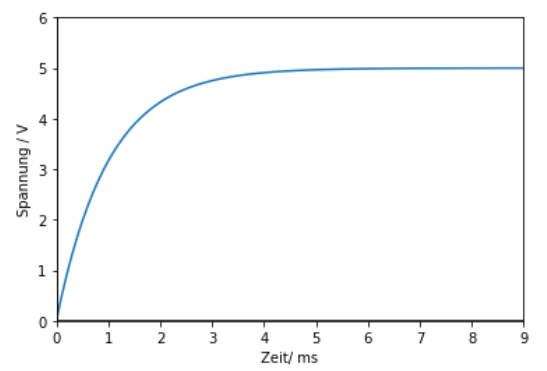
\includegraphics[scale=0.5]{Ladung.png}
	\end{center}
\end{figure}
\noindent
Zu Beginn steigt die Spannung sehr rasch an und es stellt sich schnell ein Gleichgewicht mit der Spannungsquelle ein wodurch nur mehr ein kleiner werdender schwacher Strom flie\ss{}t.\\
\\
Im zweiten Szenario nehmen wir an, dass wir den nun geladenen Kondensator von der Spannungsquelle nehmen und direkt an den Widerstand schlie\ss{}en. Hierzu setzen wir $u$ einfach Null, was die Spannungsquelle aus dem Stromkreis eliminiert und setzen die Spannung des Kondensators $U$ gleich $5V$.
\begin{equation}
\psi_2(t) = 5 * e^{-\frac{t}{Rc}}
\end{equation}
Wir setzen die Paramter $c$ und $R$ wie gehabt und erhalten, einen exponentiellen Abfall der Spannung.
   \begin{figure}[H]
	\begin{center}
		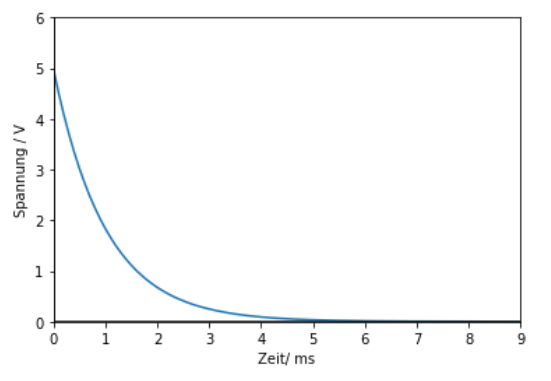
\includegraphics[scale=0.5]{entladung.png}
	\end{center}
\end{figure}
\noindent
Wie im ersten Szenario folgt auf eine schnelle \"Anderung der Spannung eine Abflachung und S\"attigung. Der Strom verh\"alt sich entsprechend dem Ohmschen Gesetz hier analog zur Spannungskurve. \\
\\
Damit haben wir die Ladesituation sowie die Entladungssituation eines Kondensators im Detail beschrieben und nachgerechnet. \\
\\
In einem physikalsichen elektrischen Netzwerk verhalten sich so gut wie alle elektrischen Bauteile und somit auch die Kabelverbindungen zwischen Diesen wie ein Kondensator mit sehr kleiner Kapazit\"at. Dies f\"allt kaum auf solange im Netzwerk keine all zu hoch frequenten Prozesse stattfinden. Kann aber zum Problem werden, wenn zum Beispiel unsere Rechenmaschine eine sehr hohe Taktfrequenz hat. Man spricht hier von kapazitiven Effekten und wenn wir sie ber\"ucksichtigt wollen, dann kann dies einfach gemacht werden indem man einen Kondensator in parallel mit dem ensprechenden Bauteil im Schaltplan zeichnet. Wenn zwei Bauteile kapazitiv wechselwirken, also sich zusammen wie ein Kondensator verhalten, dann verbinden wir sie \"uber einen Kondensator mit der entsprechenden Kapazit\"at.
\subsection{Die Spule}
Eine Spule ist ein zweipoliges elektrisches Bauteil, dass sich einer \"Anderung des elektrischen Stromes durch eine, der \"Anderung entgegen gerichtete, Spannung widersetzt. Man sagt die Strom\"anderung induziert eine Spannung in der Spule. Das zugrunde liegende physikalsiche Prinzip nennt man Induktion beziehungsweise Selbstinduktion und wird im Anhang n\"aher erkl\"art.
Wir wollen aber hier, wie bereits beim Kondensator, das Bauteil anhand der f\"ur uns interessanten Ph\"anomene Spannung und Stromst\"arke beschreiben.
  \begin{figure}[H]
	\begin{center}
		
\includegraphics[scale=1.5]{spule.pdf}
		\caption{Schaltsymbol einer Spule.}
	\end{center}
\end{figure}
\noindent
Starten wir wieder mit einem einfachen Experiment. Wir nehmen eine Spule und verbinden sie an einer Seite mit einer Gl\"uhbirne und schlie\"ss{}en dies in parallel mit einer weiteren Gl\"uhbirne an eine Spannungsquelle. 
Der beschriebene Sachverhalt entspricht dem in Abbildung (4.25) dargestellten Schaltpan.
  \begin{figure}[H]
	\begin{center}
		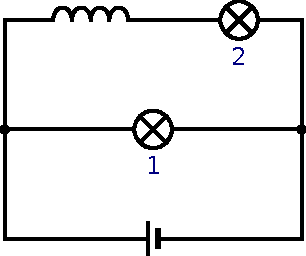
\includegraphics[scale=1]{spulensg.pdf}
		\caption{Experiment zu Induktion.}
	\end{center}
\end{figure}
\noindent
Wenn eine stark genuge Spule\footnote{Was das hei\ss{} sehen wir im Laufe dieses Abschnittes.} gew\"ahlt wurde, sehen wir beim schlie\ss{} der Spannungsquelle an den Stromkreis Lampe Nummer eins sofort aufleuchten, aber Lampe Nummer zwei leuchtet anfangs nur gedimmt und erreicht seine volle Leuchtst\"arke erst einen Moment sp\"ater.
Unterbrechen wir nun den Stromkreis indem wir die Spannungsquelle entfernen, beobachten wir, dass Lampe eins und zwei noch einen Moment nachleuchten.\\
\\
Im Gegensatz zum Kondensator speichert eine Spule also anscheinend elektrischen Strom. Zuerst will sie ihn bei Null lassen und nachdem er seinen S\"attungsstrom nach dem Ohmschen Gesetz erreicht hat, versucht es diesen beizubehalten, auch nachdem die treibende Spannung genommen wurde.
\\
\\
Woher kommt aber dieser Strom, nachdem die Spannungsquelle entnommen wurde? Es gelten ja noch immer die Grundgesetze elektrischer Netzwerke, also muss der Strom von einer Spannung begleitet werden. Diese Spannung nennt man induzierte Spannung und sie ist immer der Richtung der \"Anderung des Stromes entgegengerichtet. Wenn wir also beim Entfernen des Stromkreises die an der Spule anliegende Spannung gemessen h\"atten, so w\"are sie der Richtung der gerade entfernten Spannungsquelle entegegengesetzt gewesen.\\
\\
Analog zum Kondensator nehmen wir an, dass die Spule die Charakteristik einer idealen Spannungsquelle (4.23) mit ver\"anderlicher Spannung $U$ hat. Die Spule hat ebenfalls wie der Kondensator eine Zustand und zwar die durch sie flie\ss{}ende Stromst\"arke.
Entsprechend wird einer Spule eine Vorzugsrichtung gegeben wie einer Kante und es gilt wie beim Kondensator.
  \begin{figure}[H]
	\begin{center}
		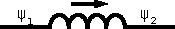
\includegraphics[scale=1.5]{spule_direkt.pdf}
	\end{center}
\end{figure}
\noindent
Da wir die Spule wie eine ideale Spannungsquelle behandeln gilt wieder.
\begin{equation*}
\psi_2 - \psi_1 = U
\end{equation*}
Die induzierte Spannung $U$ h\"angt linear vom Differentialquotienten der Stromst\"arke $j$ nach der Zeit $t$ ab.
 \begin{equation}
\frac{dj}{dt} = -\frac{U}{L} 
\end{equation}
\noindent
Vergleiche Gleichung (4.26) mit (4.18) und erkenne, dass sich Kondensator und Spule analog verhalten, wobei die Rolle von Strom und Spannung vertauscht ist.\\
\\
Die Konstante $L$ nennen wir die Induktivit\"at der Spule und sie wird in $Vs/A$ gemessen. Genauso wie beim Fall des Kondensators erhalten wir bei einer Spule ein Differentialgleichungssystem, dass einen Satz von Funktionen f\"ur jeden Potentialwert bestimmt.\\
\\
Kommen wir nun zur\"uck zum Experiment zu Abbildung (4.25) zur\"uck und rechnen dieses mit Hilfe der nun bekannten Gesetzm\"assigkeiten nach. Der Schaltplan wird hierzu wieder vereinfacht indem jede Gl\"uhbirne durch einen ohmschen Widerstand ersetzt wird.
  \begin{figure}[H]
	\begin{center}
		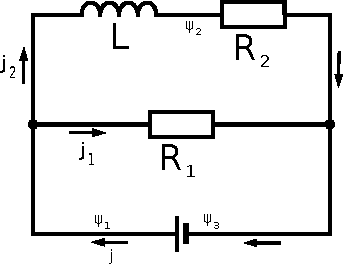
\includegraphics[scale=1]{spuledir.pdf}
	\end{center}
\end{figure}
\noindent
In der Abbildung sind bereits alle Vorzugsrichtungen, Potentiale und Parameter eingezeichnet. Es verbleibt nur noch das resultierende Gleichungssystem aufzuschreiben.\\
\\
Zuerst die Bauteilgleichungen:
 \begin{align} 
\psi_1 = \psi_3 + u\\
j_1 = \frac{\psi_1 - \psi_3}{R_1}\\
j_2 = \frac{\psi_2 - \psi_3}{R_2}\\
\frac{dj_2}{dt} = -\frac{\psi_2 - \psi_1}{L}
\end{align}
und dann die Knotenregel:
\begin{equation*}
	j = j_1 + j_2
\end{equation*}
Wir setzen wieder $\psi_3=0$, woraus $\psi_1=u$ folgt und erhalten durch Umformung:
 \begin{align} 
\frac{d\psi_2}{dt} = -\frac{R_2}{L} (\psi_2 - u)
\end{align}
Dies entspricht der Differentialgleichung (4.23), die wir bei unserer Diskussion des Kondensators kennen gelernt haben. Der Anfangszustand unseres Stromkreises ist $j_2(0) = 0$. Wir haben aber unseren Stromkreis \"uber das Potential $\psi_2$ beschrieben.  Daher m\"ussen wir unsere Anfangsbedingung \"uber (4.29)  umwandeln in eine die $\psi_2$ betrifft und zwar $\psi_2(0) = \psi_3(0) = 0$.\\
\\
Unser erstes Experiment entspricht also bis auf die Konstanten genau dem ersten Experiment, dass wir beim Kondensator kennen gelernt haben. Wir k\"onnen daher die L\"oesung (4.24) kopieren.
\begin{equation}
\psi_2(t) = u * (1 - e^{-\frac{R_2 t}{L}})
\end{equation}  
Nehmen wir wie beim Kondensator ein konkretes Beispiel heran. Die Spule hat eine Induktivit\"at $L=0.1 Vs/A$, $R_1=100\Omega$ und $R_2=100\Omega$ und die Spannungsquelle eine Spannung $u=5V$.
\begin{figure}[H]
	\begin{center}
		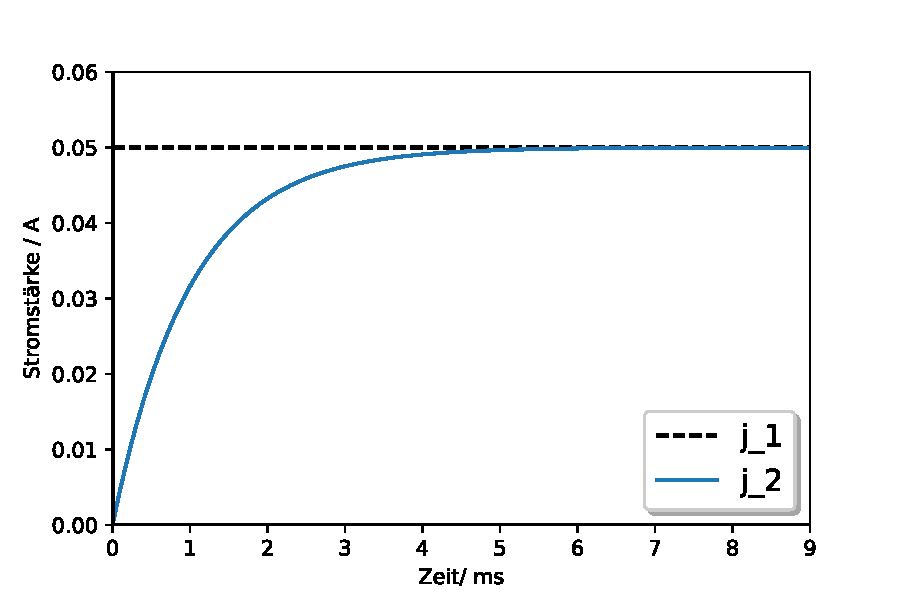
\includegraphics[scale=0.75]{spule_j.pdf}
		\caption{Stromst\"arken zu Experiment 1.}
	\end{center}
\end{figure}
\noindent
Die Abbildung zeigt die Stromst\"arken der Gl\"uhbirne 1 und 2. Es zeigt sich ganz analog zu unserem Experiment, dass der Strom durch Gl\"uhbirne 2 etwas l\"anger braucht um seine volle St\"arke zu erreichen. Dies entspricht einem Ladevorgang der Spule.\\
\\
Kommen wir nun zum zweiten Experiment, wo wir von dem Stromkreis (4.25), nachdem beide Gl\"uhbirnen konstant leuchten, die Spannungsquelle aus dem Stromkreis entfernen. Hierzu m\"ussen wir etwas an unseren Variablen \"andern und erhalten folgenden Schaltplan, der den Sachverhalt nach der Entfernung widerspiegelt.
  \begin{figure}[H]
	\begin{center}
		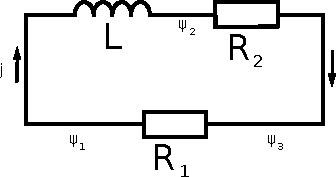
\includegraphics[scale=1]{spuledir2.pdf}
	\end{center}
\end{figure}
\noindent
Im Abschnitt \"uber Reihenschaltung haben wir gesehen, dass sich dies vereinfachen l\"asst, sei hierzu $R = R_1 + R_2$.
  \begin{figure}[H]
	\begin{center}
		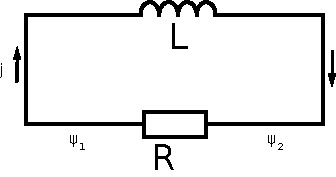
\includegraphics[scale=1]{spuledir3.pdf}
	\end{center}
\end{figure}
\noindent
Wir haben damit beide Gl\"uhbirnen zu einem Bauteil vereinigt und erhalten folgendes Gleichungssytem, wobei wir $\psi_2$ schon Null gesetzt haben:
 \begin{align} 
j = \frac{\psi_1}{R}\\
\frac{dj}{dt} = \frac{\psi_1}{L}
\end{align}
Durch Einsetzen erhalten wir die Differentialgleichung,
\begin{equation}
\frac{d\psi_1}{dt} = \frac{R}{L}\psi_1
\end{equation}  
die unter der Annahme, dass $j(0) = u/R$ und somit $\psi_1(0)=u$ zur L\"osung
\begin{equation*}
\psi_1(t) = u * e^{-\frac{R t}{L}})
\end{equation*}  
f\"uhrt.\\
\\
Betrachten wir abschlie\ss{}end noch den Verlauf von $j$ in diesem Experiment.
  \begin{figure}[H]
	\begin{center}
		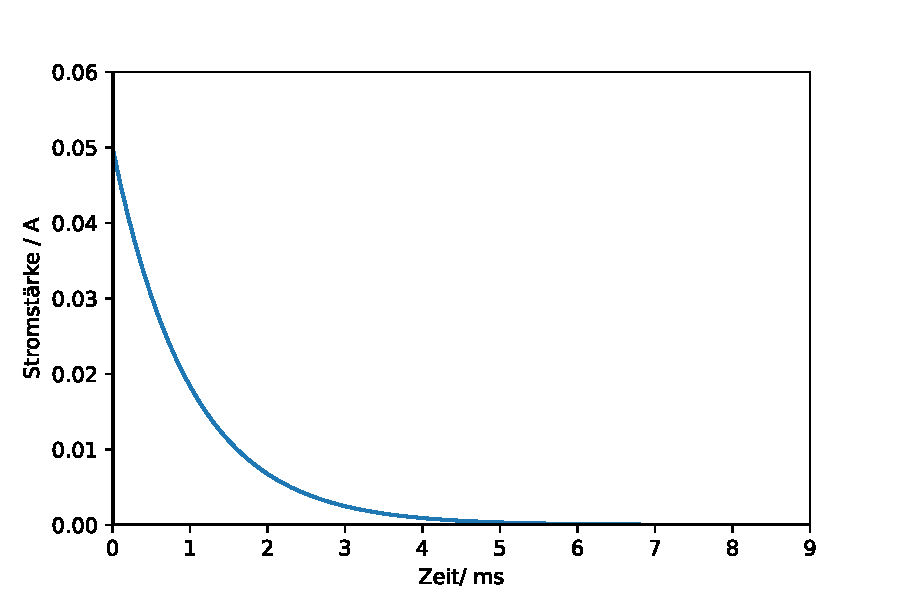
\includegraphics[scale=0.75]{entladungsspule.pdf}
	\end{center}
\end{figure}
\noindent
Genauso wie beim ersten Experiment, sehen wir auch beim zweiten Experiment ein analoges Verhalten zum zweiten Experiment im Kondensator Abschnitt.\\
Die Stromkurve f\"allt zun\"achst rasch und stellt sich dann langsam gegen Null ein. Dies entspricht genau dem Verhalten, dass wir beim Experiment beschrieben haben, denn bei $t=0$ wird hier die Spannungsquelle entfernt und die Spule die mit einer Stromst\"arke von $u/R_2$ geladen war, entl\"dt sich.\\
\\
Zum Abschluss soll noch einmal auf die Analogie zwischen Spule und Kondensator hingewiesen werden. Man kann sich Experiment eins und zwei jeweils als Ladevorgang und Entladevorgang der Spule denken. Es wurden beide beschrieben und nachgerechnet.\\
\\
Die Analogie zieht sich aber noch weiter, denn genauso wie sich in einem physikalischen elektrischen Netzwerk jedes Bauteil sowie auch die Kabel- verbindungen wie ein Kondensator mit schwacher Kapazit\"at verhalten, verhalten sie sich auch wie eine Spule mit schwacher Induktivit\"at.\\
Entsprechend muss man auch so genannte induktive Effekte ber\"ucksichtigen, wenn man ein elektrisches Netzwerk plant. Ein bekannter Effekt der Induktvit\"at ist der Funken\"uberschlag beim \"offnen eines Schalters oder die zeitliche Verz\"ogerung bei sehr langen Netzwerken.\\
Will man das induktive Verhalten eines elektrischen Bauteiles im Schaltplan ber\"ucksichtigen, wird eine Spule mit entsprechender Induktivit\"at vor oder nach dem Bauteil in Reihe geschaltet. Es gibt noch induktive Effekte die \"uber die hier besprochenen Effekte hinausgehen. Hierzu geh\"oren allgemeine elektromagnetische Effekte, die im Anhang besprochen werden.
\subsection{Der Schwingkreis}
In den letzten beiden Abschnitten haben wir einen Speicher f\"ur Strom, die Spule und einen Speicher f\"ur Spannung, den Kondensator kennen gelernt. Nun ist es so, dass ein Kondensator durch einen Strom geladen wird, und sich \"uber einen Strom entl\"adt. Auf der anderen Seite ist es so, dass eine Spule \"uber eine Spannung geladen wird und sich \"uber eine Spannung entl\"adt.\\
\\
Es ist daher leicht zu sehen, dass wenn wir eine Spule und einen Kondensator kombinieren in einer Schleife, die eine Komponente die andere Komponente beim entladen aufl\"adt und umgekehrt. Dies f\"uhrt zu einem zyklischen oder periodischen Verhalten des Stromkreises. \\
In diesem Abschnitt werden wir uns entwas n\"aher mit diesem Ph\"anomen auseinandersetzen und nachrechnen was genau passiert und wie ein ohmscher Widerstand das Verhalten beeinflu\ss{}t.\\
\\
Betrachten wir zun\"achst den einfacheren Fall, den so genannten unged\"ampften Schwingkreis, n\"amlich eines Kondensators, der direkt an eine Spule geschlossen wird. Nehmen wir an, dass der Kondensator anfangs geladen ist und kein Strom flie\ss{}t und berechnen wie sich der Strom und die Spannung mit der Zeit entwickelt.
\begin{figure}[H]
	\begin{center}
		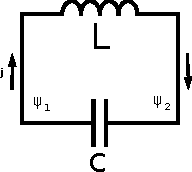
\includegraphics[scale=1]{schnwingkreis_ungedampft.pdf}
		\caption{Unged\"ampfter Schwingkreis.}
	\end{center}
\end{figure}
\noindent
Wir nehmen wieder an, dass $\psi_2=0$ und k\"onnen sofort die Differentialgleichungen aufschreiben.
 \begin{align} 
\frac{dj}{dt} = \frac{\psi_1}{L}\\
\frac{d\psi_1}{dt} = -\frac{j}{c}
\end{align}
Durch Einsetzen von (4.37) in (4.36) erhalten wir die Gleichung:
\begin{equation}
	\frac{d^2\psi_1}{dt^2} = -\frac{\psi_1}{Lc}
\end{equation}
Diese Gleichung ist bekannt als der klassische harmonische Oszillator und besitzt die allgemeine L\"osung:
\begin{equation}
	\psi_1(t) = a \cos(\frac{t}{Lc}) + b \sin(\frac{t}{Lc})
\end{equation}
Wir haben also zwei Unbekannte, die durch die Anfangsbedingung bestimmt werden sollen. Die Anfangsbdingung lautet $\psi_1(0) = u$ und $j(0) = 0$. Betrachten wir zun\"achst die allemeine L\"osung und ihre Ableitung zum Zeitpunkt $t=0$.
 \begin{align} 
\psi_1(0) = a \cos(\frac{0}{Lc}) + b \sin(\frac{0}{Lc}) = a\\
\frac{d\psi_1}{dt}(0) = -\frac{a}{Lc} \sin(\frac{0}{Lc}) + \frac{b}{Lc} \cos(\frac{0}{Lc}) = \frac{b}{Lc}
\end{align}
Aus GLeichung (4.37) und $j(0) = 0$ folgt zusammen mit (4.41), dass $b=0$ und aus der Anfangsbedingung $\psi_1(0) = u$ k\"onnen wir mit (4.40) schlie\ss{}en, dass $a=u$. Die L\"osung unseres Problems lautet also:
\begin{equation}
	\psi_1(t) = u * \cos(\frac{t}{Lc})
\end{equation}
In graphischer Form dargestellt sieht das bei einem Kondensator mit Kapazit\"at $c=1nF$ und einer Spule mit Induktivit\"at $L=1H$ folgenderma\ss{}en aus.
  \begin{figure}[H]
	\begin{center}
		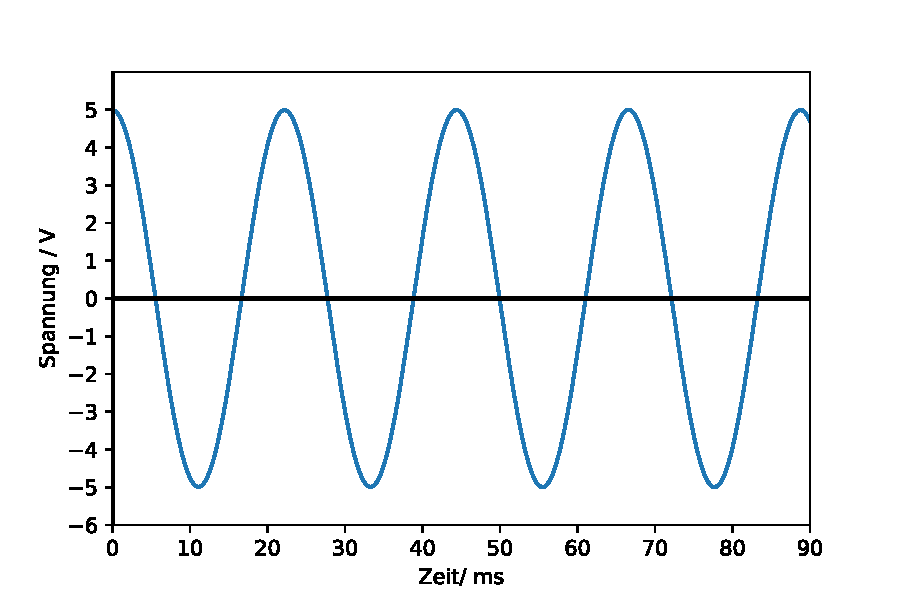
\includegraphics[scale=0.75]{harmonisch.pdf}
	\end{center}
\end{figure}
\noindent
Man sieht ein periodisches Verhalten des Spannungssignals, was analog auch f\"ur den Strom gilt. Dieser periodische Vorgang w\"urde sich unendlich fortsetzen wenn man ihn lie\ss{}e. In der Praxis ist eine derartige Schaltung aber unm\"oglich, da der Kondensator und die Spule nur Idealisierungen darstellen.\\
Vor allem ist in einem echten Schaltkreis auch immer die Charakteristik der verbindenden Dr\"ahte, also ein ohmscher Widerstand, beteiligt.\\
\\
Warum nennen wir diese Schaltung einen \textbf{ged\"ampften} Schwingkreis? Um diese Frage zu beantworten betrachten wir die Energie, die ein Kondensator bei einer bestimmten Spannung $U$ h\"alt. 
\begin{equation}
	E_c(U) = \frac{1}{2}c * U^2
\end{equation}
Die Energie erh\"alt man durch Integration der Leistung nach der Zeit. In diesem Fall verwendeten wir Gleichung (4.18) und die Formel f\"ur die elektrische Leistung (4.1).\\
Analog errechnet sich die Energie die bei einer bestimmten Stromst\"arke $I$ in einer Spule gespeichert ist aus (4.26) und erh\"alt.
\begin{equation}
	E_L(I) = \frac{1}{2}L * I^2
\end{equation}
Wir k\"onnen $E_L$ als die kinetische Energie und $E_c$ als die potentielle Energie in Analogie zur Mechanik. Die Gesamtenergie eines geschlossenen Systems bleibt erhalten und da wir Verluste durch W\"arme und elektromagnetischen Wechselwirkung mit der Umgebung vernachl\"assigt wurde, gilt dies auch hier. Also wenn wir die L\"osung (4.42) und den sich daraus ergebenden Strom nach (4.37) einsetzen erhalten wir.
\begin{align*}
E_{ges}(\psi_1) = E_L(-c\frac{d\psi_1}{dt}) + E_c(\psi_1)\\
= \frac{1}{2}(Lc^2(\frac{d\psi_1}{dt})^2  + c(\psi_1)^2) = \frac{1}{2}cu^2
\end{align*}
Dies zeigt, dass die Gesamtenergie $E_{ges}$ konstant bleibt f\"ur alle Zeiten und zwar mit dem Startwert der Energie des geladenen Kondensators.\\
\\
D\"ampfung ist ein Resultat von Termen in der dynamischen Gleichung, die Energie an die Umgebung abf\"uren. Ein Ohmscher Widerstand gibt uns einen solchen Term. Er wandelt elektrische Energie bei Stromdurchfluss in W\"arme um, die so genannte Joulesche W\"arme.\\
\\
Widmen wir uns um n\"aher an die Realit\"at zu kommen, kurz dem ged\"ampften Schwingkreis in dem einfach zus\"atzlich ein Widerstand zwischen Kondensator und Spule geschaltet ist.
  \begin{figure}[H]
	\begin{center}
		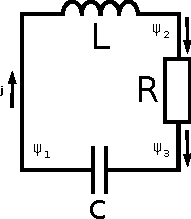
\includegraphics[scale=1]{schnwingkreis_gedampft.pdf}
	\end{center}
\end{figure}
\noindent
Wir setzen wieder $\psi_3=0$ und lesen direkt das zugeh\"orige Differentialgleichungssystem ab.
\begin{align}
	\frac{dj}{dt} = -\frac{\psi_1 - j*R}{L}\\
	\frac{d\psi_1}{dt} = -\frac{j}{c}
\end{align}
Durch Einsetzen von (4.45) in (4,46) erhalten wir wieder eine Differentialgleichung mit einer zweiten Ableitung.
\begin{equation}
	\frac{d^2\psi_1}{dt^2} + \frac{R}{L}\frac{d\psi_1}{dt} + \frac{1}{Lc}\psi_1 = 0
\end{equation}
Dies ist eine lineare Differentialgleichung mit konstanten Koeffizienten, genauso wie der harmonische Oszillator, nur eben mit einem D\"ampfungsterm. Eine solche Gleichung l\"asst sich mit einem Exponentialansatz l\"osen. Setzen wir hierzu eine Funktion $\psi_1$ der Form
\begin{equation}
\psi_1(t) = a*e^{\lambda*t}
\end{equation}
in die Gleichung (4.47) ein wobei $\lambda$ eine unbekannte komplexe Zahl ist. 
Exponentialfunktionen sind immer positiv also k\"onnen wir nach Einsetzen auf eine quadratische Gleichung reduzieren.
\begin{equation}
\lambda^2 + \frac{R}{L}\lambda + \frac{1}{Lc} = 0
\end{equation}
Es gibt entweder zwei komplexe Zahlen $\lambda_1$ und $\lambda_2$, oder nur eine komplexe Zahl $\lambda$, die diese Gleichung aufl\"ost. 
\paragraph{\"Ubungsbeispiel:} Verwende die L\"osungsformel f\"ur quadratische Gleichungen um die Gleichung (4.49) zu l\"osen.\\
\\
Wir k\"onnen direkt an der L\"osungsformel ablesen, dass wir bis auf einen Grenzfall und zwar wenn $R^2*c = 4*L$ gilt, zwei L\"osungen erwarten.
Heben wir uns den Grenzfall erstmal auf und behandeln den Fall mit zwei L\"osungen. Unser Anfangswertproblem zu (4.47) verlangt zwei unabh\"angige L\"osungsfunktionen, da wir zwei Anfangsbedingungen haben, $j(0)=0$ und $\psi_1(0) = u$. \\
Setzen wir nun f\"ur $\psi_1$ in (4.47) 
\begin{equation}
\psi_1(t) = a*e^{\lambda_1*t} + b*e^{\lambda_2*t}
\end{equation}
und suchen Werte f\"ur die Unbekannten $a$ und $b$, sodass die Anfangsbedingung erf\"ullt sind. 
Wir gehen hier genauso vor wie beim unged\"ampften Fall und erhalten die L\"osung.
\begin{equation}
\psi_1(t) = \frac{\lambda_2*u}{\lambda_2 - \lambda_1}*e^{\lambda_1*t} + \frac{\lambda_1*u}{\lambda_2 - \lambda_1}*e^{\lambda_2*t}
\end{equation}
\paragraph{\"Ubungsbeispiel:} Führe die Berechnung durch, die zu gegebenen Anfangswerten $j(0)$ und $\psi_1(0)$ Werte f\"ur $a$ und $b$ liefert.\\
\\
Betrachten wir die graphische Darstellung des zeitlichen Verlaufes der Spannungskurve mit den selben Werten f\"ur Induktivit\"at und Kapazit\"at wie in der vorherigen Darstellung im unged\"ampften Fall, f\"ur drei Werte des Widerstandes $R$.
\begin{figure}[H]
	\begin{center}
		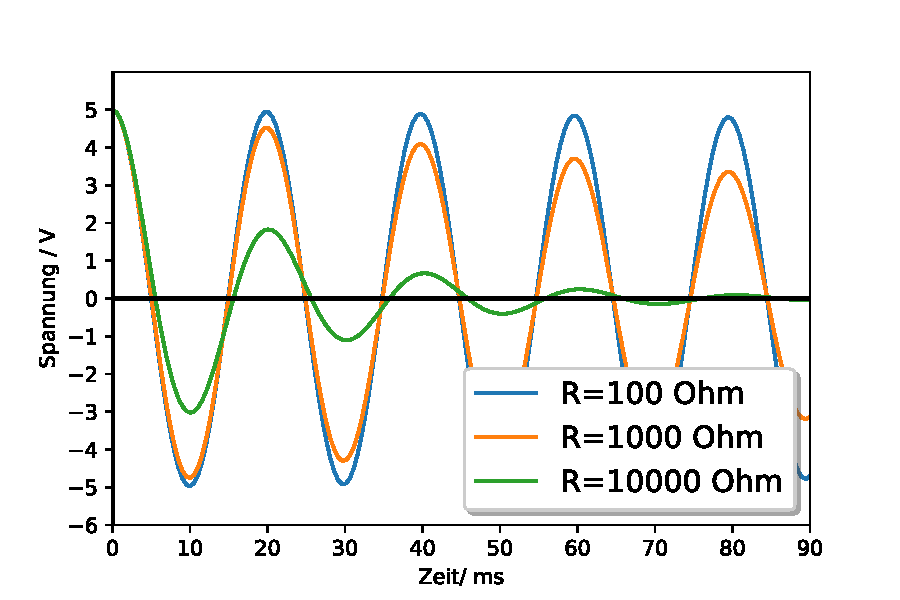
\includegraphics[scale=0.75]{dampf.pdf}
	\end{center}
\end{figure}
\noindent
Wir sehen, dass eine D\"ampfung stattfindet, daher die vormals periodische Funktion mit der Zeit abklingt. Dieses Abklingen ist umso schneller, desto gr\"o\ss{}er der elektrische Widerstand im Schwingkreis ist.\\
\\
Wenn wir das Ganze von der Perspektive der Energie im Schwingkreis aus betrachten, verh\"alt sich der Widerstand wie ein Leck, das mit der Zeit Energie an die Umwelt abgibt. Diese Jouleschen Verluste sind f\"ur den D\"ampfungseffekt verantwortlich.
\\
\\
Im Fall wenn es nur eine L\"osung der Gleichung (4.50) gibt, in der Literatur als aperiodischer Grenzfall bezeichnet,  m\"ussen wir den Ansatz 
\begin{equation}
	\psi_1(t) = a*e^{\lambda*t} + b*t*e^{\lambda*t}
\end{equation}verwenden. 
\paragraph{\"Ubungsbeispiel:} Finde die L\"osung im aperiodischen Grenzfall.\\
\\
Das Thema Schwingkreis lie\ss{}e sich noch wesentlich detailierter darstellen. Der ged\"ampfte Schwingkreis ist immer noch eine Idealisierung und wir sind nicht auf ein \"au\ss{}eres Spannungssignal eingegangen, dass wom\"oglich den Schwingkreis treibt. 
\subsection{Die Diode}
Eine Diode ist ein zweipoliges nichtlineares elektrisches Bauteil, dass Strom in eine Richtung sehr gut und in die entgegengesetzte Richtung bei moderat niedrigen Spannungen kaum leitet. Es gibt sehr viele verschiedene Bauformen und Implementierungen in verschiedenen Substraten. An sich ist eine Diode kein dynamisches Bauteil, aber Implementierungsabh\"angig kann es eine zeitliche Charakteristik haben und unabh\"angig von der Implementierung ist sie in Sperrrichtung immer auch ein Kondensator.
\begin{figure}[H]
	\begin{center}
		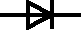
\includegraphics[scale=1.5]{diode.pdf}
		\caption{Schaltsymbol einer Diode.}
	\end{center}
\end{figure}
\noindent
Am Schaltsymbol einer Diode sehen wir sofort, dass es sich um ein Bauteil mit asymmetrischer Charakteristik handelt. Der Pfeil gibt hierbei die bevorzugte Stromrichtung an und die vertikale Linie ist auf der Seite aus welcher der Strom nicht kommen darf.\\
\\
\subsection{Der Feldeffekt Transitor}




\chapter{Ein m\"oglichst einfacher Digitalrechner}
Ein Digitalrechner hat zwei Buchstaben, n\"amlich die Null und die Eins, aber zus\"atzlich hat jeder eine meistens fixe Wortgr\"o\ss{}e, die in der Anzahl der Stellen , der Bits beziehungsweise Buchstaben, also der Nullen und der Einsen, welche die Maschine als ein Wort betrachtet, gemessen wird. Dieses Wort ist das eigentliche Elementare Objekt der Rechenmaschine, jede Operation wird nicht auf einem einzelnen Bit, also auf einer Stelle des Wortes, sondern immer auf dem gesamten Wort ausgef\"uhrt. Genauso holen wir wenn wir den Inhalt einer Speicheraddresse zum Rechenkern holen immer ein ganzes Wort, dass dort steht und nicht einen einzelnen Bit.
Ein Wort kann dabei f\"ur einen Buchstaben stehen, f\"ur eine Zahl oder die Addresse eines anderen Wortes. 
\section{Eine minimale Arithmetisch logische Einheit}
Die Idee einer digitalen Rechenmaschine mit der kleinst m\"oglichen Anzahl an arithmetischen und logischen Operationen, die in Kombination eine universelle Rechenmaschine ergeben, hat mich fasziniert, seit ich mir Gedanken \"uber den Bau von Rechenmaschinen gemacht habe. Solche Minimal Konstruktionen sind in der Regel nur
in der Theorie interessant, da sie nat\"urlich mehr Rechenschritte ben\"otigen als Maschinen mit mehreren Rechenoperationen. Diese zus\"atzlichen Rechenoperationen sind, zwar redundant was f\"ur bestimmte Menschen ein Sch\"onheitsfehler sein kann, aber Schnelligkeit und praktikabilit\"at sind in der echten Welt wichtiger.\\
\\
Meine arithmetisch logische Einheit hat die folgenden zwei Operationen:
\paragraph{NAND: } Die verneinte-Und Operation, die wie wahrscheinlich wie jedem Leser bekannt, durch verschiedene Kombinationen mit sich selbst, jede erdenkliche boolsche Operation erzeugen kann. Somit lassen sich s\"amtliche logischen Funktionen mit dieser Operation ausdr\"ucken. Zus\"atzlich setzt die NAND-Operation falls das NULL-Wort als Ergebnis erhalten wird ein Flag.
\paragraph{LSHIFT:} Der links shift beziehungsweise die Linksverschiebung, bei der jede Stelle im Wort um einen bit nach links verschoben wird, hierbei wird die nullte Stelle auf Null gesetzt und die h\"ochste Stelle geht in ein Flag \"uber.\\
\\
Um zu zeigen, dass diese Operationen ausreichen, m\"ussen wir lediglich einen Algorithmus finden, der die Additions Operation mit diesen beiden Grundoperationen ausdr\"ucken kann.
\\
\\
Bevor wir dies tun k\"onnen m\"ussen wir den Rest unserer Programmiersprache definieren. Meine Wahl fiel hierbei auf WHILE-Programme mit IF Verzweigungen. Insbesondere lie\ss{} ich mich einschr\"anken durch die Tatsache, dass die Kontrolleinheit der Rechenmaschine selbst keine Additionsoperationen ausf\"uhren soll, da dies die Sinnhaftigkeit der Einschr\"ankung auf die beiden Grundoperationen zu absurd scheinen l\"asst. Dies f\"uhrte mich zur Kleenschen Normalform. Jedes WHILE-Programm, aber auch jedes GOTO- Programm l\"asst sich umschreiben sodass nur einer WHILE Schleife beziehungsweise GOTO Aufruf verwendet wird.\\
Die Kontrolleinheit muss in diesem Fall immer nur den jeweils n\"achsten Befehl ausspucken, oder im Fall einer IF Verzweigung einige Befehle \"uberspringen und am Ende des Programms zur\"uckspulen zum Anfang. Es ist weder die Eingabe einer absoluten Addresse noch einer relativen Addresse notwendig. Die Kontrolleinheit muss also nicht Addressen aus den Befehlen extrahieren und dem Befehlzeiger setzten, noch einen Teil des Befehls auf den derzeitigen Befehlszeiger draufaddieren. Dies f\"uhrt zus\"atzlich dazu, dass es die Absurdit\"at des Vorhabens nicht zu offensichtlich macht, dazu, dass unsere Befehle nicht allzu lang sein m\"ussen. In unserem Fall wird ein Befehl ein Byte sein, wobei der Befehlsraum hierbei nicht ausgelastet sein wird.\\
\\
Die Realisierung der Kontrolleinheit kann nun ein Lochstreifenleseger\"at oder ein bin\"ar Counter zusammen mit einem 8 Bit Parallelspeicher (EEPROM oder FLASH) sein.
\subsection{Die physische Realisierung}
\section{Der Hauptspeicher und Registerkarte}
\section{Die Sprache unserer Rechenmaschine}
Unsere Rechenmaschine hat eine Wortl\"ange von vier Bit.\footnote{Im Fachjargon nennt man dies auch einen Nibble.} Die Architektur unserer Machine ist anglehnt an die Harvard Architektur, mit getrenntem Befehlsspeicher und Datenspeicher.\\
Jeder Befehl ist einen Byte lang und hat die Form:
$$(b_0, b_1, b_3, a_0, a_1, a_2, a_3, F)$$
Die Befehle, die unsere Rechenmaschine kennt sind die Folgenden:
\paragraph{HALT:} $(b_0, b_1, b_2) = (0, 0, 0)$ Der Zustand der Rechenmaschine \"andert sich nicht und kein weiterer Befehl wird mehr ausgef\"uhrt.
\paragraph{NAND + 3 bit Addresse:} $(b_0, b_1, b_2) = (0, 0, 1)$ Berechnet die NAND Operation des Wortes an der Addresse $(a_0, a_1, a_2, 0)$ mit dem Wort an der Stelle $(a_0, a_1, a_2, 1)$ und schreibt das Ergebnis in die Registerkarte. Falls das Ergebnis der Operation Null ist wird das Flag auf Eins gesetzt, sonst auf Null.
\paragraph{LSHIFT + 3 bit Addresse:} $(b_0, b_1, b_2) = (0, 1, 0)$ Wendet die LSHIFT auf das Wort an der Stelle $(a_0, a_1, a_2, 0)$ and und schreibt das Ergebnis in die Registerkarte. Hierbei wird das nullte Bit des Wortes auf Null gesetzt und der Wert des dritten Bits wird auf das Flag \"ubertragen.
\paragraph{POP + 4 bit Addresse:} $(b_0, b_1, b_2) = (0, 1, 1)$ Schreibt das Wort an der Addresse $(a_0, a_1, a_2, a_3)$ in die Registerkarte.
\paragraph{PUSH + 4 bit Addresse:} $(b_0, b_1, b_2) = (1, 0, 0)$ Schreibt das Wort in der Registerkarte an die Addresse $(a_0, a_1, a_2, a_3)$.
\paragraph{LOAD + 4 bit Wort:} $(b_0, b_1, b_2) = (1, 0, 1)$ Schreibt das Wort $(a_0, a_1, a_2, a_3)$ in die Registerkarte.
\paragraph{IF:} $(b_0, b_1, b_2) = (1, 1, 0)$ Wenn das Flag auf Eins steht wird der n\"achste Befehl in der Reihe als n\"achstes ausgef\"uhrt, ansonsten wenn das Flag auf Null steht wird der n\"achste Befehl ausgef\"uhrt dessen letztes Bit, der $F$ Bit, Eins ist.
\paragraph{RESET IF:} $(b_0, b_1, b_2) = (1, 1, 1)$ Wenn das Flag Eins ist wird der Z\"ahler auf Null gesetzt, sonst passiert nichts und der n\"achste Befehl in der Reihe wird ausgef\"uhrt.
\\
\\
Nun sind wir in der Lage die Additionsoperation in der Maschinensprache unserer Rechenmaschine auszudr\"ucken.

\section{Die Kontrolleinheit}

\end{document}









\chapter*{Einf\"uhrung}
In diesem Buch sei die Mathematik zusammengefasst, die ich pers\"onlich als wichtig ansehe. Das Ziel, dass ich mir dabei in den Kopf gesetzt habe ist es die elementaren Ideen der Mathematik wie Zahl, Punkt und Gerade, von deren Realisierungen aus intuitiv einzuf\"uhren um daraus die Ideen zu konstruieren, und zwar so, dass nichts vorausgesetzt werden muss.
Zu Beginn bewegen wir uns hierf\"ur rein im Endlichen und Realisierbaren\footnote{meist im tats\"achlich realisierten.} \\St\"uckweise n\"ahern wir uns dann den Konzepten der modernen Mathematik wie Analysis und Computerwissenschaften an. Das unendliche kommt zum ersten Mal ins Spiel bei der Konstruktion des Punktes, in Form von einem Algorithmus. \\
Was uns direkt in die Theorie des Computers und der Berechenbarkeit f\"uhren wird.
Doch zuvor werden noch die Elemente der Geometrie so wie Algebra, wie wir sie in der Schule gelernt haben von einer konstruktiven Perspektive der h\"oheren Mathematik aus betrachtet

\chapter{Elementare Konstruktionen}

Wir starten mit einer leeren Leinwand, einem Schreibger\"at und einer  nicht dehnbaren Schnur. Ber\"uhren wir die Leinwand mit dem Schreibger\"at, wird Farbe auf die Leinwand aufgetragen. Bewegen wir das Schreibger\"at entlang der Leinwand unter st\"andiger Ber\"uhrung der Leinwand mit dem Schreibger\"at, so ziehen wir eine Linie.\\ 
Der einfachsten Fall des Ziehens einer Linie, bestehend aus dem Ansetzen des Schreibger\"ates an die Leinwand und dem sofortigen Absetzens, ohne Bewegung entlang der Leinwand, ist das Setzen eines Punktes. Ein Punkt ist hier ein m\"oglichst kleiner Farbfleck auf der Leinwand, der durch Setzen eines Punktes entsteht.\\
Man setze nun einen Punkt und anschlie\ss{}end einen Weiteren. Um die Punkte zu unterscheiden, wenn wir \"uber sie reden wollen, werden wir oft den Punkten Namen geben. In unserem Fall nennen wir den ersten Punkt \textbf{A} und den zweiten Punkt \textbf{B}. Zwei Punkte, aber genauso auch zwei gezogene Linien, k\"onnen \"uberlappen, falls der eine Farbfleck direkt in den anderen Farbfleck \"ubergeht, oder sie sind voneinander getrennt, falls egal wie man es betrachtet ein St\"uck leere Leinwand zwischen den Farbflecken liegt.
Die beiden Aussagen schlie\ss{}en sich gegenseitig in einem gegebenen Fall aus, aber wir k\"onnen unter Umst\"anden in einem bestimmten Fall nicht sagen welcher von beiden zutrifft solange wir keine Lupe mit der entsprechenden Vergr\"o\ss{}erung haben um einen Bereich leerer Leinwand zwischen zwei Punkten oder Linien zu erkennen.

\paragraph{Die gerade Linie}

Bislang haben wir ausschlie\ss{}lich die Leinwand und das Schreibger\"at verwendet. Im n\"achsten Schritt verwenden wir die zu Beginn des Kapitels beschriebene Schnur. Setze nun einen Punkt, dem wir wieder den Namen \textbf{A} geben und einen weiteren, von Punkt \textbf{A} getrennten, Punkt namens \textbf{B}. Die beiden Punkte sollten f\"ur die n\"achste Aufgabe m\"oglichst weit voneinander getrennt gesetzt werden.\\
Es wird angenommen, dass diese Schnur d\"unner, ist als jeder der beiden Punkte breit ist.
Gegeben sind nun Punkt \textbf{A} und Punkt \textbf{B}; unser Ziel ist es nun, eine gerade Linie von Punkt \textbf{A} nach Punkt \textbf{B} zu zeichnen. Hierzu befestigen\footnote{Befestigung kann zum Beispiel mit einer Stecknadel erfolgen.} wir die Schnur an beiden Punkten, sodass die Schnur dabei gespannt, an der Leinwand anliegend, zwischen den Punkten bleibt. In anderen Worten wir befestigen die Schnur so an Punkt \textbf{A} und Punkt \textbf{B}, sodass m\"oglichst wenig Schnur zwischen den beiden Befestigungen liegt und die Schnur dabei direkt an der Leinwand anliegt.
Anschlie\ss{}end ziehen wir eine Linie von Punkt \textbf{A} zu Punkt \textbf{B}, bei st\"andiger Ber\"uhrung der Schnur, sodass die resultierende Linie mit beiden Punkten \"uberlappt.\\
Es ist leicht zu sehen, dass die zwei Punkte verbindente gerade Linie nicht eindeutig ist. Dies ist ein Resultat der Tatsache, dass es immer mehrere M\"oglichkeiten gibt die Schnur an einem Punkt zu befestigen, da ein Punkt endliche Ausdehnung hat.
\\
Als n\"achstes l\"osen wir die Befestigung der Schnur an Punkt \textbf{B} und nehmen nochmal so viel Schnur wie zwischen den beiden Punkten vorher gespannt war und spannen, an der Leinwand anliegend, sodass die Schnur unseren Punkt \textbf{B} und die gerade Linie zwischen Punkt \textbf{A} und Punkt \textbf{B} be\"uhrt. Wir zeichnen nun einen weiteren Punkt \textbf{C}, der den so gespannten Abschnitt der Schnur ber\"uhrt. 

\paragraph{Der Kreis}
\paragraph{Winkel}
\paragraph{Das Dreieck}
\paragraph{Die Parallele}
\paragraph{Das Messen}
\paragraph{Das Lot}



Die Welt der Symbole und 
egal ob von punkt a nach b oder umgekehrt selbes ergebnis

Bislang haben wir Begriffe wie \"uberlappend und getrennt verwendet um Linien und somit auch Punkte in Beziehung zueinander zu setzen. Wir erweitern nun unser Repertoire an Beziehungen zwischen Punkten um deren Abstand. Jedem Paar von Punkten wird ein Abstand zugeordnet, indem man den Abstand zwischen den beiden Punkten als den Abschnitt der Schnur die zwischen den beiden Punkten liegt, wenn man eine gerade Linie zwischen den beiden Punkten zeichnet, definieren.\\


Zwei gerade Linien sind parallel, wenn 
Durch nebeneinander gespannt auflegen dieser Schnurabschnitte k\"onnen wir leicht testen welche der beiden kleiner und welche gr\"o\ss{}er ist und wenn wir weder das eine noch das Andere feststellen k\"onnen, m\"ussen wir sagen, dass sie ungef\"ahr gleich seien. Somit k\"onnen wir nun Aussagen \"uber Paare von Paaren von Punkten t\"atigen, wir k\"onnen sagen, dass Punkt \textbf{A} von Punkt \textbf{B} weiter entfernt ist als zum Beispiel ein Punkt \textbf{C} von einem anderen Punkt \textbf{D}.
Genauso wie die gerade Linie zwischen zwei Punkten nicht eindeutig ist, ist auch der Abstand nicht eindeutig. 